\documentclass{beamer}
\usetheme{Boadilla}
\usepackage{amsmath}
\usepackage{amssymb}
\usepackage{amsthm}
\usepackage{amsfonts}
\usepackage{mathtools}
\usepackage{bm}
\usepackage[round]{natbib}
%\usepackage[inline]{enumitem}
\usepackage{booktabs}
\usepackage{multirow}
\usepackage{graphicx}
\usepackage{subcaption}
\usepackage{mwe}

\usepackage{tikz}
\usetikzlibrary{decorations.pathreplacing}
\usetikzlibrary{positioning}
\usepackage{pgffor}
\definecolor{lightred}{rgb}{1,0.5,0.5}
\definecolor{verylightred}{rgb}{1,0.8,0.8}
\definecolor{lightgreen}{rgb}{0.8,1.5,0.8}
\definecolor{darkgreen}{rgb}{0,0.5,0.0}
\definecolor{darkred}{rgb}{0.5,0,0.0}

\usepackage{array}
\newcommand{\PreserveBackslash}[1]{\let\temp=\\#1\let\\=\temp}
\newcolumntype{C}[1]{>{\PreserveBackslash\centering}p{#1}}
\newcolumntype{R}[1]{>{\PreserveBackslash\raggedleft}p{#1}}
\newcolumntype{L}[1]{>{\PreserveBackslash\raggedright}p{#1}}

\usepackage{color}
\usepackage{colortbl}
\definecolor{deepblue}{rgb}{0,0,0.5}
\definecolor{deepred}{rgb}{0.6,0,0}
\definecolor{deepgreen}{rgb}{0,0.5,0}
\definecolor{gray}{rgb}{0.7,0.7,0.7}

\usepackage{hyperref}
\hypersetup{
  colorlinks   = true, %Colours links instead of ugly boxes
  urlcolor     = black, %Colour for external hyperlinks
  linkcolor    = blue, %Colour of internal links
  citecolor    = blue  %Colour of citations
}

\newcommand{\spacer}[1]{
    \begin{frame}
    \begin{center}
    \Huge\em{#1}
    \end{center}
    \end{frame}
}

\newcommand{\ignore}[1]{}
\newcommand{\ancestor}{\texttt{path}}

%%%%%%%%%%%%%%%%%%%%%%%%%%%%%%%%%%%%%%%%%%%%%%%%%%%%%%%%%%%%%%%%%%%%%%%%%%%%%%%%

\newcommand{\R}{\mathbb R}
\DeclareMathOperator{\vcdim}{VCdim}
\DeclareMathOperator{\ddim}{c_{\text{dd}}}
\DeclareMathOperator{\E}{\mathbb E}
\DeclareMathOperator{\nnz}{nnz}
\DeclareMathOperator{\determinant}{det}
\DeclareMathOperator{\Var}{Var}
\DeclareMathOperator{\rank}{rank}
\DeclareMathOperator*{\argmin}{arg\,min}
\DeclareMathOperator*{\argmax}{arg\,max}
\DeclareMathOperator*{\softmax}{softmax}

\newcommand{\I}{\mathbf I}
\newcommand{\Q}{\mathbf Q}
\newcommand{\p}{\mathbf P}
\newcommand{\pb}{\bar {\p}}
\newcommand{\pbb}{\bar {\pb}}
\newcommand{\pr}{\bm \pi}
\newcommand{\epsapp}{\epsilon_{\text{app}}}
\newcommand{\epsest}{\epsilon_{\text{est}}}

\newcommand{\parent}[1]{\texttt{parent}({#1})}

\renewcommand{\star}[1]{{#1}^{*}}
\newcommand{\bad}[1]{{#1}^{\textit{bad}}}
\newcommand{\trans}[1]{{#1}^{T}}
\newcommand{\loss}{\ell}
\newcommand{\aaa}{\mathbf a}
\newcommand{\vv}{\mathbf v}
\newcommand{\uu}{\mathbf u}
\newcommand{\w}{\mathbf w}
\newcommand{\x}{\mathbf x}
\newcommand{\y}{\mathbf y}
\newcommand{\lone}[1]{{\lVert {#1} \rVert}_1}
\newcommand{\ltwo}[1]{{\lVert {#1} \rVert}_2}
\newcommand{\lp}[1]{{\lVert {#1} \rVert}_p}
\newcommand{\linf}[1]{{\lVert {#1} \rVert}_\infty}
\newcommand{\lF}[1]{{\lVert {#1} \rVert}_F}

\newcommand{\dist}[2]{d_{{#1},{#2}}}
\newcommand{\level}[1]{\texttt{level}({#1})}
\newcommand{\depth}[1]{\texttt{depth}({#1})}

\newcommand{\h}{\mathcal H}
\newcommand{\D}{\mathcal D}
\DeclareMathOperator*{\erm}{ERM}

\definecolor{lightyellow}{RGB}{255,255,200}
\newcommand{\hl}[1]{\colorbox{lightyellow}{#1}}

\newcommand{\cexp}{c_\textnormal{exp}}
\newcommand{\cdoub}{c_\textnormal{doub}}
\newcommand{\cdoubstar}{c_{\textnormal{doub}^*}}
\newcommand{\chole}{c_\textnormal{hole}}
%%%%%%%%%%%%%%%%%%%%%%%%%%%%%%%%%%%%%%%%%%%%%%%%%%%%%%%%%%%%%%%%%%%%%%%%%%%%%%%

\author {Mike Izbicki}
\institute{Claremont McKenna}
\title[Better Multiclass Classification]{}
\date{2 Feb 2022}

\begin{document}

\beamertemplatenavigationsymbolsempty

%%%%%%%%%%%%%%%%%%%%%%%%%%%%%%%%%%%%%%%%%%%%%%%%%%%%%%%%%%%%%%%%%%%%%%%%%%%%%%%

\begin{frame}{}

\begin{center}
\LARGE
Exploiting metric structure
    
for more accurate multiclass classification
%Better statistical efficiency on highly multiclass classification problems
\end{center}
\begin{center}
    by \textbf{Mike Izbicki} (CMC), Cora Wang (CGU)
\end{center}

\vspace{0.05in}
%\begin{center}
%by Mike Izbicki
%\end{center}

    \begin{center}
        %\begin{tikzpicture}
        \begin{tikzpicture}
            \node at (-1,0.25) {Saruman or dog?};
            \node at (-1,-0.25) {binary $\Rightarrow$ easy};
            \node at (4,0){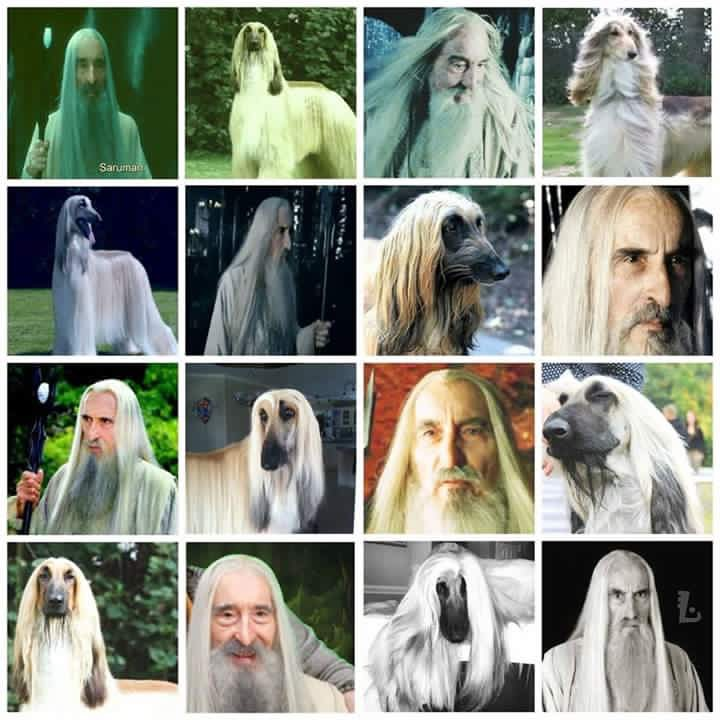
\includegraphics[height=2.3in]{img/dog-or-sarumon}};
        \end{tikzpicture}
    \end{center}

%\begin{center}
%\includegraphics[width=0.985\textwidth]{img-presentation/dilbert}
%\end{center}
\end{frame}

\tikzstyle{yes}=[draw, rectangle, fill=green!30,minimum width=3cm, minimum height=0.8cm]
\tikzstyle{no}=[draw, rectangle, fill=yellow!30,minimum width=3cm, minimum height=0.8cm]
\tikzstyle{maybe}=[draw, rectangle, fill=yellow!30,minimum width=3cm, minimum height=0.8cm]

\begin{frame}
\frametitle<1-2>{Classify the Image}
\frametitle<3-4>{Classify the Image}
\frametitle<5->{Classify the Image}
\centering
\resizebox{\textwidth}{!}{
\begin{tikzpicture}
%\tikzstyle{yes}=[draw, rectangle, fill=green!30,minimum width=1in]
%\tikzstyle{no}=[draw, rectangle, fill=yellow!30,minimum width=1in]
%\tikzstyle{maybe}=[draw, rectangle, fill=yellow!30,minimum width=1in]

\uncover<1>{
\node (image) at (0,0.25) {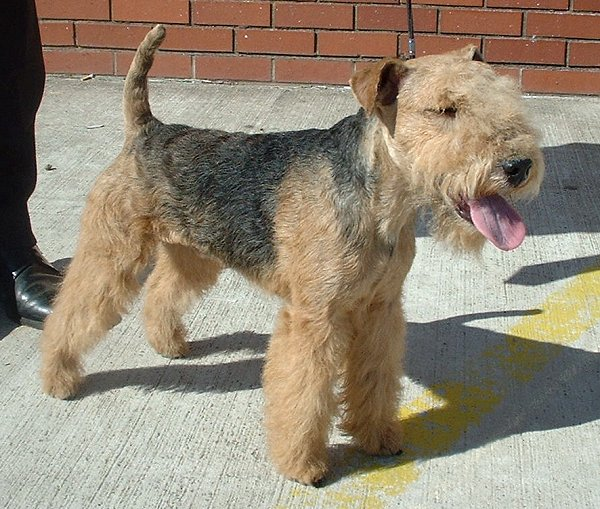
\includegraphics[height=2.25in]{img/Lakeland_Terrier}};
\node[maybe] at (-2,-4) {Animal};
\node[maybe] at (2,-4) {Not-Animal};
}

\uncover<2>{
\node (image) at (0,0.25) {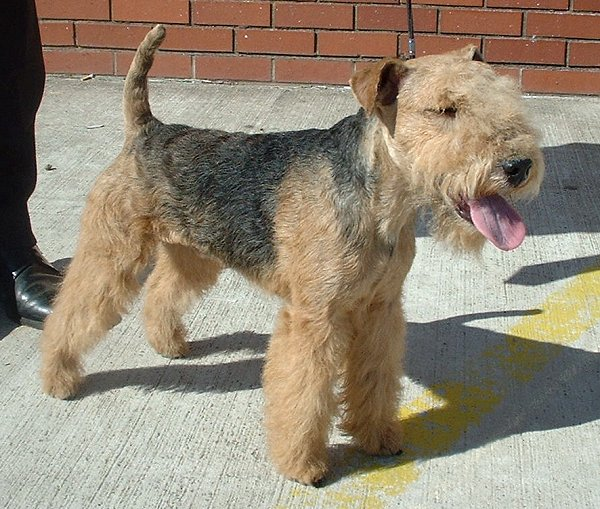
\includegraphics[height=2.25in]{img/Lakeland_Terrier}};
\node[yes] at (-2,-4) {Animal};
\node[maybe] at (2,-4) {Not-Animal};
}

\uncover<3>{
\node (image) at (0,0.25) {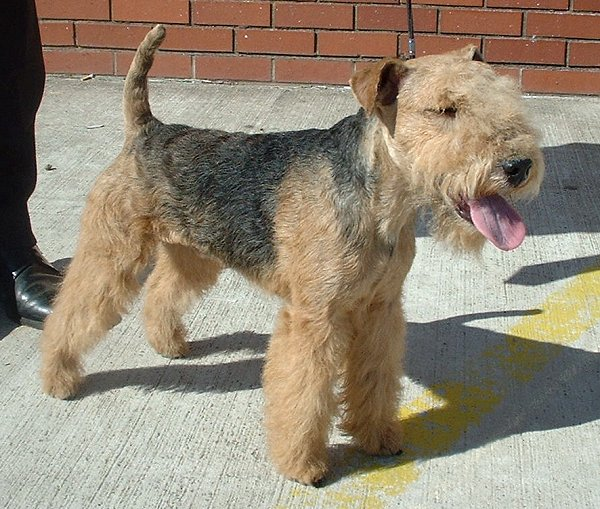
\includegraphics[height=2.25in]{img/Lakeland_Terrier}};
\node at (-3.25,-3) {\footnotesize Animal};
\node at (3.5,-3) {\footnotesize Not-Animal};
\draw (-6.5,-3.325) -- (-0.25, -3.325);
\draw (6.5,-3.325) -- (0.25, -3.325);
\node[maybe] at (-5,-4) {Fish};
\node[maybe] at (-1.6875,-4) {Bird};
\node[maybe] at (1.6875,-4) {Vehicle};
\node[maybe] at (5,-4) {Plant};
\node[maybe] at (-5,-5) {Insect};
\node[maybe] at (-1.6875,-5) {Mammal};
\node[maybe] at (1.6875,-5) {Building};
\node[maybe] at (5,-5) {Object};
}

\uncover<4>{
\node (image) at (0,0.25) {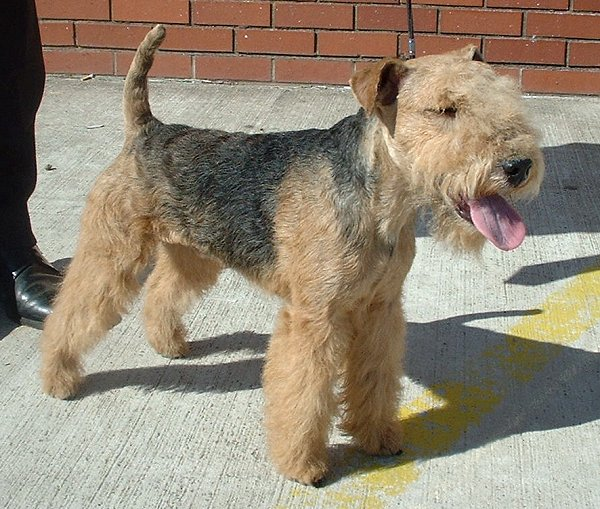
\includegraphics[height=2.25in]{img/Lakeland_Terrier}};
\node at (-3.25,-3) {\footnotesize Animal};
\node at (3.5,-3) {\footnotesize Not-Animal};
\draw (-6.5,-3.325) -- (-0.25, -3.325);
\draw (6.5,-3.325) -- (0.25, -3.325);
\node[maybe] at (-5,-4) {Fish};
\node[maybe] at (-1.6875,-4) {Bird};
\node[maybe] at (1.6875,-4) {Vehicle};
\node[maybe] at (5,-4) {Plant};
\node[maybe] at (-5,-5) {Insect};
\node[yes] at (-1.6875,-5) {Mammal};
\node[maybe] at (1.6875,-5) {Building};
\node[maybe] at (5,-5) {Object};
}

%\uncover<4>{
%\node (image) at (0,0.25) {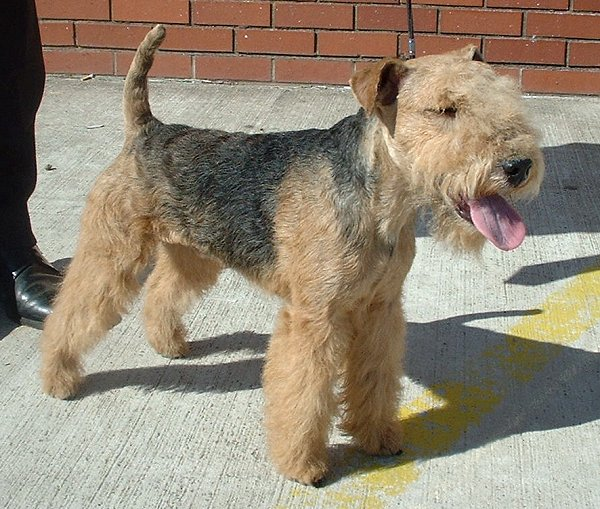
\includegraphics[height=2.25in]{img/Lakeland_Terrier}};
%\node at (-3.25,-3) {\footnotesize Animal};
%\node at (3.5,-3) {\footnotesize Not-Animal};
%\draw (-6.5,-3.325) -- (-0.25, -3.325);
%\draw (6.5,-3.325) -- (0.25, -3.325);
%\node[maybe] at (-5,-4) {Cat};
%\node[yes] at (-1.6875,-4) {Dog};
%\node[maybe] at (1.6875,-4) {Car};
%\node[maybe] at (5,-4) {Tree};
%\node[maybe] at (-5,-5) {Horse};
%\node[maybe] at (-1.6875,-5) {Fish};
%\node[maybe] at (1.6875,-5) {House};
%\node[maybe] at (5,-5) {Hat};
%}

\uncover<5>{
\node (image) at (0,0.25) {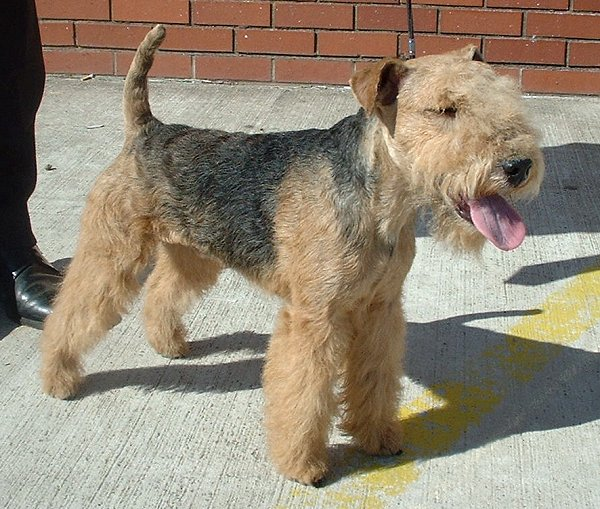
\includegraphics[height=2.25in]{img/Lakeland_Terrier}};
\node at (0,-3.5) {\Large ImageNet has 1000 different classes};
\node at (0,-4.5) {\Large (80 different dog breeds)};
    %\node at (0,-5) {\Large generalization error = $O(\sqrt{k/n})$};
}

\uncover<6>{
\node (image) at (0,0.25) {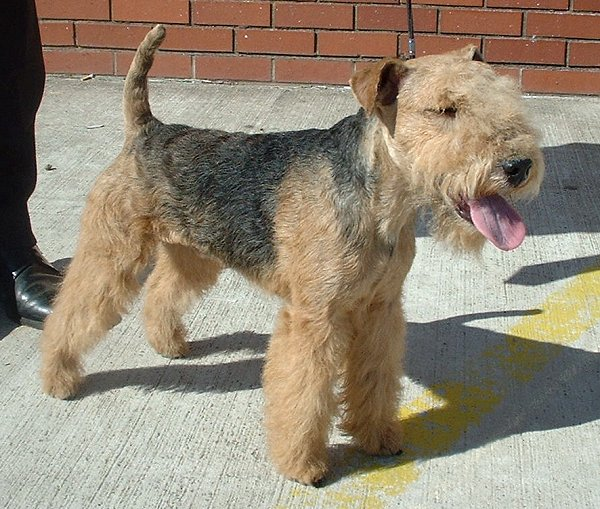
\includegraphics[height=2.25in]{img/Lakeland_Terrier}};
\node[maybe] at (-5,-4) {Irish Terrier};
\node[maybe] at (-1.6875,-4) {Airedale};
%\node[maybe] at (1.6875,-4) {Horse};
%\node[maybe] at (5,-4) {Human};
\node[maybe] at (-5,-5) {Lakeland Terrier};
\node[maybe] at (-1.6875,-5) {Irish Spaniel};
%\node[maybe] at (1.6875,-5) {House};
%\node[maybe] at (5,-5) {Hat};
\node at (3.5,-4.5) {Note shown: 996 other classes};
}

\uncover<7>{
\node (image) at (0,0.25) {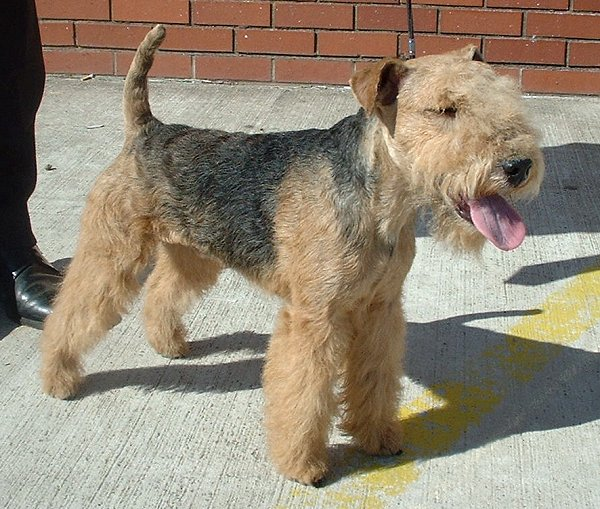
\includegraphics[height=2.25in]{img/Lakeland_Terrier}};
\node[maybe] at (-5,-4) {Irish Terrier};
\node[maybe] at (-1.6875,-4) {Airedale};
\node[yes] at (-5,-5) {Lakeland Terrier};
\node[maybe] at (-1.6875,-5) {Irish Spaniel};
\node at (3.5,-4.5) {Note shown: 996 other classes};
}

\uncover<8>{
\node (image) at (0,0.25) {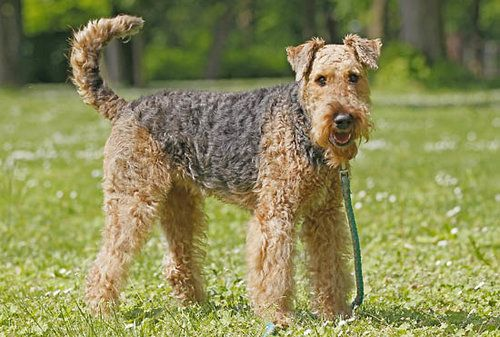
\includegraphics[height=2.25in]{img/Airedale}};
\node[maybe] at (-5,-4) {Irish Terrier};
\node[yes] at (-1.6875,-4) {Airedale};
\node[maybe] at (-5,-5) {Lakeland Terrier};
\node[maybe] at (-1.6875,-5) {Irish Spaniel};
\node at (3.5,-4.5) {Note shown: 996 other classes};
}

\uncover<9>{
\node (image) at (0,0.25) {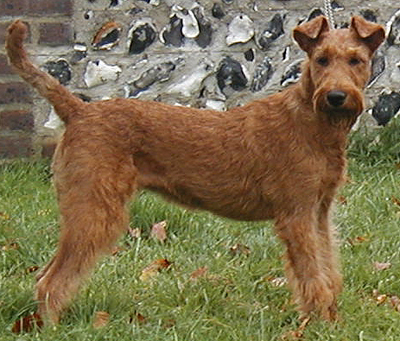
\includegraphics[height=2.25in]{img/Irish-Terrier}};
\node[yes] at (-5,-4) {Irish Terrier};
\node[maybe] at (-1.6875,-4) {Airedale};
\node[maybe] at (-5,-5) {Lakeland Terrier};
\node[maybe] at (-1.6875,-5) {Irish Spaniel};
\node at (3.5,-4.5) {Note shown: 996 other classes};
}

\uncover<10>{
\node (image) at (0,0.25) {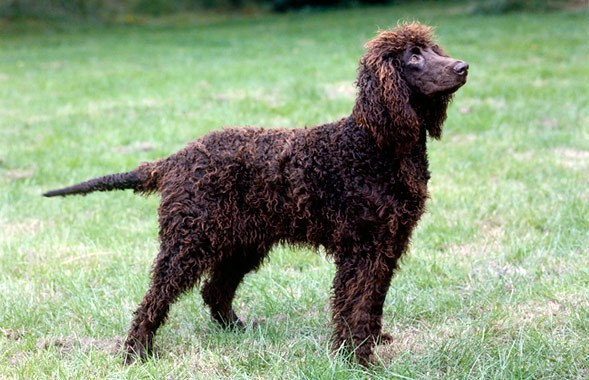
\includegraphics[height=2.25in]{img/water_spaniel}};
\node[maybe] at (-5,-4) {Irish Terrier};
\node[maybe] at (-1.6875,-4) {Airedale};
\node[maybe] at (-5,-5) {Lakeland Terrier};
\node[yes] at (-1.6875,-5) {Irish Spaniel};
\node at (3.5,-4.5) {Note shown: 996 other classes};
}

%\uncover<11> {
    %\node at (0, 2) {\Large more classes $\Rightarrow$ harder problem};
%
    %\node at (0, 0) {\Large real world problems are highly structured };
%
    %\node at (0, -2) {\Large \textbf{This talk:} exploit class structure to make the problem easier};
%}

\end{tikzpicture}
}
\end{frame}

%%%%%%%%%%%%%%%%%%%%%%%%%%%%%%%%%%%%%%%%%%%%%%%%%%%%%%%%%%%%%%%%%%%%%%%%%%%%%%%%

\ignore{
\begin{frame}
\frametitle{(Informal) Main Idea}

%ImageNet: 1000 classes, 80 breeds of dogs

Classification gets ``harder'' when we
\begin{itemize}
\item add more classes
\item the classes are ``more similar''
\end{itemize}

\vspace{0.2in}
This talk:
\begin{itemize}
\item formalize ``harder'' (machine learning)
\item formalize ``more similar'' (discrete geometry)
\item fix the problem
\end{itemize}

\end{frame}
}

\ignore{
\begin{frame}
\frametitle{ImageNet}

\begin{center}
%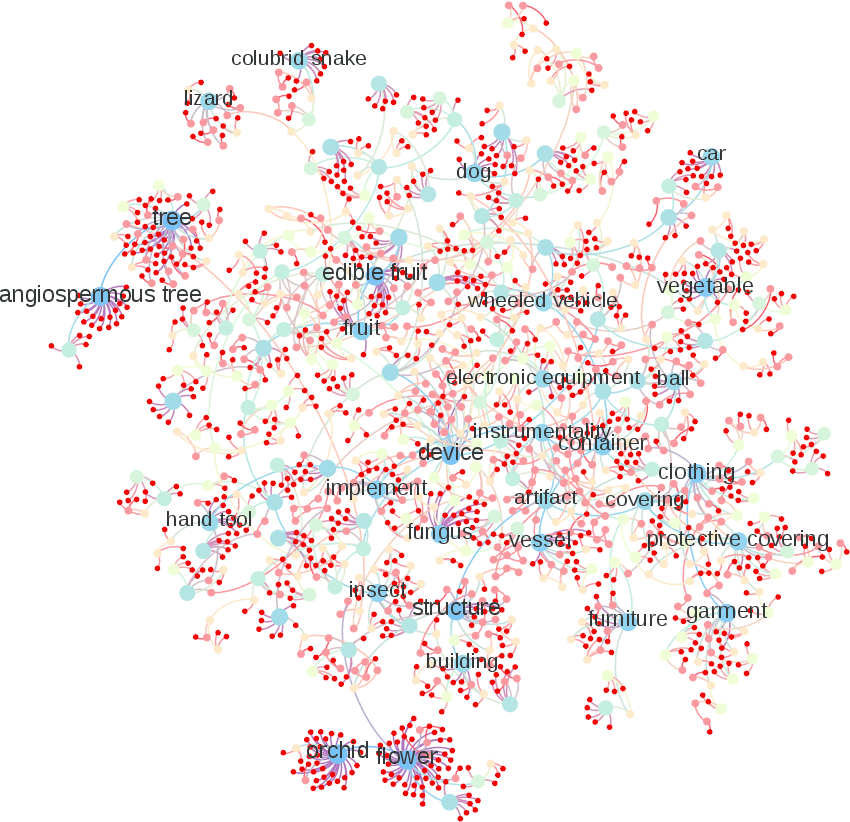
\includegraphics[height=2.7in]{img/imagenet-hierarchy}
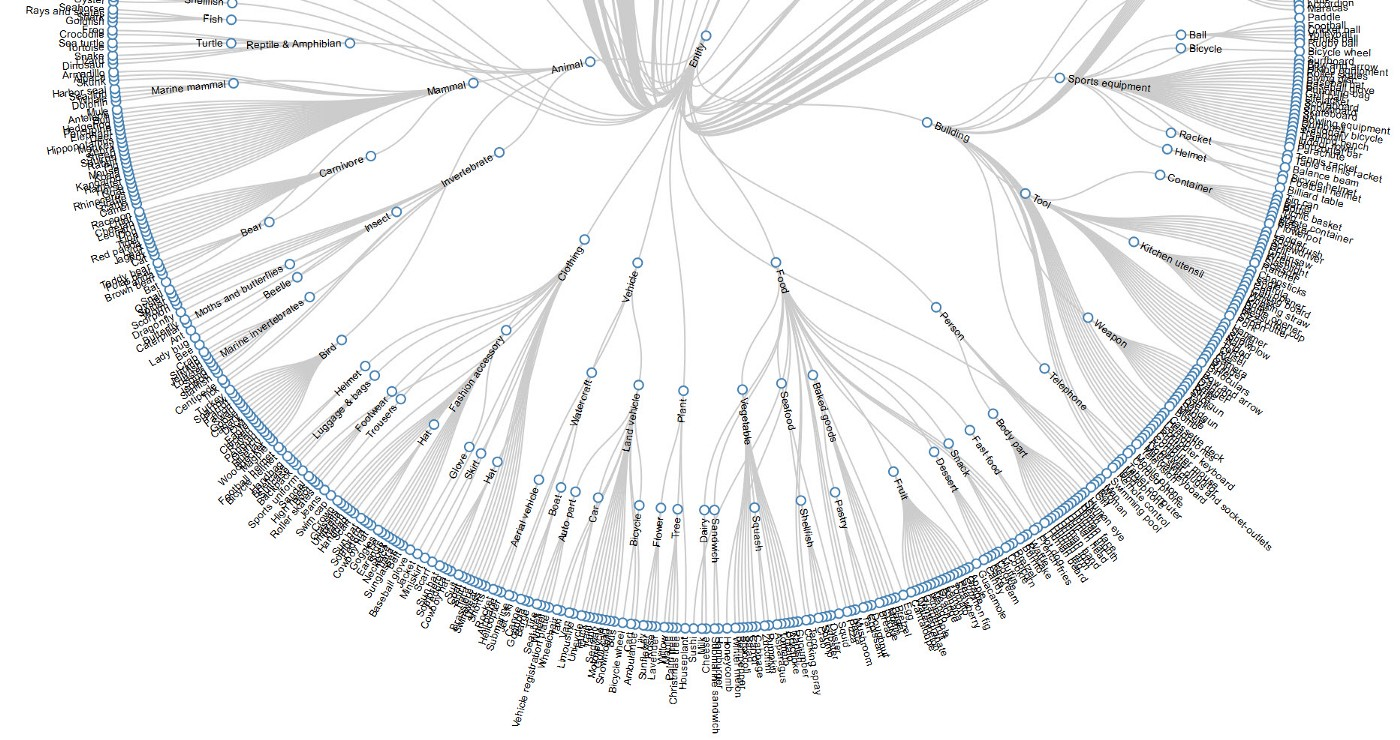
\includegraphics[width=\textwidth]{img/dendrogram}
\end{center}

1000 classes, hierarchically structured, 80 breeds of dog

{\tiny Image source: \citet{akata2014contributions}}
\end{frame}

%%%%%%%%%%%%%%%%%%%%%%%%%%%%%%%%%%%%%%%%

\begin{frame}
\frametitle{ImageNet}

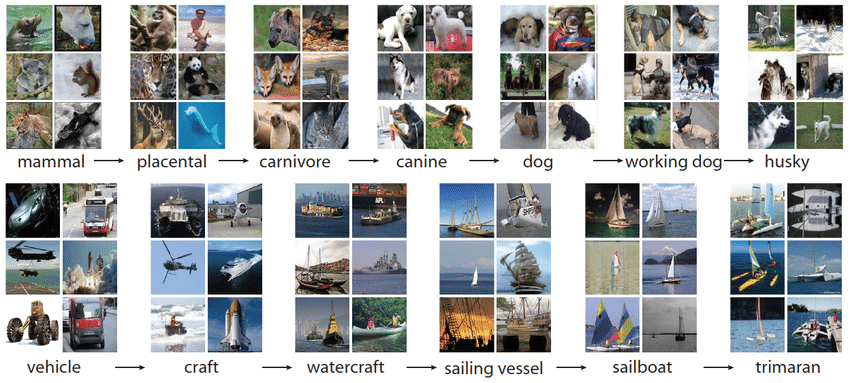
\includegraphics[width=\textwidth]{img/dog-trimaran}

{\tiny Image source: \citet{deng2012large}}
\end{frame}
}

%%%%%%%%%%%%%%%%%%%%%%%%%%%%%%%%%%%%%%%%

\begin{frame}
\frametitle{Real world data has lots of structure}

%ImageNet
%\begin{itemize}
%\item Most important image dataset
%\item 1.2 million images
%\item 1000 classes
%\item hierarchically structured
%\item 80 breeds of dog
%\end{itemize}
ImageNet has 1000 classes, hierarchical (DAG) class structure:

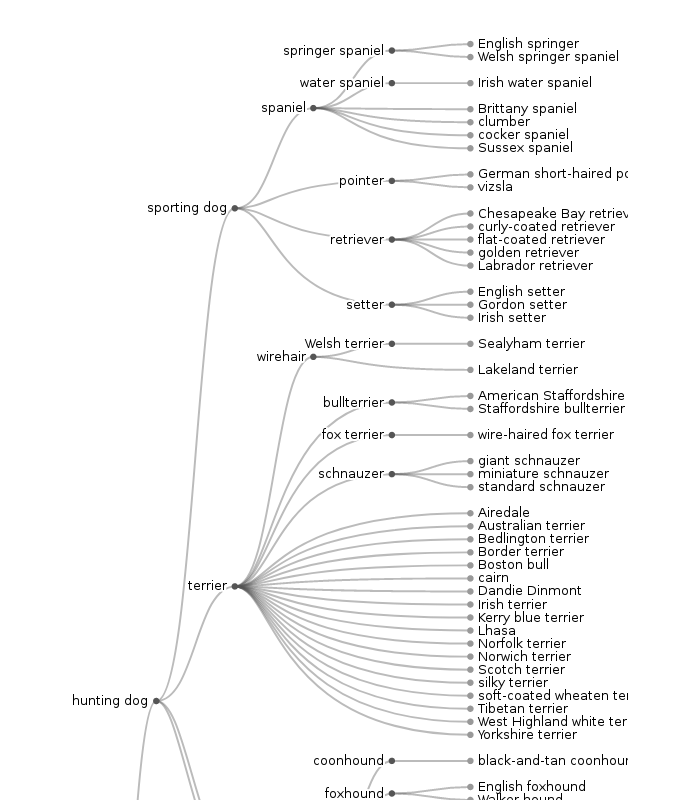
\includegraphics[height=2in]{img/imagent-hierarchy}

\vspace{0.25in}
Browse the hierarchy
\begin{itemize}
\item
\url{https://observablehq.com/@mbostock/imagenet-hierarchy}
\end{itemize}

\end{frame}

%%%%%%%%%%%%%%%%%%%%%%%%%%%%%%%%%%%%%%%%

\begin{frame}
\frametitle{Visualize this structure many ways}

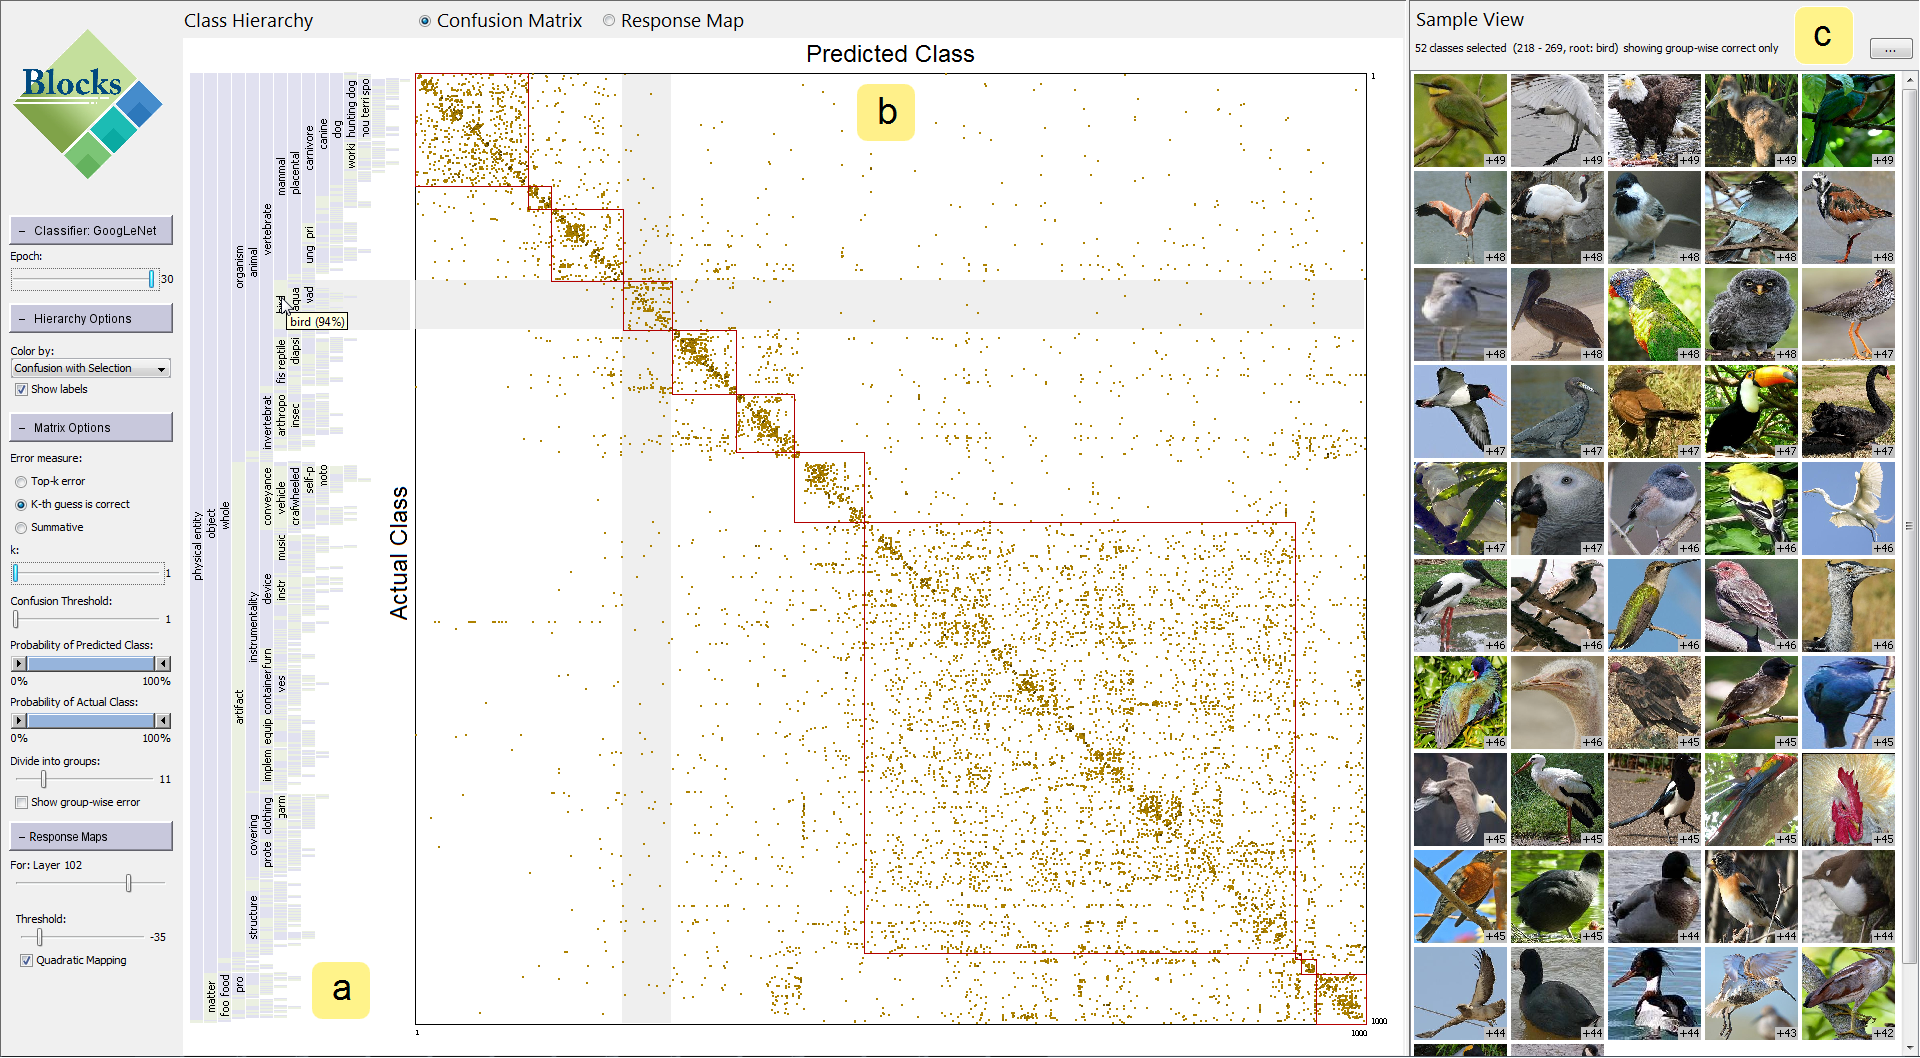
\includegraphics[width=\textwidth]{img/teaser}

{\tiny Image source: \citet{bilal2018}}
\end{frame}


\begin{frame}{Summary (so far)}

\begin{itemize}
\item more classes $\Rightarrow$ harder problem
\begin{itemize}
\item $k$: num classes, $d$: num dimensions, $n$: num data points
\end{itemize}
\begin{equation*}
\text{(cross entropy) generalization error}
=
O\left(\sqrt{\frac{kd}{n}}\right)
~~~~~~~~~~
\end{equation*}
\item real world classes are highly structured

\begin{itemize}
\item the doubling dimension $c <\!\!< k$

\end{itemize}
\begin{equation*}
\text{(conjectured optimal) generalization error}
=
O\left(\sqrt{\frac{cd}{n}}\right)
~~~~~~~~~~~~~~~~~~~~~~~~~~~~~~.
\end{equation*}

\item \textbf{contribution:} $U$/$V$-tree loss exploits arbitrary metric structure

\begin{equation*}
\text{(tree loss) generalization error} = 
\begin{cases}
\sqrt{\frac{d\log k}{n}} & c\le 1 \\
\sqrt{\frac{dk^{1-1/c}}{n}} & c>1 \\
\end{cases}
\end{equation*}

\item \textbf{bonus:} best performance on synthetic and real world experiments

\end{itemize}

\vspace{-4in}
\begin{tikzpicture}
    \node at (0,0) {};
    \node at (0,4in) {};

    \node[anchor=north west,fill=white,minimum width=4.5in,minimum height=0.7in] at (0,2.94in) {};
    \node[anchor=north west,fill=white,minimum width=4.5in,minimum height=0.74in] at (0,2.04in) {};
    \node[anchor=north west,fill=white,minimum width=4.5in,minimum height=0.7in] at (0,1.04in) {};
    \node[anchor=north west,fill=white,minimum width=4.5in,minimum height=0.3in] at (0,0.3in) {};
\end{tikzpicture}
\end{frame}


\begin{frame}
\frametitle{Machine Learning Review}

\resizebox{!}{0.8\paperheight}{
\begin{tikzpicture}
    [ node distance = 0.15in
    ]
    \Large

\node
    [ inner sep=0
    ] (img) 
    {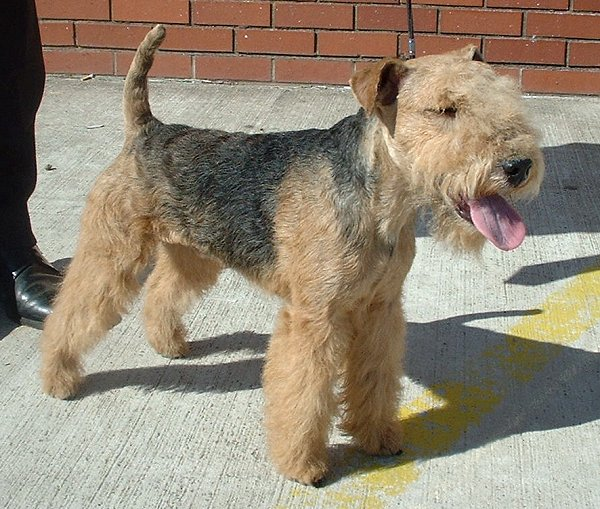
\includegraphics[width=3in]{img/Lakeland_Terrier}};

\uncover<1-3>{
\node
    [ below = of img
    , anchor=north
    , fill=darkgray
    , minimum height=1.15in
    , minimum width=3in
    , align=center
    , text centered
    , inner sep=0
    ]
    { \color{white} Machine Learning Model };
}

\uncover<4->{
\node 
    [ below = of img
    , anchor=north
    , fill=darkgray
    , minimum width=3in
    , minimum height=0.5in
    , align=center
    , inner sep=0
    , outer sep=0
    ](features)
    {\color{white}\centering Feature Generation};

\node
    [ below = of features
    , draw
    , text width = 3in
    , minimum height= 0.5in
    , align=center
    , inner sep=0
    , outer sep=0
    ](xentropy)
    {\parbox{\textwidth}{\centering Logistic Regression}};
\draw[->,line width=2pt] (features) -- (xentropy);
}

\uncover<1->{
\node
    [ below = 0.2in of xentropy
    , inner sep=0.1in
    , text width=2.8in
    , draw
    ]
    (classes)
    {
        %Class Predictions:
        %\vspace{0.1in}
        \begin{tikzpicture}
        %\small
        \tt
        \foreach  \l/\x[count=\y] in 
            { not-animal/4
            , animal/96
            }
        {\node[left,text width=1.0in] at (0,0.8*\y) {\l~~};
        \draw[draw=blue,fill={rgb,255:red,170; green,170; blue,255}] (0.0,0.8*\y-.3) rectangle (0.0+\x/100.0*3,0.8*\y+.3);
        \node[right] at (0.0+\x/100.0*3,.8*\y) {\x\!\%};
        }
        \end{tikzpicture}
    };
}

\draw[->,line width=2pt] (img) -- (features) ;
\draw[->,line width=2pt] (xentropy) -- (classes);

%%%%%%%%%%%%%%%%%%%%


\uncover<5,6>{
\node
    [right = 0.25in of features
    , text width = 5in
    ]
    (deep_place) {};

\node
    [ above = -2.0in of deep_place
    , text width = 5in
    ] (deep) {
    \baselineskip=16pt
    Highly domain specific\\
    ~\\
    \emph{Deep Learning} is state-of-the-art for images/text \\
    ~\\
    Lots of famous \emph{network architectures}:\\
    ~~~~LeNet \citep{lecun1998gradient} \\
    ~~~~AlexNet \citep{krizhevsky2012imagenet} \\
    ~~~~VGG \citep{simonyan2014very} \\
    ~~~~Inception v1 \citep{szegedy2015going} \\
    ~~~~Inception v2 \citep{ioffe2015batch} \\
    ~~~~Inception v3 \citep{szegedy2016rethinking} \\
    ~~~~Inception v4 \citep{he2016identity} \\
    ~~~~ResNet \citep{witten2016data} \\
    ~~~~ResNet2 \citep{he2016identity} \\
    %~~~~WideResNet \citep{zagoruyko2016wide} \\
    %~~~~SqueezeNet \citep{iandola2016squeezenet} \\
    ~~~~MobileNet \citep{howard2017mobilenets} \\
    ~~~~DenseNet \citep{huang2017densely} \\
    ~~~~ResNext \citep{lin2018focal} \\
    ~~~~NASNet \citep{zoph2018learning} \\
    ~~~~PNASNet \citep{liu2018progressive} \\
    %~~~~SqueezeExcitationNet \citep{hu2018squeeze} \\
    %~~~~MobileNet2 \citep{sandler2018mobilenetv2} \\
    ~~~~... \emph{and many more} ... \\
    ~\\
    \textbf{No theoretical guarantees}
    };
    \draw [decorate,decoration={brace,mirror,amplitude=10pt,raise=4pt, aspect=0.6},yshift=0pt]
        (deep.north west) -- (deep.south west) node [black,midway,anchor = west,xshift=0.8cm] {};
    }

%\uncover<6>{\node at (3.5in,-3.25in) [ text width = 5in,align=center ] {\textbf{better than Humans in practice} };}
%\uncover<6>{\node at (3.5in,-3.5in) [ text width = 4in,align=center ] {\textbf{treat as black box} };}
%
%\uncover<7->{
%\node
    %[ right = 0.25in of features
    %, text width = 3in
    %] (rd) {
        %Outputs a vector $\R^d$, $d$ is the number of features
    %};
    %}

\uncover<8->{
\node
    [ right = 0.25in of xentropy
    , text width = 6in
    ] (deep) {
        \baselineskip=16pt
        ~\\
        Known since the 1800s, good theoretical properties\\
        \vspace{0.15in}
        Let $d$ be number of features,\\
        \hspace{0.33in}$k$ be number of classes,\\
        \hspace{0.33in}$n$ be number of data points,\\
        then the generalization error = $\Theta\left(\sqrt{\frac{kd}{n}}\right)$
        \\
        \vspace{0.15in}
        \textbf{So more classes requires more data}
        ~\\
        %Known since at least \citet{nelder1972generalized}
    };
    \draw [decorate,decoration={brace,mirror,amplitude=10pt,raise=4pt},yshift=0pt]
        (deep.north west) -- (deep.south west) node [black,midway,anchor = west,xshift=0.8cm] {};
};
\end{tikzpicture}
}
\end{frame}

\begin{frame}
\frametitle{Machine Learning Review: What is Generalization Error?}

Standard Experimental Design:
\begin{itemize}
\item Split data into training/test set
\item Train model on training set
\item Evaluate model on the test set
\end{itemize}

%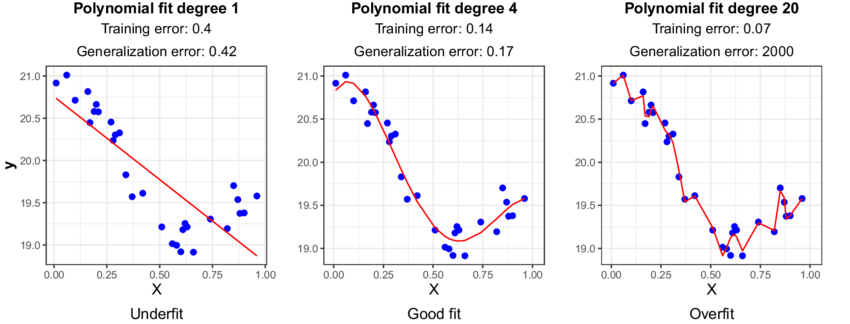
\includegraphics[width=\textwidth]{img/llustration-of-the-underfitting-overfitting-issue-on-a-simple-regression-case-Data}

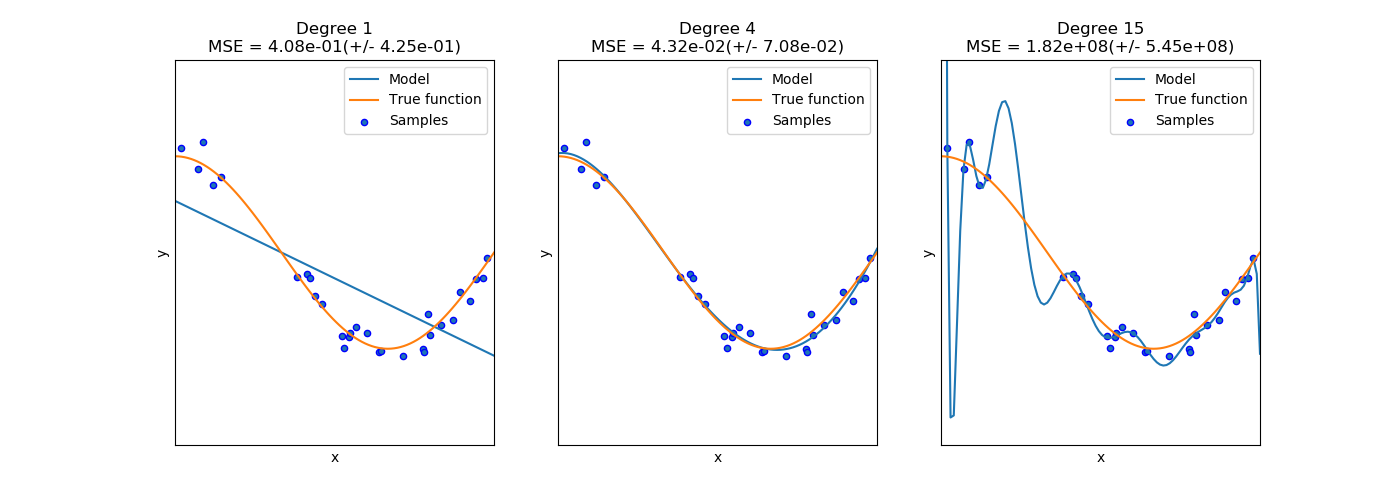
\includegraphics[width=\textwidth]{img/over-under-fit}

{
\fontsize{4}{4}
{\tiny Image source:} \url{https://scikit-learn.org/stable/auto_examples/model_selection/plot_underfitting_overfitting.html}
}
\end{frame}


\begin{frame}{Summary (so far)}

\begin{itemize}
\item more classes $\Rightarrow$ harder problem
\begin{itemize}
\item $k$: num classes, $d$: num dimensions, $n$: num data points
\end{itemize}
\begin{equation*}
\text{(cross entropy) generalization error}
=
O\left(\sqrt{\frac{kd}{n}}\right)
~~~~~~~~~~
\end{equation*}
\item real world classes are highly structured

\begin{itemize}
\item the doubling dimension $c <\!\!< k$

\end{itemize}
\begin{equation*}
\text{(conjectured optimal) generalization error}
=
O\left(\sqrt{\frac{cd}{n}}\right)
~~~~~~~~~~~~~~~~~~~~~~~~~~~~~~.
\end{equation*}

\item \textbf{contribution:} $U$/$V$-tree loss exploits arbitrary metric structure

\begin{equation*}
\text{(tree loss) generalization error} = 
\begin{cases}
\sqrt{\frac{d\log k}{n}} & c\le 1 \\
\sqrt{\frac{dk^{1-1/c}}{n}} & c>1 \\
\end{cases}
\end{equation*}

\item \textbf{bonus:} best performance on synthetic and real world experiments

\end{itemize}

\vspace{-4in}
\begin{tikzpicture}
    \node at (0,0) {};
    \node at (0,4in) {};

    %\node[anchor=north west,fill=white,minimum width=4.5in,minimum height=0.7in] at (0,2.94in) {};
    \node[anchor=north west,fill=white,minimum width=4.5in,minimum height=0.74in] at (0,2.04in) {};
    \node[anchor=north west,fill=white,minimum width=4.5in,minimum height=0.7in] at (0,1.04in) {};
    \node[anchor=north west,fill=white,minimum width=4.5in,minimum height=0.3in] at (0,0.3in) {};
\end{tikzpicture}
\end{frame}


\newtheorem{defn}{Definition}
\begin{frame}[fragile]{Metric spaces generalize euclidean space}
\centering
\resizebox{!}{4.5cm}{
\begin{tikzpicture}[dot/.style={circle,inner sep=2pt,fill,name=#1},
    extended line/.style={shorten >=-#1,shorten <=-#1},
    extended line/.default=1cm]

% draw the grid
\uncover<1-3> {
    \draw[->] (0,-0.25) -- (0,5.25) ;
    \draw[->] (-0.25,0) -- (5.25,0) ;
    \foreach \i in {1,...,5} {
        \draw[dotted] (-0.25,\i) -- (5.25,\i);
        \draw[dotted] (\i,-0.25) -- (\i,5.25);
    }
}

% draw the points
\uncover<1-3> {
    \node [dot=a,label=above left:a] at (1,1) {};
    \node [dot=b,label=above:b] at (2,4) {};
    \node [dot=c,label=above right:c] at (4,2) {};
}

% draw the L2 metric
\uncover<1> {
    \draw (a) -- (b) -- (c) -- (a);
    \node at (3,1.25) {$\sqrt{10}$};
    \node at (1,2.75) {$\sqrt{10}$};
    \node at (3.5,3.25) {$2\sqrt{2}$};
    \node at (8, 4.5) {
        Euclidean distance:
        };
    \node at (9,2.5) {

        $\begin{aligned}
        \mathcal{X}& = \mathbb{R}^p \\
        \displaystyle
        d(x,y)
        &=
        \displaystyle
        \left(\sum_{i=1}^p (x_i-y_i)^2\right)^{\frac 1 2} \\
        \end{aligned}$
        };
    \node at (9, 0.5) { Runtime to calculate distance: $O(p)$ };
}

% draw the L1 metric
\uncover<2> {
    \draw (a) -- (1,4) -- (b) -- (4,4) -- (c) -- (4,1) -- (a);
    \node at (2.5,1.25) {$4$};
    \node at (1.25,2.75) {$4$};
    \node at (3.5,3.5) {$4$};
    \node at (9, 4.5) {
        $L_1$ (Manhattan, taxicab) distance:
        };
    \node at (9,2.5) {
        $\begin{aligned}
        \mathcal{X}& = \mathbb{R}^p \\
        \displaystyle
        d(x,y)
        &=
        \displaystyle
        \sum_{i=1}^p |x_i-y_i| \\
        \end{aligned}$
        };
    \node at (9, 0.5) { Runtime to calculate distance: $O(p)$ };
}

% draw the Linf metric
\uncover<3> {
    \draw (a) -- (1,4);
    \draw (4,4) -- (c);
    \draw (a) -- (4,1);
    \node at (2.5,1.25) {$3$};
    \node at (1.25,2.75) {$3$};
    \node at (3.5,3.5) {$2$};
    \node at (8, 4.5) {
        $L_\infty$ (sup) distance:
        };
    \node at (9,2.5) {
        $\begin{aligned}
        \mathcal{X}& = \mathbb{R}^p \\
        \displaystyle
        d(x,y)
        &=
        \displaystyle
        \sup_{i\in\{1..p\}} |x_i-y_i| \\
        \end{aligned}$
        };
    \node at (9, 0.5) { Runtime to calculate distance: $O(p)$ };
}

%% draw the Lebesgue metric
%\uncover<4> {
    %\node at (9, 4.5) {
        %Lebesgue family of distances:
        %};
    %\node at (9,2.5) {
        %$\begin{aligned}
        %\mathcal{X}& = \mathbb{R}^n \\
        %\displaystyle
        %d(x,y)
        %&=
        %\displaystyle
        %\left(\sum_{i\in\{1..n\}} |x_i-y_i|^n\right)^{\frac 1 n} \\
        %\end{aligned}$
        %};
    %\node at (9, 0.5) { Runtime to calculate distance: $O(n)$ };
%}

%% graph distances
%\uncover <6-7> {
    %\draw[color=red,line width=2pt] (3.35,3.1) -- (3.65,3.4);
    %\node[color=red] at (4,3.25) {\textbf{1?}};
%}
%\uncover<6> {
    %\draw[color=red,line width=2pt] (6,0) -- (12,5);
%}

%\uncover<5-6> {
    %\draw (a) -- (b) -- (c) -- (a);
    %\node at (3,1.25) {$2$};
    %\node at (1,2.75) {$4$};
    %\node at (3.5,3.25) {$5$};
    %\node at (9, 4.5) {
        %weighted, fully-connected graph distance
        %};
    %\node at (9,2.5) {
        %$\begin{aligned}
        %\mathcal{X}& = \{a,b,c\} \\
        %\displaystyle
        %d(x,y)
        %&=
        %\text{edge weight}
        %\end{aligned}$
        %};
    %\node at (9, 0.5) { Runtime to calculate distance: $O(1)$ };
%}

%% graph distances
%\uncover<7> {
    %\draw (a) -- (b) -- (c) -- (a);
    %\node at (3,1.25) {$2$};
    %\node at (1,2.75) {$4$};
    %\node at (3.5,3.25) {$5$};
    %\node at (9, 4.5) {
        %Dijkstra graph distance
        %};
    %\node at (9,2.5) {
        %$\begin{aligned}
        %\mathcal{X}& = \{a,b,c\} \\
        %\displaystyle
        %d(x,y)
        %&=
        %\text{shortest path between $x$ and $y$}
        %\end{aligned}$
        %};
    %\node at (9, 0.5) { Runtime to calculate distance: $O(e+v\log v)$ };
%}

%% graph distances
%\uncover<8> {
    %\draw (a) -- (b);
    %\draw (c) -- (a);
    %\node at (3,1.25) {$2$};
    %\node at (1,2.75) {$4$};
    %\node at (9, 4.5) {
        %Dijkstra graph distance
        %};
    %\node at (9,2.5) {
        %$\begin{aligned}
        %\mathcal{X}& = \{a,b,c\} \\
        %\displaystyle
        %d(x,y)
        %&=
        %\text{shortest path between $x$ and $y$}
        %\end{aligned}$
        %};
    %\node at (9, 0.5) { Runtime to calculate distance: $O(e+v\log v)$ };
%}

%% graph distances
%\uncover<9> {
    %\draw (a) -- (b);
    %\node at (1,2.75) {$4$};
    %\node at (9, 4.5) {
        %Dijkstra graph distance
        %};
    %\node at (9,2.5) {
        %$\begin{aligned}
        %\mathcal{X}& = \{a,b,c\} \\
        %\displaystyle
        %d(x,y)
        %&=
        %\text{shortest path between $x$ and $y$}
        %\end{aligned}$
        %};
    %\node at (9, 0.5) { Runtime to calculate distance: $O(e+v\log v)$ };
%}

%% graph distances
%\uncover<10> {
    %\node at (8, 4.5) {
        %trivial distance
        %};
    %\node at (9,2.5) {
        %$\begin{aligned}
        %\mathcal{X}& = \{a,b,c\} \\
        %\displaystyle
        %d(x,y)
        %&=
        %\infty
        %\end{aligned}$
        %};
    %\node at (9, 0.5) { Runtime to calculate distance: $O(1)$ };
%}

%% graph distances
%\uncover<11> {
    %\node at (1,3) {
        %$d \left(
        %\text{
        %\begin{tikzpicture}
        %\node at (0,2) {};
        %\node [dot= ] at (1,1) {};
        %\node [dot= ] at (1,0) {};
        %\node [dot= ] at (0,1) {};
        %\draw (1,1) -- (1,0) -- (0,1) -- (1,1);
        %\end{tikzpicture}
        %,
        %\begin{tikzpicture}
        %\node at (0,2) {};
        %\node [dot= ] at (1,1) {};
        %\node [dot= ] at (1,0) {};
        %\node [dot= ] at (0,1) {};
        %\node [dot= ] at (0,0) {};
        %\draw (1,1) -- (1,0) -- (0,1) -- (1,1) -- (0,0) -- (0,1) -- (1,0) -- (0,0);
        %\end{tikzpicture}
        %}
        %\right)$
    %};
    %\node at (9, 4.5) {
        %\emph{graph metrics} are distances between graphs
        %};
    %\node at (9,2.5) {
        %$\begin{aligned}
        %\mathcal{X}& = \text{set of all graphs} \\
        %\displaystyle
        %d(x,y)
        %&=
        %\text{many possibilities}
        %\end{aligned}$
        %};
    %\node at (9, 0.5) { Runtime to calculate distance: $O(1)$ };
%}

\end{tikzpicture}
}
\begin{defn}
A \emph{metric space} is a set $\mathcal{X}$ equiped with a distance function $d : \mathcal{X} \times \mathcal{X} \rightarrow \mathbb{R}$ such that:
\begin{center}
\begin{tabular}{ll}
$d(x,y) \ge 0$ & $d(x,y) = 0$ iff $x=y$ \\
$d(x,y) = d(y,x)$ & $d(x,z) \le d(x,y) + d(y,z)$ \\
\end{tabular}
\end{center}
\end{defn}
\end{frame}



\newcommand\mybox[2][]{\tikz[overlay]\node[fill=lightyellow,inner sep=2pt, anchor=text, rectangle, rounded corners=1mm,draw=black,#1] {#2};\phantom{#2}}

\tikzstyle{reddot}=[draw=black,line width=1pt,minimum size=1.5mm,inner sep=0pt,outer sep=0pt,shape=circle,fill=blue]
\tikzstyle{bluedot}=[draw=blue,minimum size=0.5mm,inner sep=0pt,outer sep=0pt,shape=circle,fill=blue]

%%%%%%%%%%%%%%%%%%%%%%%%%%%%%%%%%%%%%%%%%%%%%%%%%%%%%%%%%%%%%%%%%%%%%%%%%%%%%%%%
\begin{frame}{How structured is a metric space?}

%Many ways to measure (equilateral, Minkowski-Bouligand, Hausdorff, ...)
That is, what is it's dimension?

\pause
\vspace{0.1in}
We'll use the \emph{doubling dimension} $c$
 
\pause
\vspace{0.1in}
Captures the idea of an ``intrinsic'' dimension of a space

\pause
\begin{center}
\begin{tikzpicture}[scale=0.67]
% draw the grid
\draw[->] (0,-0.25) -- (0,5.25) ;
\draw[->] (-0.25,0) -- (5.25,0) ;
\foreach \i in {1,...,5} {
    \draw[dotted,draw=gray] (-0.25,\i) -- (5.25,\i);
}
\foreach \i in {1,...,5} {
    \draw[dotted,draw=gray] (\i,-0.25) -- (\i,5.25);
}

\draw[loosely dotted,draw=blue,line width=2pt] (1,2) to[in=225,out=-45] (4.5,2);
\path[loosely dotted,draw=blue,line width=2pt] (1.5,3.5) circle (0.5);
\draw[loosely dotted,draw=blue,line width=2pt] (3.5,3.5) to (4.5,3.5);

\node[anchor=north west] at (1.75,-0.2) {$c \approx 1$};

\end{tikzpicture}
\hspace{0.5in}
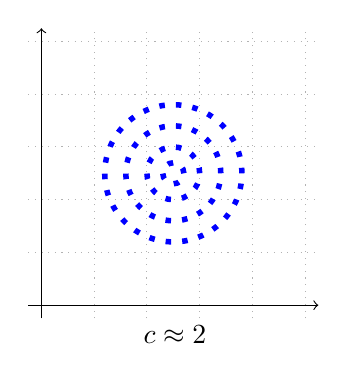
\begin{tikzpicture}[scale=0.67]
% draw the grid
\draw[->] (0,-0.25) -- (0,5.25) ;
\draw[->] (-0.25,0) -- (5.25,0) ;
\foreach \i in {1,...,5} {
    \draw[dotted,draw=gray] (-0.25,\i) -- (5.25,\i);
}
\foreach \i in {1,...,5} {
    \draw[dotted,draw=gray] (\i,-0.25) -- (\i,5.25);
}

%\draw[loosely dotted,draw=blue,line width=2pt] (1,2) to[in=225,out=-45] (4.5,2);
\path[loosely dotted,draw=blue,line width=2pt] (2.5,2.5) circle (0.2);
\path[loosely dotted,draw=blue,line width=2pt] (2.5,2.5) circle (0.5);
\path[loosely dotted,draw=blue,line width=2pt] (2.5,2.5) circle (0.9);
\path[loosely dotted,draw=blue,line width=2pt] (2.5,2.5) circle (1.3);
%\draw[loosely dotted,draw=blue,line width=2pt] (3.5,3.5) to (4.5,3.5);

\node[anchor=north west] at (1.75,-0.2) {$c \approx 2$};

\end{tikzpicture}
\end{center}

%\textbf{Theorem:} In any Euclidean space $\R^d$, the doubling dimension = $O(d)$

\pause
\vspace{0.1in}
    \textbf{
$c$ small $\Rightarrow$ lots of structure; $c$ large $\Rightarrow$ little structure
}

\end{frame}

%%%%%%%%%%%%%%%%%%%%%%%%%%%%%%%%%%%%%%%%%%%%%%%%%%%%%%%%%%%%%%%%%%%%%%%%%%%%%%%%

\begin{frame}{The doubling dimension $c$}

A set $C$ is a \textbf{$\delta$-covering} of $X$ if for all $x\in X$, there exists a $c \in C$ such that $\dist{x}{c} \le \delta$.
The \textbf{covering number} of $X$, denoted $N_\delta(X)$, is the cardinality of the smallest $\delta$-covering.
The \textbf{doubling constant} is 
\begin{equation}
2^c = \max_{x\in X,\delta>0} N_\delta( B(x,2\delta))
.
\end{equation}

%
%An \textbf{$r$-covering} of a set $X$ is a subset of $X$ such that all pairwise distances are greater than $r$. %$\{x_1,x_2,...x_M\} \subset X$ such that $\dist{x_i}{x_j} > r$ for all distinct $i,j$.
%
%The \textbf{$r$-packing number} $M_r (X)$ is the cardinality of the largest $r$-packing.
%

\vspace{0.1in}
\hrule
\vspace{0.1in}
%%%%%%%%%%%%%%%%%%%%%%%%%%%%%%%%%%%%%%%%

\begin{tikzpicture}[scale=0.67]
% draw the grid
\draw[->] (0,-0.25) -- (0,5.25) ;
\draw[->] (-0.25,0) -- (5.25,0) ;
\foreach \i in {1,...,5} {
    \draw[dotted,draw=gray] (-0.25,\i) -- (5.25,\i);
}
\foreach \i in {1,...,5} {
    \draw[dotted,draw=gray] (\i,-0.25) -- (\i,5.25);
}

%\foreach \i in {1,...,10} {
    %\foreach \j in {1,...,10} {
        %\node[bluedot] at (0.3*\i,0.3*\j) {};
    %}
%}
\node[bluedot] at (2.5,2.5) {};
\foreach \i in {1,...,10} {
    \node[bluedot] at (2.5+0.2*\i,2.5-0.2*\i) {};
    \node[bluedot] at (2.5-0.2*\i,2.5+0.2*\i) {};
}

\uncover<2-5> {
\node[reddot]  at (2.5,2.5) {};
\path[draw=black] (2.5,2.5) circle (1.4);
\path[draw=black] (2.5,2.5) circle (2.85);

\node[reddot]  at (1.3,3.7) {};
\path[draw=black] (1.3,3.7) circle (1.4);
\node[reddot]  at (3.7,1.3) {};
\path[draw=black] (3.7,1.3) circle (1.4);
}

\uncover<2-5> {
%\node[fill=white] at (1.5,0) {\textcolor{darkgreen}{robust}};
%\node at (2.5,-1) {\textcolor{darkgreen}{$c=O(d)$}} ;
}
\end{tikzpicture}
%%%%%%%%%%%%%%%%%%%%
\begin{tikzpicture}[scale=0.67]
% draw the grid
\draw[->] (0,-0.25) -- (0,5.25) ;
\draw[->] (-0.25,0) -- (5.25,0) ;
\foreach \i in {1,...,5} {
    \draw[dotted,draw=gray] (-0.25,\i) -- (5.25,\i);
}
\foreach \i in {1,...,5} {
    \draw[dotted,draw=gray] (\i,-0.25) -- (\i,5.25);
}

\node[bluedot] at (2.5,2.5) {};
\foreach \i in {1,...,6} {
    \node[bluedot] at (3.3+0.2*\i,1.7-0.2*\i) {};
    \node[bluedot] at (1.7-0.2*\i,3.3+0.2*\i) {};
}

\uncover<3-5>{
\node[reddot] at (2.5,2.5) {};
\path[draw=black] (2.5,2.5) circle (1.4);
\path[draw=black] (2.5,2.5) circle (2.85);

\node[reddot]  at (1.3,3.7) {};
\path[draw=black] (1.3,3.7) circle (1.4);
\node[reddot]  at (3.7,1.3) {};
\path[draw=black] (3.7,1.3) circle (1.4);
}
\uncover<3-5> {
%\node[fill=white] at (1.5,0) {\textcolor{darkgreen}{robust}};
%\node at (2.5,-1) {\textcolor{darkgreen}{$c=O(d)$}} ;
}
\end{tikzpicture}
%%%%%%%%%%%%%%%%%%%%
\begin{tikzpicture}[scale=0.67]
% draw the grid
\draw[->] (0,-0.25) -- (0,5.25) ;
\draw[->] (-0.25,0) -- (5.25,0) ;
\foreach \i in {1,...,5} {
    \draw[dotted,draw=gray] (-0.25,\i) -- (5.25,\i);
}
\foreach \i in {1,...,5} {
    \draw[dotted,draw=gray] (\i,-0.25) -- (\i,5.25);
}

\node[bluedot] at (2.5,2.5) {};
\path[loosely dotted,draw=blue,line width=0.5mm] (2.5,2.5) circle (1.73);

\uncover<4-5>{
\node[reddot] at (2.5,2.5) {};
\path[draw=black] (2.5,2.5) circle (1.4);
\path[draw=black] (2.5,2.5) circle (2.85);
}
\uncover<4-5>   {
\node[reddot]  at (1.3,3.7) {};
\path[draw=black] (1.3,3.7) circle (1.4);
\node[reddot]  at (3.7,3.7) {};
\path[draw=black] (3.7,3.7) circle (1.4);
\node[reddot]  at (3.7,1.3) {};
\path[draw=black] (3.7,1.3) circle (1.4);
\node[reddot]  at (1.3,1.3) {};
\path[draw=black] (1.3,1.3) circle (1.4);

    %\node[fill=white] at (1.5,0) {\textcolor{darkgreen}{robust}};
    %\node at (2.5,-1) {\textcolor{darkgreen}{$c=O(d)$}};
}
\end{tikzpicture}

%\uncover<5>{
%\vspace{-2.80in}
%\begin{tikzpicture}
%\node[fill=lightyellow,draw=black,thick,text width=11.05cm,rounded corners=0.1cm,inner sep=0.2in] at (0,0) { 
    %\textcolor{darkgreen}{Advantage: robust to all changes in the data set}
    %\\
    %\textcolor{red}{Disadvantage: cannot be used for exact nearest neighbor queries}
%};
%\end{tikzpicture}
%}
%
%\vspace{1.8in}

\end{frame}


\begin{frame}
\frametitle{Optimal Generalization Error}

\textbf{Recall:} standard generalization error bound is $\Theta(\sqrt{kd/n})$

\pause
\begin{block}{Conjecture}
If the classes have metric structure with doubling dimension $c$,
then 
\begin{equation}
\text{the optimal generalization error} = \Theta\left(\sqrt{cd/n}\right)
\end{equation}
\end{block}

\pause
Why?
\pause
\begin{itemize}
    \item if the metric is discrete (no assumptions), then $c=\Theta(k)$ recovering known bound
    \pause
\item if the metric is $\mathbb Z$, $k=\infty, c=\Theta(1)$ and the known bound is $O(\sqrt{d/n})$ via Poisson regression
    \pause
\item if the metric is $m$-sphere, then $c=\Theta(m)$ and prior work shows the bound is $O(\sqrt{md/n})$
via MvMF regression \citep{izbicki2019exploiting}
\end{itemize}

\end{frame}


\begin{frame}{Summary (so far)}

\begin{itemize}
\item more classes $\Rightarrow$ harder problem
\begin{itemize}
\item $k$: num classes, $d$: num dimensions, $n$: num data points
\end{itemize}
\begin{equation*}
\text{(cross entropy) generalization error}
=
O\left(\sqrt{\frac{kd}{n}}\right)
~~~~~~~~~~
\end{equation*}
\item real world classes are highly structured

\begin{itemize}
\item the doubling dimension $c <\!\!< k$

\end{itemize}
\begin{equation*}
\text{(conjectured optimal) generalization error}
=
O\left(\sqrt{\frac{cd}{n}}\right)
~~~~~~~~~~~~~~~~~~~~~~~~~~~~~~.
\end{equation*}

\item \textbf{contribution:} $U$/$V$-tree loss exploits arbitrary metric structure

\begin{equation*}
\text{(tree loss) generalization error} = 
\begin{cases}
\sqrt{\frac{d\log k}{n}} & c\le 1 \\
\sqrt{\frac{dk^{1-1/c}}{n}} & c>1 \\
\end{cases}
\end{equation*}

\item \textbf{bonus:} best performance on synthetic and real world experiments

\end{itemize}

\vspace{-4in}
\begin{tikzpicture}
    \node at (0,0) {};
    \node at (0,4in) {};

    %\node[anchor=north west,fill=white,minimum width=4.5in,minimum height=0.7in] at (0,2.94in) {};
    %\node[anchor=north west,fill=white,minimum width=4.5in,minimum height=0.74in] at (0,2.04in) {};
    \node[anchor=north west,fill=white,minimum width=4.5in,minimum height=0.7in] at (0,1.04in) {};
    \node[anchor=north west,fill=white,minimum width=4.5in,minimum height=0.3in] at (0,0.3in) {};
\end{tikzpicture}
\end{frame}



\begin{frame}{Multiclass Classification I: Loss Function}

\vspace{0.1in}
The standard cross entropy loss is defined to be
\begin{equation}
    \label{eq:xentropy}
    \ell(W;(\x,y)) = - \log \frac {\exp(-\trans\w_y \x)}{\sum_{j=1}^k \exp(-\trans \w_j \x)}
\vspace{-0.1in}
\end{equation}
where
\begin{itemize}
    %\item $(\x, y)$ is an input data point
    \item $\x \in \R^d$ is an input feature vector
    \item $y \in \{1, 2, ..., k\}$ is the input class label
    \item $\w_i \in \R^d$ is the parameter vector for class $i$
    \item $W = (\w_1, \w_2, ..., \w_k) \in \R^{d\times k}$ is the parameter matrix
\end{itemize}

\uncover<2>{
\vspace{0.2in}
    \textbf{Goal:} Approximate the optimal parameter matrix
\begin{equation}
    W^* = \argmin_{W} \E \ell(W; (\x,y))
    .
\end{equation}
}
\end{frame}

%%%%%%%%%%%%%%%%%%%%%%%%%%%%%%%%%%%%%%%%%%%%%%%%%%%%%%%%%%%%%%%%%%%%%%%%%%%%%%%%
\begin{frame}{Multiclass Classification II: SGD}

Approximate $W^*$ using \emph{stochastic gradient descent} (SGD):
\begin{equation}
    W_{t+1} = W_t - \eta \nabla \ell(W_t, (\x_t, y_t))
\end{equation}
where $\eta$ is the step size/learning rate.

%\vspace{0.2in}
%As $t \to \infty$, $W_t \to W^*$.

%\vspace{0.2in}
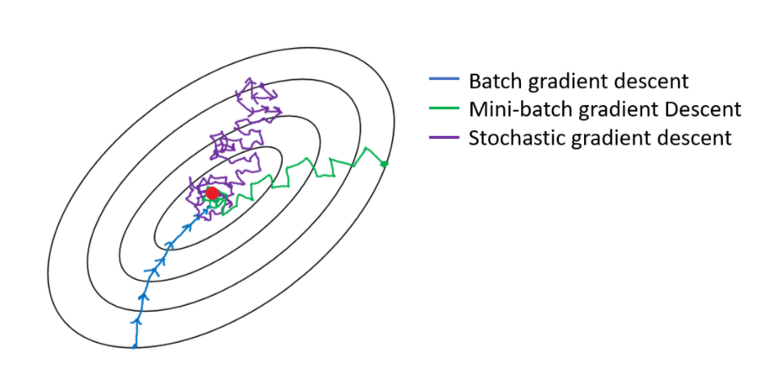
\includegraphics[height=2in]{img/sgd}

{\tiny
Image Source: \url{https://sweta-nit.medium.com/batch-mini-batch-and-stochastic-gradient-descent-e9bc4cacd461}
}
\end{frame}

%%%%%%%%%%%%%%%%%%%%%%%%%%%%%%%%%%%%%%%%%%%%%%%%%%%%%%%%%%%%%%%%%%%%%%%%%%%%%%%%
\ignore{
\begin{frame}{SGD}
We let $\theta^{(t)}$ denote the parameter value at iteration $t$,
and $\eta : \mathbb R$ be the step size.
Let $\nu_t$ be a noisy gradient of $f$ satisfying
\begin{equation}
    \E[\nu_t | \theta^{(t)}] = \nabla f(\theta^{(t)}).
\end{equation}
Then the parameter update for step $t$ is defined to be
\begin{equation}
    \theta^{(t+1)} = \theta^{(t)} - \eta \nabla \nu_t
    .
\end{equation}
When using parameter averaging, the final model parameters are defined to be
\begin{equation}
    \bar\theta = \frac1T \sum_{i=1}^T \theta^{(t)}
    .
\end{equation}
\end{frame}
}
%%%%%%%%%%%%%%%%%%%%%%%%%%%%%%%%%%%%%%%%%%%%%%%%%%%%%%%%%%%%%%%%%%%%%%%%%%%%%%%%
\ignore{
\begin{frame}{Multiclass Classification II: Objectives}

The \emph{true loss} is defined to be
\begin{equation}
    L_D(W) = \E_{(\x,y)\sim D} \ell(W; (\x, y))
\end{equation}
where $D$ is the unknown data distribution.

\vspace{0.2in}
The \emph{optimal parameter matrix} is 
\begin{equation}
    W^* = \argmin_{W} L_D(W)
\end{equation}

\end{frame}
}

\begin{frame}{Key Observation}

\begin{block}{Lemma 1 (informal)}
SGD satisfies
\begin{equation}
\text{generalization error} = O\left( \frac{\lF{\nabla \ell}}{\sqrt n} \right)
\end{equation}
\end{block}

\begin{itemize}
\item
Immediate corrollary of standard properties of SGD

\citep{shalev2014understanding}

\vspace{0.2in}
\uncover<2->{
\item
Painful notation to formalize this
}

        \uncover<4->{
\vspace{0.2in}
\item Recover known bounds:
\begin{equation*}
\lF{\nabla\ell} = \lF{W^*} = O(\sqrt{kd})
\quad\Rightarrow
\text{generalization error} = O(\sqrt{kd/n})
\end{equation*}
}

%(IMNSO: most important skill for new mathematician to learn

\uncover<5>{
%\vspace{0.2in}
\item \textbf{Idea:} 
Rewrite the cross entropy loss so that $\lF{\nabla\ell}$ is smaller
\begin{itemize}
\vspace{0.1in}
\item For people familiar with the notation, this change is ``trivial''
\end{itemize}
}
\end{itemize}

\uncover<3> {
    \begin{center}
    \vspace{-3.45in}
    \setlength{\fboxsep}{0pt}%
    \setlength{\fboxrule}{1pt}%
    \fbox{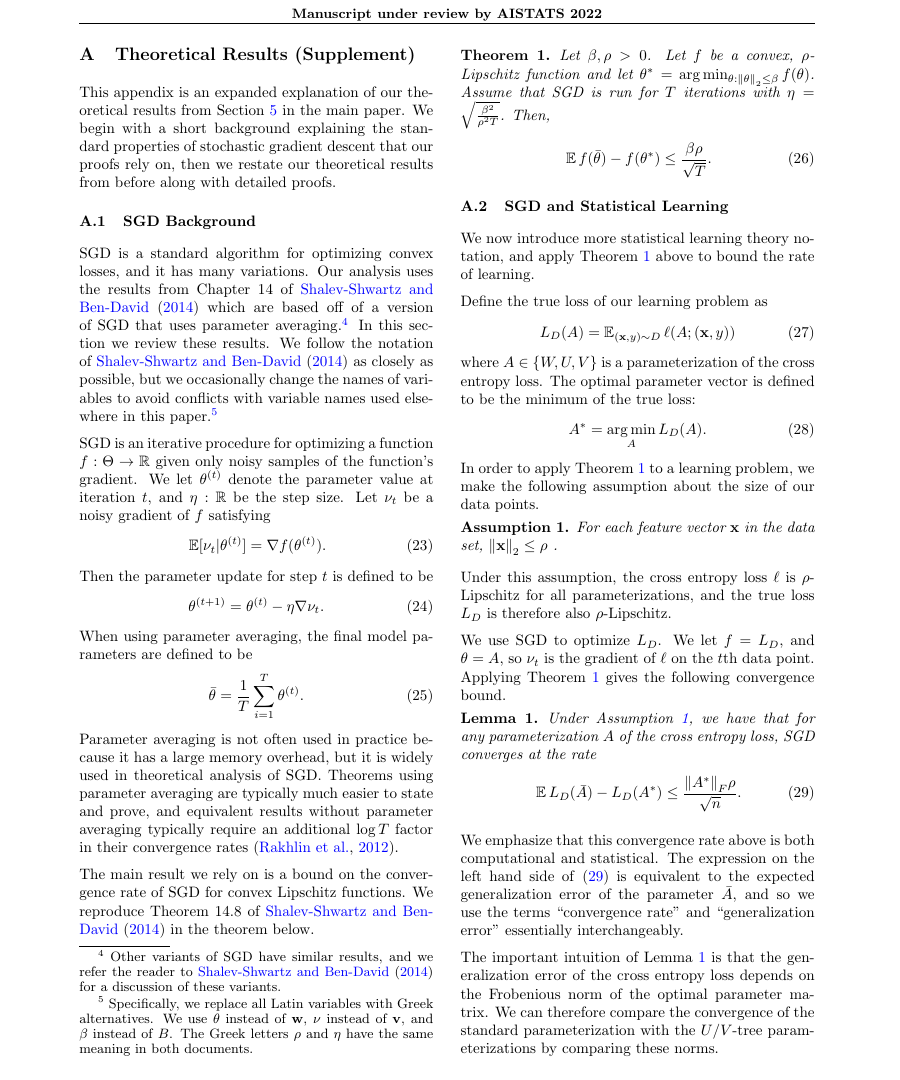
\includegraphics[height=3.5in]{img/lemma1-paper}}
    \end{center}
}
\uncover<5> {~}

\end{frame}

%%%%%%%%%%%%%%%%%%%%%%%%%%%%%%%%%%%%%%%%%%%%%%%%%%%%%%%%%%%%%%%%%%%%%%%%%%%%%%%%

%\begin{frame}{Key Ideas}
%\begin{block}{Lemma 1 (informal)}
%\begin{equation}
%\text{generalization error} \le \frac{\beta\rho}
%\end{equation}
%\end{block}
%\end{frame}



\begin{frame}
\frametitle{Rewriting the cross entropy loss}
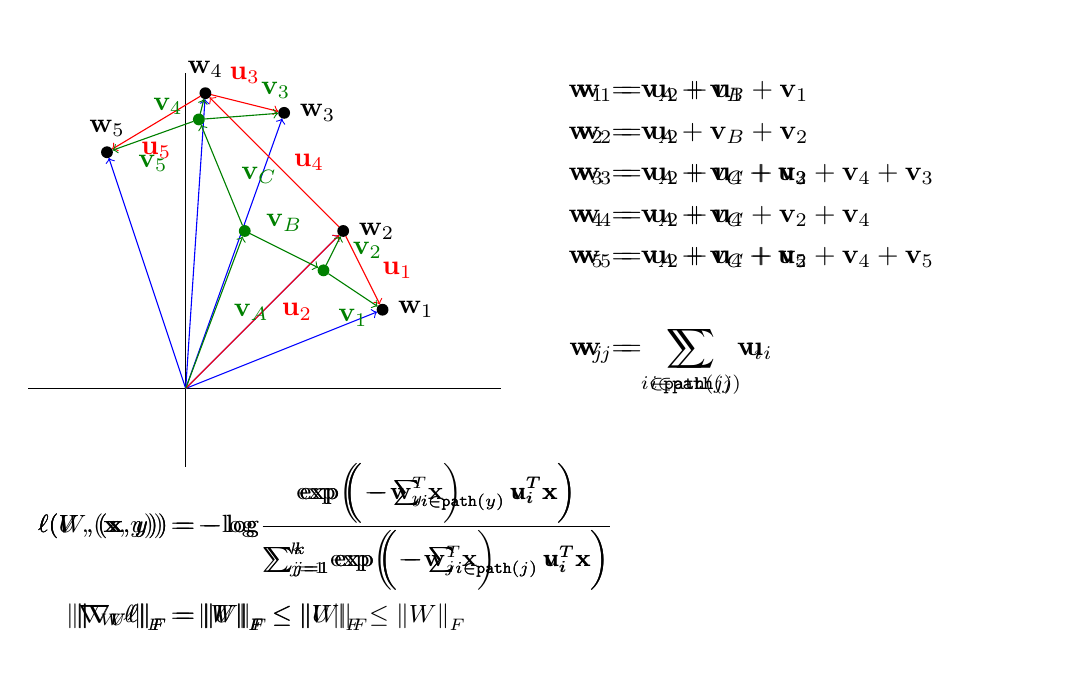
\begin{tikzpicture}
    [
    dot/.style = {minimum width=0.15cm,inner sep=0pt,line width=0pt,fill,circle,black,font=\small}
    ]
    \draw[] (0,4) -- (0,-1);
    \draw[] (4,0) -- (-2,0);
    \node[dot,label={0:$\w_1$}] (w1) at (2.5,1) {};
    \node[dot,label={0:$\w_2$}] (w2) at (2,2) {};
    \node[dot,label={90:$\w_4$}] (w4) at (0.25,3.75) {};
    \node[dot,label={0:$\w_3$}] (w3) at (1.25,3.5) {};
    \node[dot,label={$\w_5$}] (w5) at (-1,3) {};

    \uncover<1>{
    \draw[->,color=blue] (0,0) to (w1);
    \draw[->,color=blue] (0,0) to (w2);
    \draw[->,color=blue] (0,0) to (w3);
    \draw[->,color=blue] (0,0) to (w4);
    \draw[->,color=blue] (0,0) to (w5);

    \node[anchor=west] at (-2,-2.0) {
        \parbox{2in}{
        \small
        \begin{align*}
            \ell(W, (\x,y))
            &= 
    -\log \frac {\exp\bigg(-\trans\w_y \x\bigg)}{\sum_{j=1}^k \exp\bigg(-\trans \w_j \x\bigg)}
    \\
    \lF{\nabla_W\ell} &= \lF{W}
    \end{align*}
}};
    }

    \uncover<2>{
    \draw[->,color=red] (0,0) -- node[label={0:$\uu_2$}]{} (w2);
    \draw[->,color=red] (w2) -- node[label={0:$\uu_1$}]{} (w1);
    \draw[->,color=red] (w2) -- node[label={0:$\uu_4$}]{} (w4);
    \draw[->,color=red] (w4) -- node[label={$\uu_3$}]{} (w3);
    \draw[->,color=red] (w4) -- node[label={270:$\uu_5$}]{} (w5);

    \node[anchor=west] at (2.5,2) {
        \parbox{3in}{
        \begin{align*}
        \w_1 &= \uu_2 + \uu_1 \\
        \w_2 &= \uu_2 \\
        \w_3 &= \uu_2 + \uu_4 + \uu_3 \\
        \w_4 &= \uu_2 + \uu_4 \\
        \w_5 &= \uu_2 + \uu_4 + \uu_5 \\
        \\
        \w_j &= \sum_{i \in \ancestor(j)} \uu_i
        \end{align*}
    }
    };
    \node[anchor=west] at (-2,-2.0) {
        \parbox{2in}{
        \small
        \begin{align*}
            \ell(\rlap{$U$}\hphantom{W}, (\x,y))
            &= 
            -\log \frac {\exp\bigg(-\sum_{i\in\ancestor(y)}\trans\uu_i \x\bigg)}{\sum_{j=1}^k \exp\bigg(-\sum_{i\in\ancestor(j)}\trans\uu_i \x\bigg)}
    \\
        \lF{\nabla_U\ell} &= \lF{U} \le \lF{W}
    \end{align*}
    }};
    }

    \uncover<3>{
    \node[dot,color=darkgreen] (vC) at (0.1667,3.4167) {};
    \node[dot,color=darkgreen] (vB) at (1.75,1.5) {};
    \node[dot,color=darkgreen] (vA) at (0.75,2.0) {};

    \draw[->,color=darkgreen] (0,0) -- node[label={0:$\vv_A$}]{} (vA);
    \draw[->,color=darkgreen] (vA) -- node[label={90:$\vv_B$}]{} (vB);
    \draw[->,color=darkgreen] (vA) -- node[label={0:$\vv_C$}]{} (vC);
    \draw[->,color=darkgreen] (vB) -- node[label={270:$\vv_1$}]{} (w1);
    \draw[->,color=darkgreen] (vB) -- node[label={0:$\vv_2$}]{} (w2);
    \draw[->,color=darkgreen] (vC) -- node[label={40:$\vv_3$}]{} (w3);
    \draw[->,color=darkgreen] (vC) -- node[label={180:$\vv_4$}]{} (w4);
    \draw[->,color=darkgreen] (vC) -- node[label={270:$\vv_5$}]{} (w5);

    \node[anchor=west] at (3.25,2) {
    \parbox{3in}{
    \begin{align*}
    \w_1 &= \vv_A + \vv_B + \vv_1 \\
    \w_2 &= \vv_A + \vv_B + \vv_2 \\
    \w_3 &= \vv_A + \vv_C + \vv_2 + \vv_4 + \vv_3 \\
    \w_4 &= \vv_A + \vv_C + \vv_2 + \vv_4 \\
    \w_5 &= \vv_A + \vv_C + \vv_2 + \vv_4 + \vv_5 \\
    \\
    \w_j &= \sum_{i \in \ancestor(j)} \vv_i
    \end{align*}
}
};
    \node[anchor=west] at (-2,-2.0) {
        \parbox{2in}{
        \small
        \begin{align*}
            \ell(\rlap{$V$}\hphantom{W}, (\x,y))
            &= 
            -\log \frac {\exp\bigg(-\sum_{i\in\ancestor(y)}\trans\vv_i \x\bigg)}{\sum_{j=1}^k \exp\bigg(-\sum_{i\in\ancestor(j)}\trans\vv_i \x\bigg)}
    \\
        \lF{\nabla_V\ell} &= \lF{V} \le \lF{U} \le \lF{W}
    \end{align*}
    }};
}

\end{tikzpicture}

%\begin{align*}
%W &= (\w_1, \w_2, \w_3, \w_4, \w_5) \\
    %\color{red} U &= \color{red} (\uu_1, \uu_2, \uu_3, \uu_4, \uu_5) & \color{red} \lF{U} \le \lF{W} \\
%%V &= (\vv_A, \vv_B, \vv_C, \vv_1, \vv_2, \vv_3, \vv_4, \vv_5) & \lF{V} \le \lF{U} \le \lF{W} \\
%\end{align*}
    
\end{frame}
%%%%%%%%%%%%%%%%%%%%%%%%%%%%%%%%%%%%%%%%%%%%%%%%%%%%%%%%%%%%%%%%%%%%%%%%%%%%%%%%
\ignore{
\begin{frame}
\frametitle{U-tree}
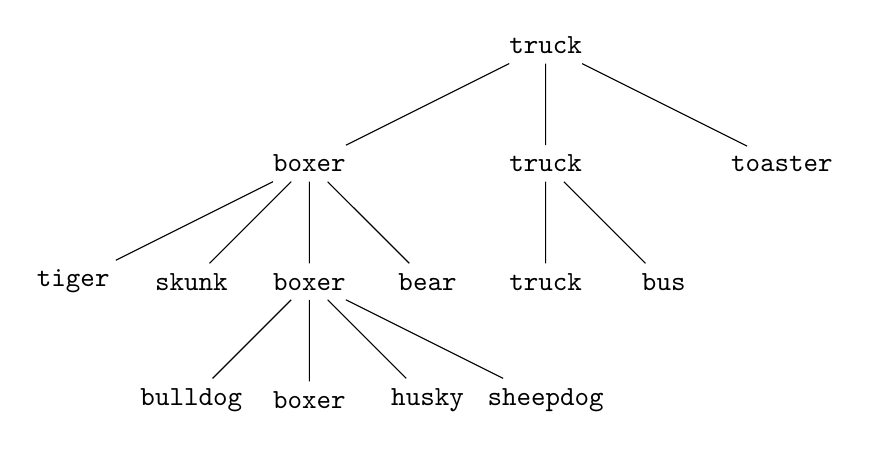
\begin{tikzpicture}
    [ level distance=1.5cm
    , level 1/.style={sibling distance=3cm}
    , level 2/.style={sibling distance=1.5cm}
    ]
\node {\texttt{truck}}
    child {node {\texttt{boxer}}
      child {node {\texttt{tiger}}}
      child {node {\texttt{skunk}}}
      child {node {\texttt{boxer}}
        child {edge from parent[draw=none]} % Added
        child {node {\texttt{bulldog}}}
        child {node {\texttt{boxer}}}
        child {node {\texttt{husky}}}
        child {node {\texttt{sheepdog}}}
      }
      child {node {\texttt{bear}}}
      child {edge from parent[draw=none]} % Added
      }
    child {node {\texttt{truck}}
      child {edge from parent[draw=none]} % Added
      child {node {\texttt{truck}}}
      child {node {\texttt{bus}}}
    }
    child {node {\texttt{toaster}}}
    ;

\end{tikzpicture}
\end{frame}
}

%%%%%%%%%%%%%%%%%%%%%%%%%%%%%%%%%%%%%%%%

\begin{frame}
\frametitle{Intuition}

$W$-parameterization learns everything from scratch

%Learning the Lakeland Terrier class from scratch is hard

\vspace{0.1in}
\begin{tabular}{m{0.7in}m{3.7in}}
    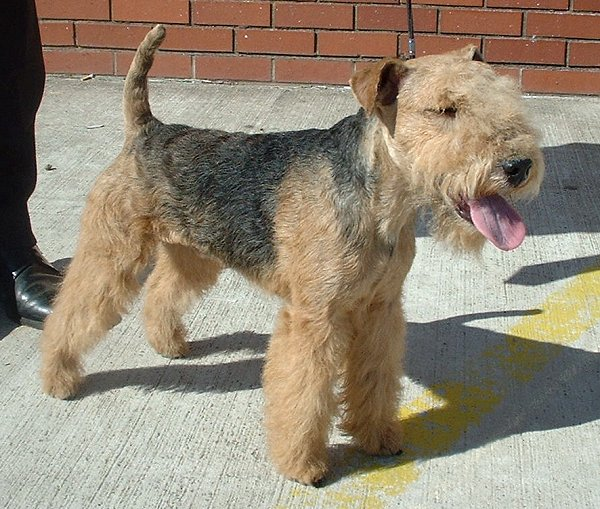
\includegraphics[height=0.5in]{img/Lakeland_Terrier} & How is \textbf{Lakeland Terrier} different than a tree? truck? person? horse? ... \\
    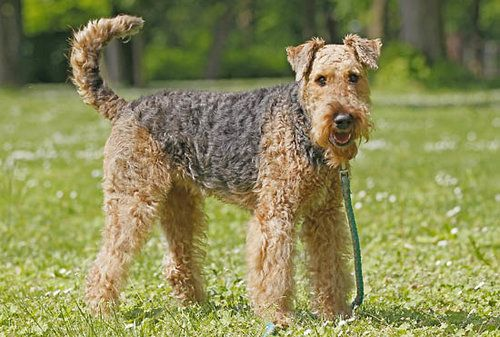
\includegraphics[height=0.5in]{img/Airedale} & How is \textbf{Airedale} different than a tree? truck? person? horse? ... \\
    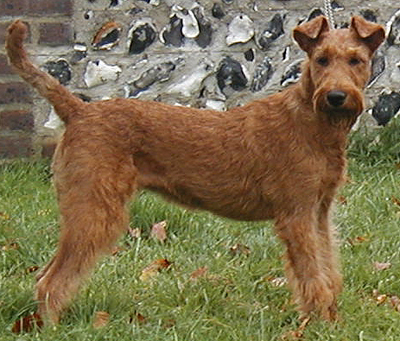
\includegraphics[height=0.5in]{img/Irish-Terrier} & How is \textbf{Irish Terrier} different than a tree? truck? person? horse? ... \\
    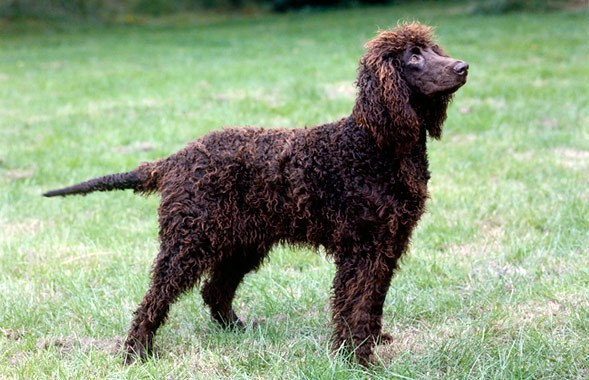
\includegraphics[height=0.5in]{img/water_spaniel} & How is \textbf{Irish Spaniel} different than a tree? truck? person? horse? ... \\
\end{tabular}
\end{frame}

\begin{frame}
\frametitle{Intuition}

$U$/$V$-tree parameterizations learn 1 class from scratch

\vspace{0.1in}
    \begin{tabular}{m{0.7in}m{3.8in}}
        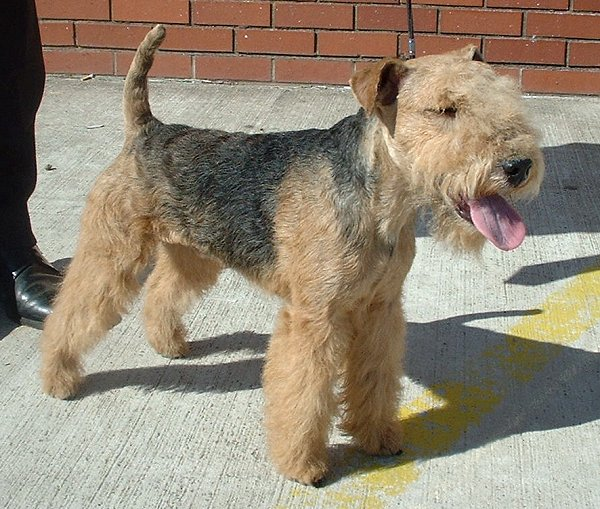
\includegraphics[height=0.5in]{img/Lakeland_Terrier} & How is \textbf{Lakeland Terrier} different than a tree? truck? person? horse? ... \\
\end{tabular}

\vspace{0.2in}
Learns only the difference between related classes

    \vspace{0.1in}
\begin{tabular}{m{0.7in}m{3.8in}}
    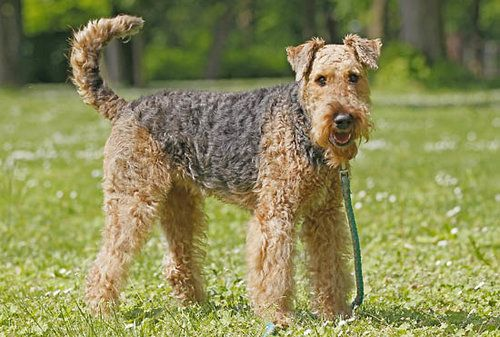
\includegraphics[height=0.5in]{img/Airedale} & \textbf{Airedale} is a big Lakeland Terrier \\
    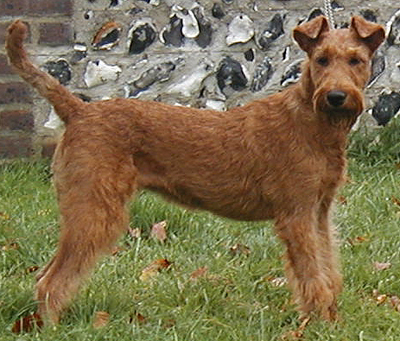
\includegraphics[height=0.5in]{img/Irish-Terrier} & \textbf{Irish Terrier} is a Lakeland Terrier with brown fur \\
    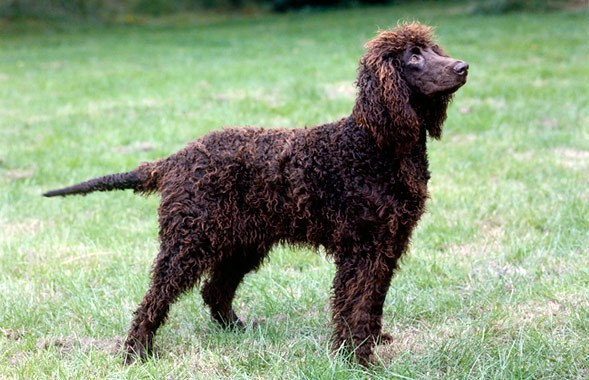
\includegraphics[height=0.5in]{img/water_spaniel} & \textbf{Irish Spaniel} is a Lakeland Terrier with long dark fur and big ears\\
\end{tabular}
\ignore{
\pause
    \vspace{0.3in}
Learn related classes by analogy (i.e.\ learn the difference)

    \vspace{0.1in}
\begin{tabular}{m{0.7in}m{3.8in}}
    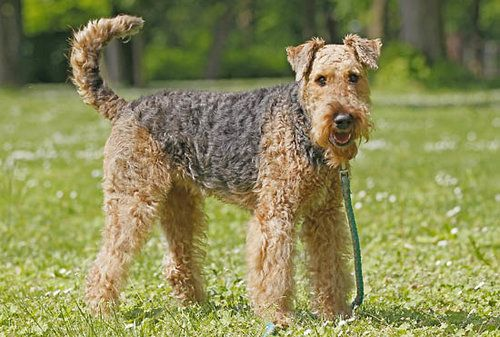
\includegraphics[height=0.5in]{img/Airedale} & Airedale is a big Lakeland Terrier \\
    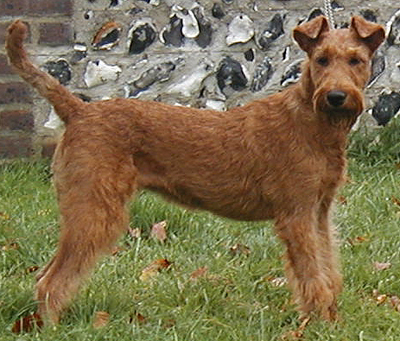
\includegraphics[height=0.5in]{img/Irish-Terrier} & Irish Terrier is a Lakeland Terrier with brown fur \\
    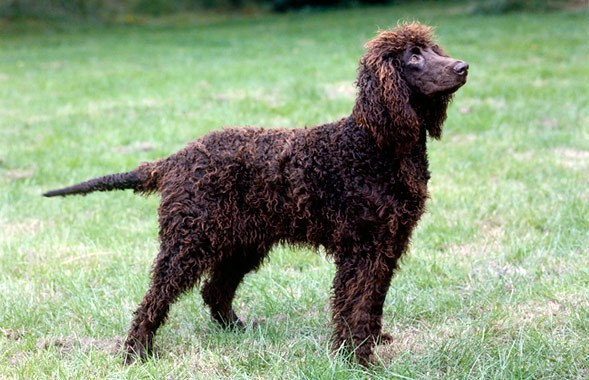
\includegraphics[height=0.5in]{img/water_spaniel} & Irish Spaniel is a Lakeland Terrier with long dark fur and big ears\\
\end{tabular}
}

\ignore{
Once I learn the ``concept'' of a Lakeland Terrier

    \begin{center}
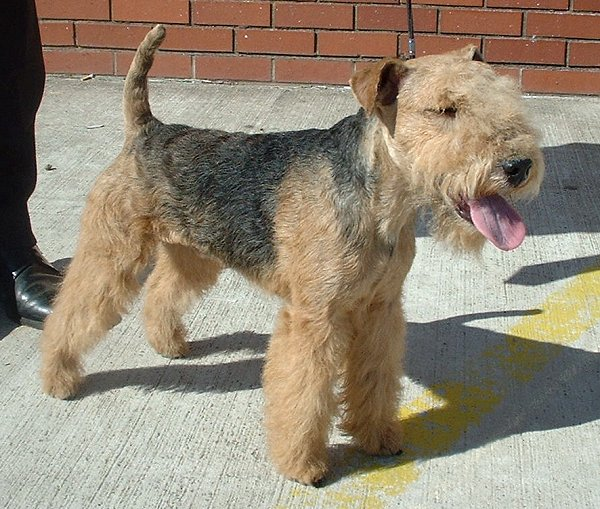
\includegraphics[height=1in]{img/Lakeland_Terrier}
    \end{center}

    \vspace{-0.1in}
    %\pause
I don't have to learn the concept of an Airdale from scratch

    \begin{center}
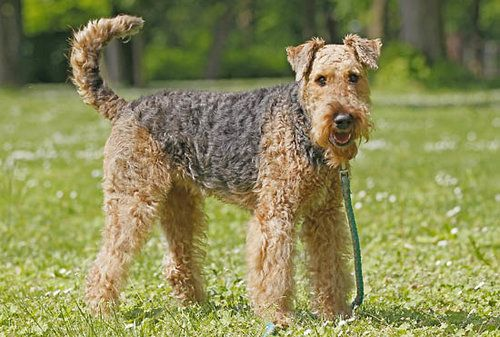
\includegraphics[height=1in]{img/Airedale}
    \end{center}

    \vspace{-0.1in}
I just learn the ``difference'' between these two classes
}

\end{frame}



\begin{frame}
\frametitle{How to build the tree structure?}

\textbf{Goal}: Minimize $\lF{U}$/$\lF{V}$

\vspace{0.1in}
\parbox{10in}{
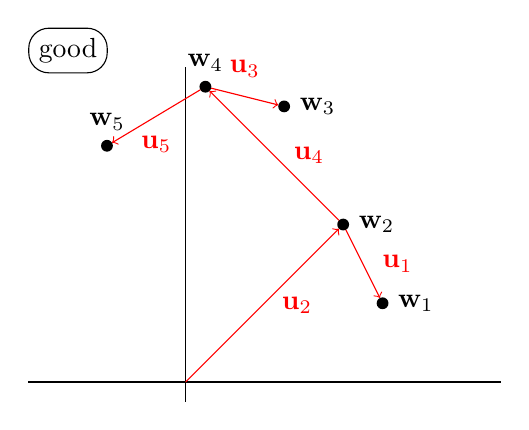
\begin{tikzpicture}
    [
    dot/.style = {minimum width=0.15cm,inner sep=0pt,line width=0pt,fill,circle,black,font=\small}
    ]
\draw[] (0,4) -- (0,-0.25);
\draw[] (4,0) -- (-2,0);
\node[dot,label={0:$\w_1$}] (w1) at (2.5,1) {};
\node[dot,label={0:$\w_2$}] (w2) at (2,2) {};
\node[dot,label={90:$\w_4$}] (w4) at (0.25,3.75) {};
\node[dot,label={0:$\w_3$}] (w3) at (1.25,3.5) {};
\node[dot,label={$\w_5$}] (w5) at (-1,3) {};

\draw[->,color=red] (0,0) -- node[label={0:$\uu_2$}]{} (w2);
\draw[->,color=red] (w2) -- node[label={0:$\uu_1$}]{} (w1);
\draw[->,color=red] (w2) -- node[label={0:$\uu_4$}]{} (w4);
\draw[->,color=red] (w4) -- node[label={$\uu_3$}]{} (w3);
\draw[->,color=red] (w4) -- node[label={270:$\uu_5$}]{} (w5);

\node[anchor=north west, draw, rounded corners=0.1in, inner sep=0.05in] at (-2,4.5) {good};
\end{tikzpicture}
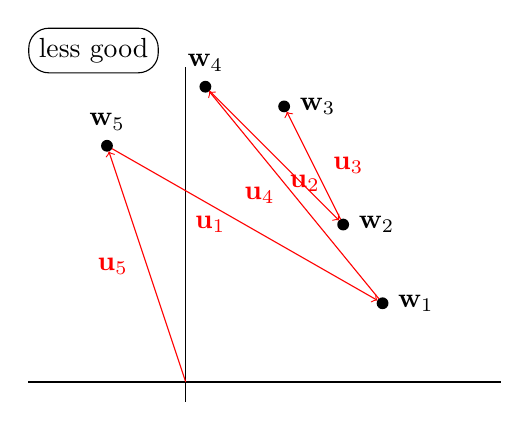
\begin{tikzpicture}
    [
    dot/.style = {minimum width=0.15cm,inner sep=0pt,line width=0pt,fill,circle,black,font=\small}
    ]
\node[anchor=north west, draw, rounded corners=0.1in, inner sep=0.05in] at (-2,4.5) {less good};
\draw[] (0,4) -- (0,-0.25);
\draw[] (4,0) -- (-2,0);
\node[dot,label={0:$\w_1$}] (w1) at (2.5,1) {};
\node[dot,label={0:$\w_2$}] (w2) at (2,2) {};
\node[dot,label={90:$\w_4$}] (w4) at (0.25,3.75) {};
\node[dot,label={0:$\w_3$}] (w3) at (1.25,3.5) {};
\node[dot,label={$\w_5$}] (w5) at (-1,3) {};

\draw[->,color=red] (0,0) -- node[label={180:$\uu_5$}]{} (w5);
\draw[->,color=red] (w5) -- node[label={180:$\uu_1$}]{} (w1);
\draw[->,color=red] (w1) -- node[label={180:$\uu_4$}]{} (w4);
\draw[->,color=red] (w4) -- node[label={300:$\uu_2$}]{} (w2);
\draw[->,color=red] (w2) -- node[label={0:$\uu_3$}]{} (w3);
\end{tikzpicture}
}
\vspace{0.1in}

There's no ``bad'' way to make a tree.

\vspace{0.1in}
\begin{block}{Lemma 2 (informal)}
For all $U$/$V$-tree structures,
%\begin{equation}
$\lF{V} \le \lF{U} \le 2\lF{W} \le 2\sqrt{kd}.$
%\end{equation}
\end{block}

\end{frame}


\begin{frame}
\frametitle{How to build the tree structure? (II)}

Use the \textbf{cover tree} data structure
\begin{itemize}
%\item Build tree over arbitrary metric spaces
\item Good theoretical guarantees
\item I have prior experience with cover trees \citep{izbicki2015faster}
\end{itemize}

%We use the \textbf{cover tree} data structure.

%\begin{block}{Assumption (informal)}
%There exists a distance metric $d$ over the classes that accurately represents
%\end{block}

\vspace{0.1in}
\textbf{Problem:}
\begin{itemize}
\item The tree should be built over the optimal $\w_i^*$ to minimize $\lF{U^*}$/$\lF{V^*}$
\item We don't know $w_i^*$
\end{itemize}

\vspace{0.1in}
\begin{block}{Assumption 3}
    \label{ass:metric}
    Let $\lambda \ge 1$, and $d$ be a distance metric over the labels such that for all labels $i$ and $j$,
\begin{equation}
    \frac 1 \lambda d(i,j)
    \le \ltwo{\star \w_i - \star \w_j}
    \le \lambda d(i, j).
\end{equation}
\end{block}

\end{frame}

\begin{frame}
\frametitle{Main Result!!!}

%\begin{block}{Old Result}
    %\begin{equation}
    %\lF{\star W} \le \sqrt{dk}
    %\end{equation}
%\end{block}


\begin{block}{Lemma 3 (informal)}
Let $c$ be the doubling dimension of the metric in Assumption 3.
Then,
    %Let $c$ be the doubling dimension of the metric in Assumption 3.
    %Then when $c\le1$, we have that
    %\begin{equation}
        %\lF{\star V} \le \lF{\star U} \le \tfrac{1}{\sqrt2}\lambda \sqrt{d\log_2 k} \le \lF{\star W} \le \sqrt{dk},
        %\label{eq:c<=1}
    %\end{equation}
    %and when $c>1$, we have that
    %\begin{equation}
        %\lF{\star V} \le \lF{\star U} \le \sqrt{5}\lambda \sqrt{dk^{(1-1/c)}} \le \lF{\star W} \le \sqrt{dk}.
        %\label{eq:c>1}
    %\end{equation}
\begin{equation}
\lF{\star V} \le \lF{\star U} \le 
O\left(
\begin{cases}
\sqrt{\frac{d \log k}{n}} & c \le 1\\
\sqrt{\frac{d k^{1-1/c}}{n}} & c > 1
\end{cases}
\right)
\le \lF{\star W} \le \sqrt{dk}
\end{equation}
\end{block}

\vspace{0.1in}
Lemmas 1 and 3 immediately imply

\vspace{0.1in}
\begin{block}{Theorem 1 (informal)}
The tree loss satisfies
\begin{equation}
\text{generalization error} \le
O\left(
\begin{cases}
\sqrt{\frac{d \log k}{n}} & c \le 1\\
\sqrt{\frac{d k^{1-1/c}}{n}} & c > 1
\end{cases}
\right)
\le
O\left(\sqrt{\frac{dk}{n}}\right)
\end{equation}
\end{block}

\end{frame}

%%%%%%%%%%%%%%%%%%%%%%%%%%%%%%%%%%%%%%%%%%%%%%%%%%%%%%%%%%%%%%%%%%%%%%%%%%%%%%%%

%\begin{frame}
%\frametitle{What's the doubling dimension $c$?}
%\end{frame}


\begin{frame}{Summary (so far)}

\begin{itemize}
\item more classes $\Rightarrow$ harder problem
\begin{itemize}
\item $k$: num classes, $d$: num dimensions, $n$: num data points
\end{itemize}
\begin{equation*}
\text{(cross entropy) generalization error}
=
O\left(\sqrt{\frac{kd}{n}}\right)
~~~~~~~~~~
\end{equation*}
\item real world classes are highly structured

\begin{itemize}
\item the doubling dimension $c <\!\!< k$

\end{itemize}
\begin{equation*}
\text{(conjectured optimal) generalization error}
=
O\left(\sqrt{\frac{cd}{n}}\right)
~~~~~~~~~~~~~~~~~~~~~~~~~~~~~~.
\end{equation*}

\item \textbf{contribution:} $U$/$V$-tree loss exploits arbitrary metric structure

\begin{equation*}
\text{(tree loss) generalization error} = 
\begin{cases}
\sqrt{\frac{d\log k}{n}} & c\le 1 \\
\sqrt{\frac{dk^{1-1/c}}{n}} & c>1 \\
\end{cases}
\end{equation*}

\item \textbf{bonus:} best performance on synthetic and real world experiments

\end{itemize}

\vspace{-4in}
\begin{tikzpicture}
    \node at (0,0) {};
    \node at (0,4in) {};

    %\node[anchor=north west,fill=white,minimum width=4.5in,minimum height=0.7in] at (0,2.94in) {};
    %\node[anchor=north west,fill=white,minimum width=4.5in,minimum height=0.74in] at (0,2.04in) {};
    %\node[anchor=north west,fill=white,minimum width=4.5in,minimum height=0.7in] at (0,1.04in) {};
    \node[anchor=north west,fill=white,minimum width=4.5in,minimum height=0.3in] at (0,0.3in) {};
\end{tikzpicture}
\end{frame}




\begin{frame}
\frametitle{(Content Warning) Proof Culture in Machine Learning}
\pause
\begin{tikzpicture}
\node at (0,0) {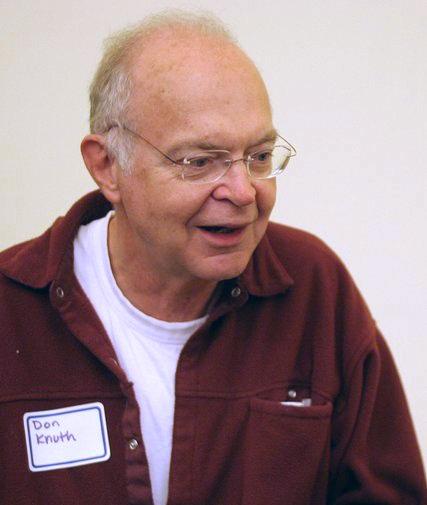
\includegraphics[width=2in]{img/knuth}};
\node at (6,0) {\parbox{2.4in}{
    \Large
Beware of bugs in the above code; I have only proved it correct, not tried it.

\vspace{0.2in}
-- Donald Knuth
}};
\end{tikzpicture}
\end{frame}

%%%%%%%%%%%%%%%%%%%%%%%%%%%%%%%%%%%%%%%%%%%%%%%%%%%%%%%%%%%%%%%%%%%%%%%%%%%%%%%%

\begin{frame}
\frametitle{(Content Warning) Proof Culture in Machine Learning}

Google Scholar's most cited paper of 2020:\footnote{
    \tiny\url{https://www.natureindex.com/news-blog/google-scholar-reveals-most-influential-papers-research-citations-twenty-twenty}
}

\vspace{0.1in}

\includegraphics[width=\textwidth]{img/adam}

\pause
\citet{reddi2019convergence}
\begin{itemize}
\item
    Simple counter example to Adam paper's proofs
\item
    Provide a fixed, corrected algorithm AdamW
\item
    ``Only'' 1500 citations
\item
    Adam paper has $>60000$ citations since \citet{reddi2019convergence} published
\end{itemize}
\end{frame}

%%%%%%%%%%%%%%%%%%%%%%%%%%%%%%%%%%%%%%%%%%%%%%%%%%%%%%%%%%%%%%%%%%%%%%%%%%%%%%%%

\begin{frame}
\frametitle{(Content Warning) Proof Culture in Machine Learning}

\begin{tikzpicture}
\node at (0,0) {
\includegraphics[width=2in]{img/facebookanon}};
\node at (6,0) {\parbox{2.4in}{
\begin{flushleft}
\Large
I don't care about theorems or proofs.
I only look at the experiments.

\vspace{0.2in}
-- Reviewer \#3
\end{flushleft}
}};

%\pause
    %\draw[red, line width=2pt] (3,0) -- (5.5,0);
    %\node at (7,-0.1) {\Large\color{red} cute animals};
\end{tikzpicture}

\end{frame}

\begin{frame}{Summary (so far)}

\begin{itemize}
\item more classes $\Rightarrow$ harder problem
\begin{itemize}
\item $k$: num classes, $d$: num dimensions, $n$: num data points
\end{itemize}
\begin{equation*}
\text{(cross entropy) generalization error}
=
O\left(\sqrt{\frac{kd}{n}}\right)
~~~~~~~~~~
\end{equation*}
\item real world classes are highly structured

\begin{itemize}
\item the doubling dimension $c <\!\!< k$

\end{itemize}
\begin{equation*}
\text{(conjectured optimal) generalization error}
=
O\left(\sqrt{\frac{cd}{n}}\right)
~~~~~~~~~~~~~~~~~~~~~~~~~~~~~~.
\end{equation*}

\item \textbf{contribution:} $U$/$V$-tree loss exploits arbitrary metric structure

\begin{equation*}
\text{(tree loss) generalization error} = 
\begin{cases}
\sqrt{\frac{d\log k}{n}} & c\le 1 \\
\sqrt{\frac{dk^{1-1/c}}{n}} & c>1 \\
\end{cases}
\end{equation*}

\item \textbf{bonus:} best performance on synthetic and real world experiments

\end{itemize}

\vspace{-4in}
\begin{tikzpicture}
    \node at (0,0) {};
    \node at (0,4in) {};

    %\node[anchor=north west,fill=white,minimum width=4.5in,minimum height=0.7in] at (0,2.94in) {};
    %\node[anchor=north west,fill=white,minimum width=4.5in,minimum height=0.74in] at (0,2.04in) {};
    %\node[anchor=north west,fill=white,minimum width=4.5in,minimum height=0.7in] at (0,1.04in) {};
    %\node[anchor=north west,fill=white,minimum width=4.5in,minimum height=0.3in] at (0,0.3in) {};
\end{tikzpicture}
\end{frame}





\makeatletter
\tikzset{
  base/.is choice,
  base/top/.code={\let\vbox\vtop},
  base/bottom/.code={\def\pgfutil@minipage[t]{\minipage[b]}},
  % base/bottom/.code={}, % for plain TeX
}
\makeatother

%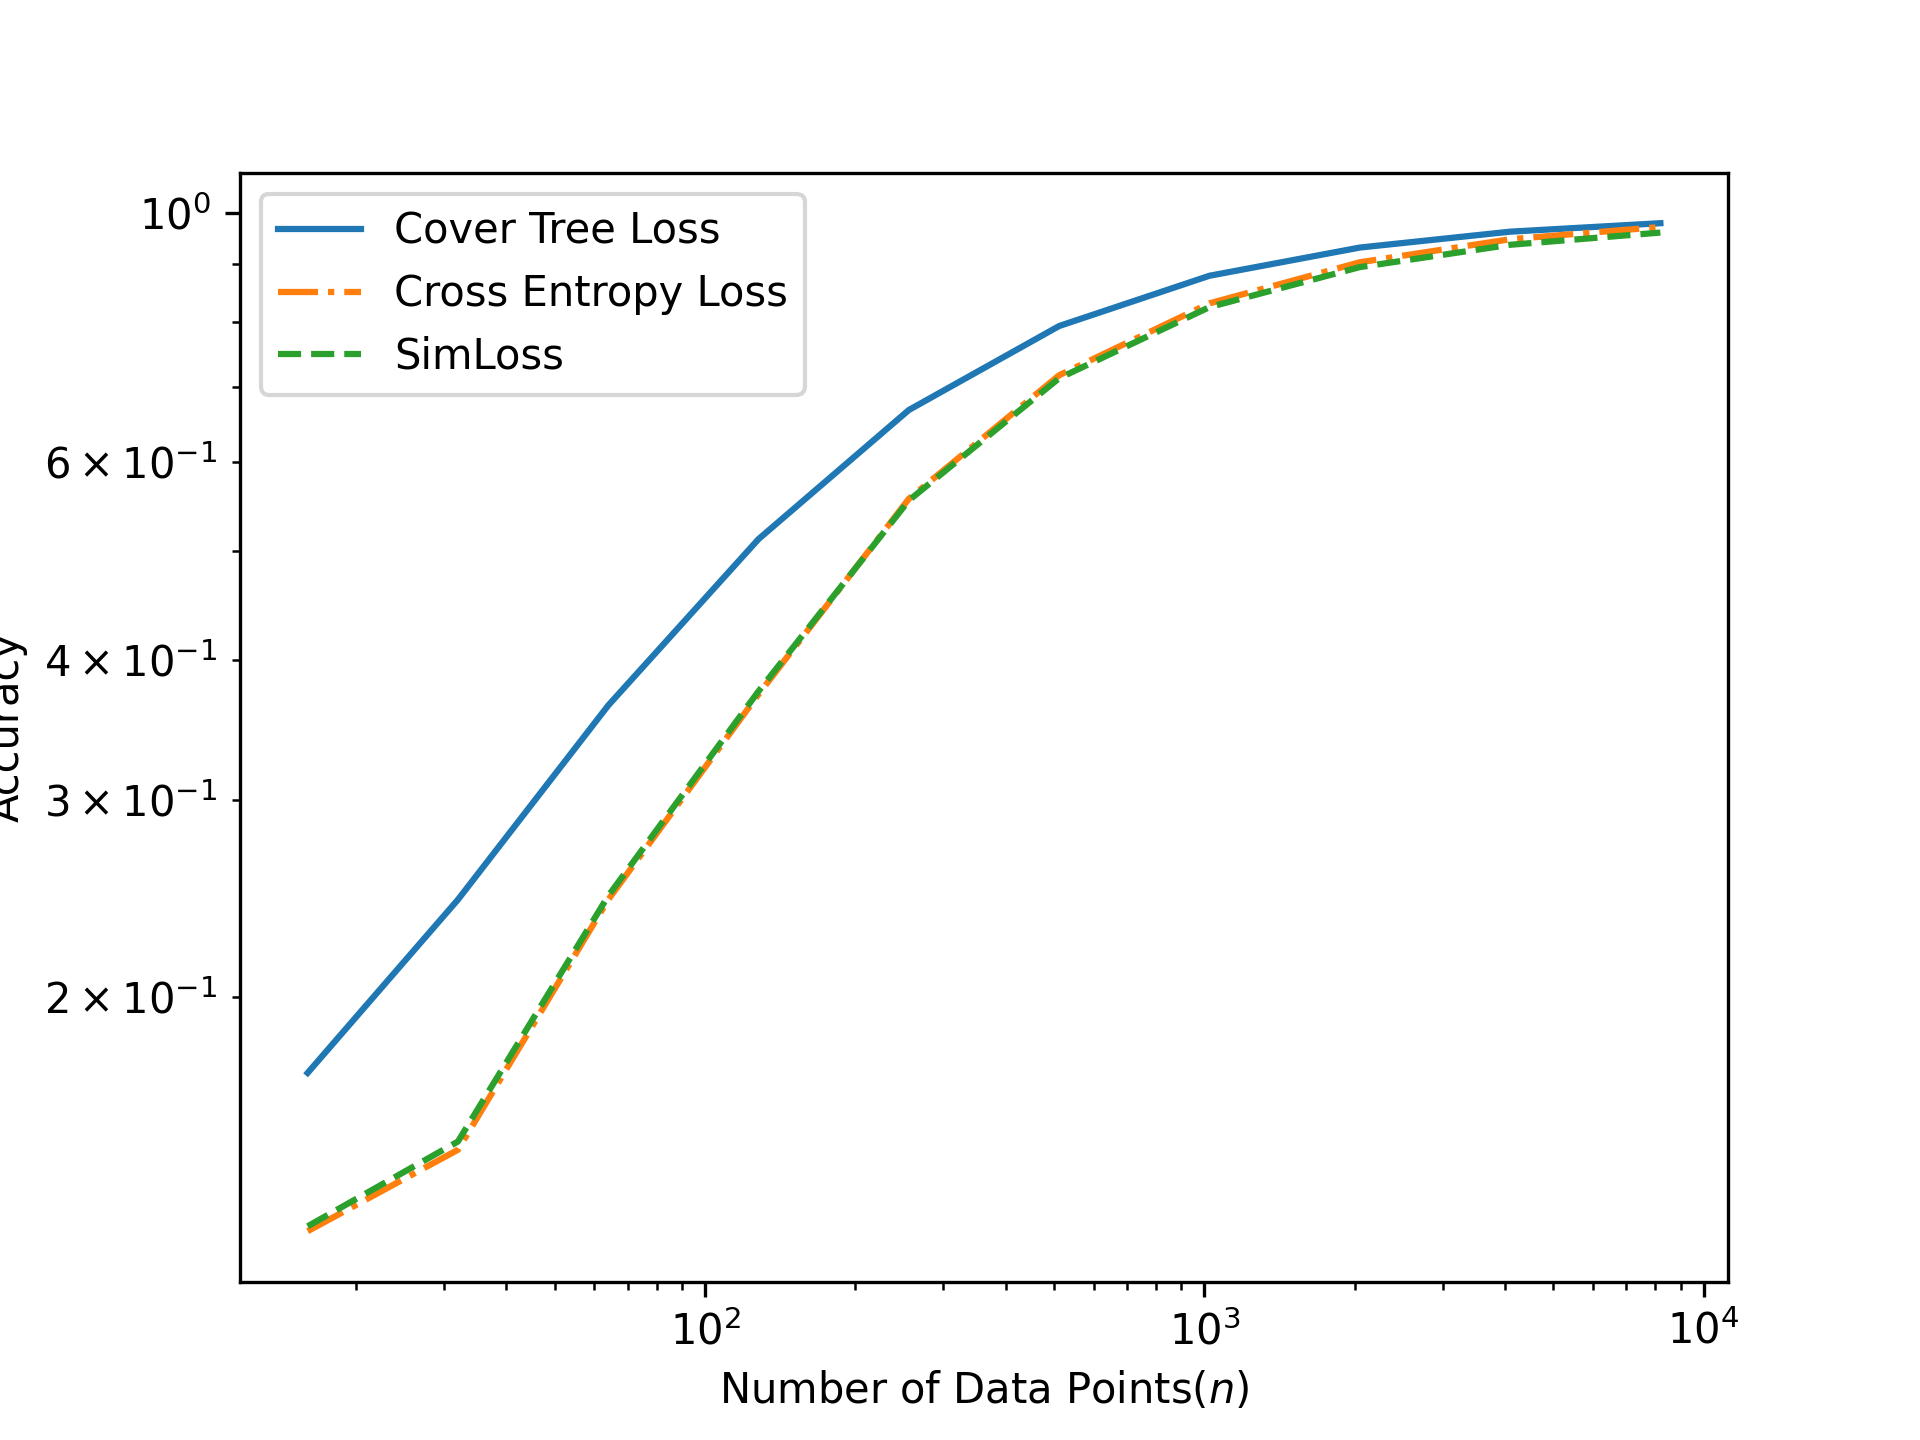
\includegraphics[width=0.48\columnwidth]{fig/images/accuracy_vs_n.png}
%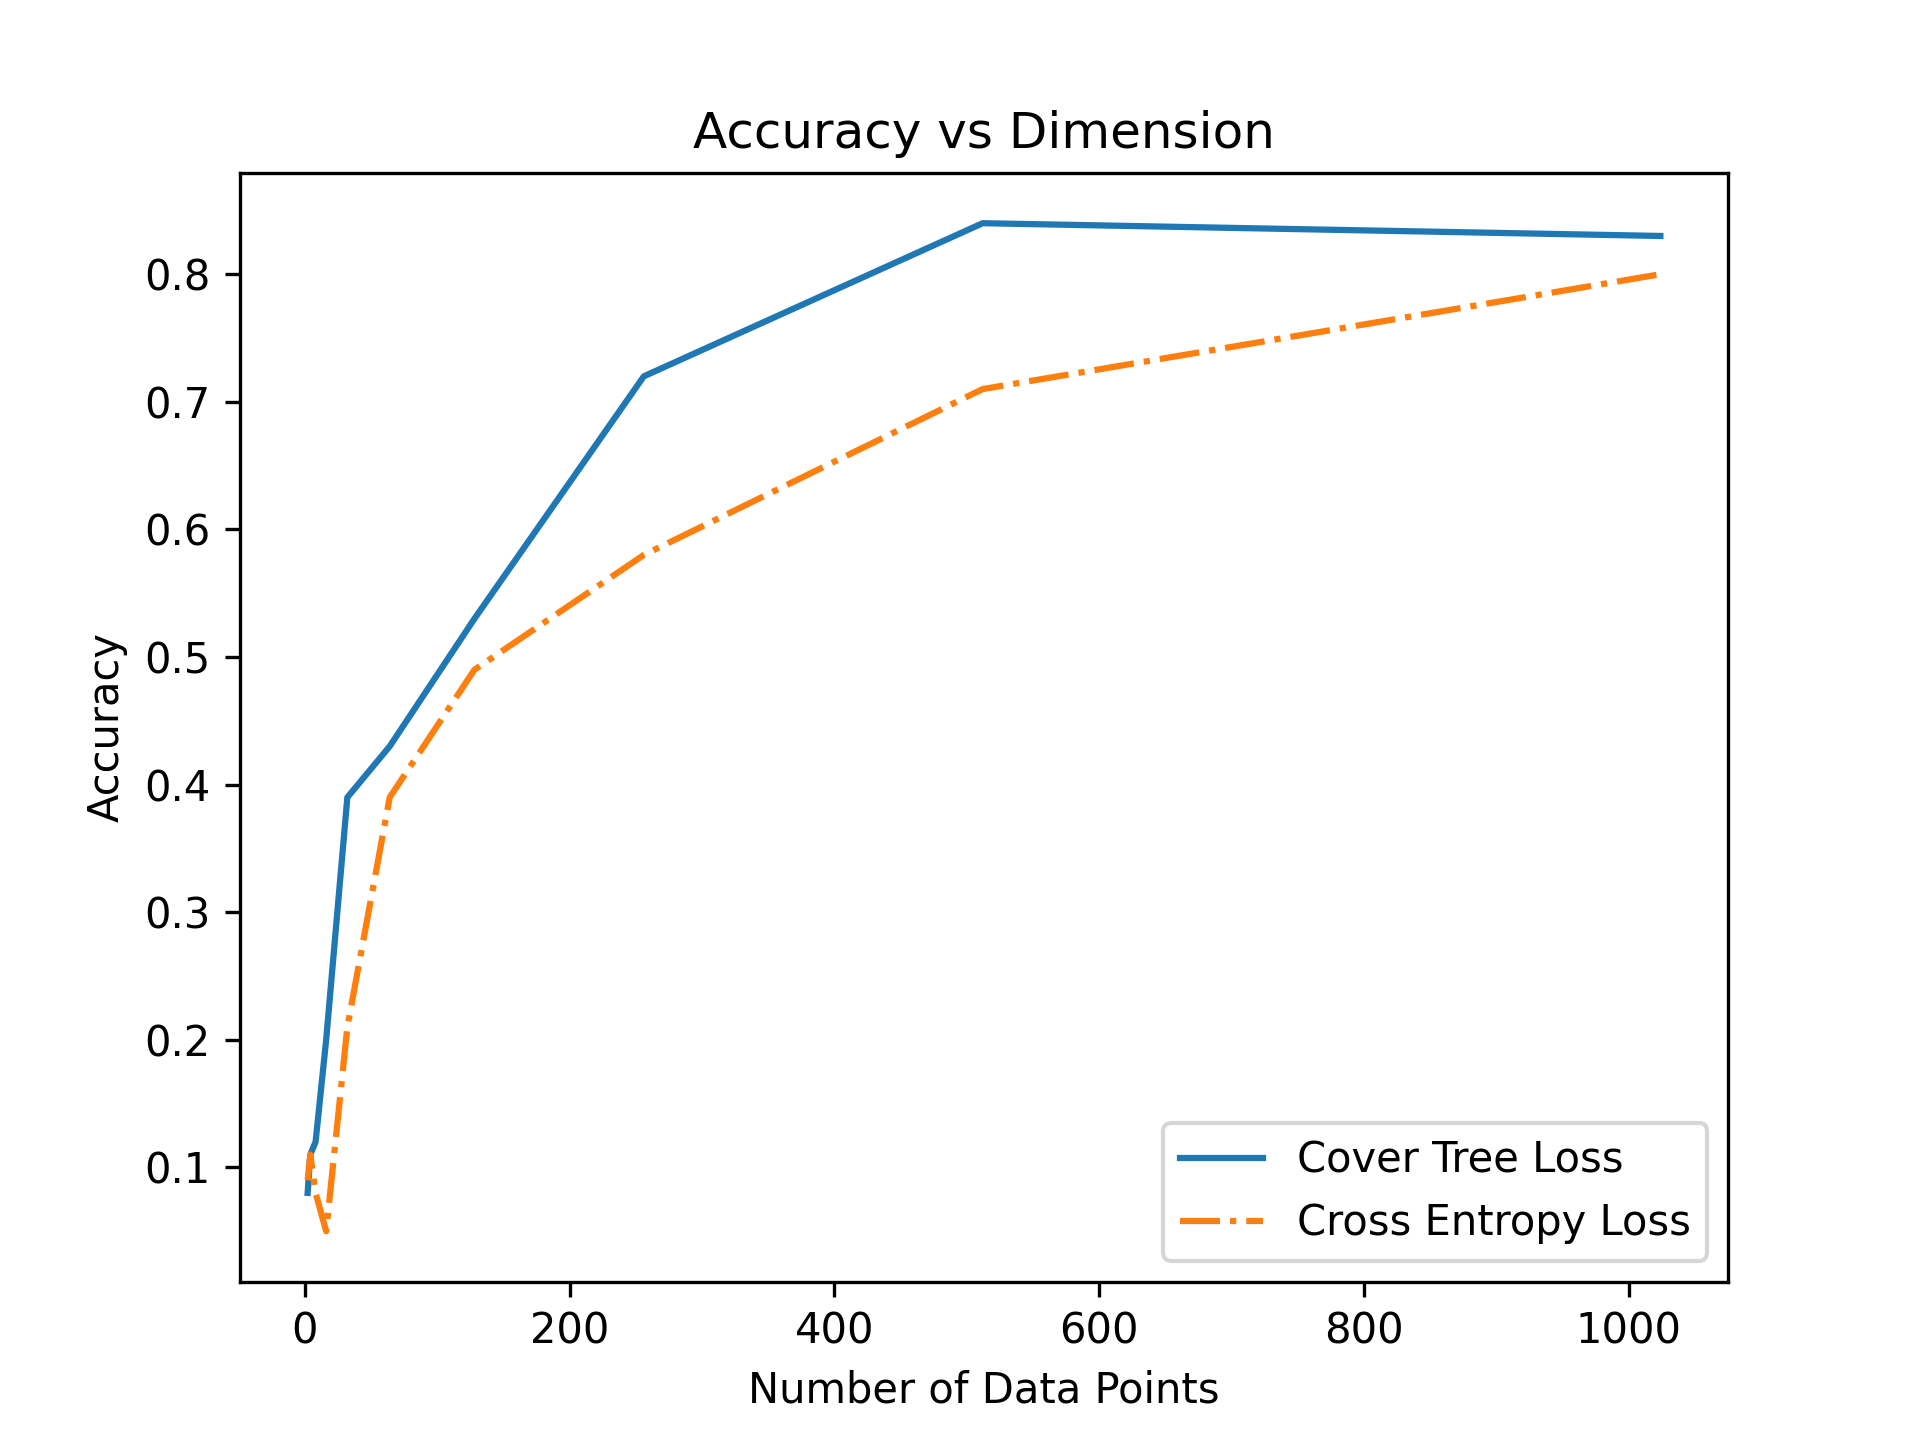
\includegraphics[width=0.48\columnwidth]{fig/images/accuracy_vs_d.png}
%
%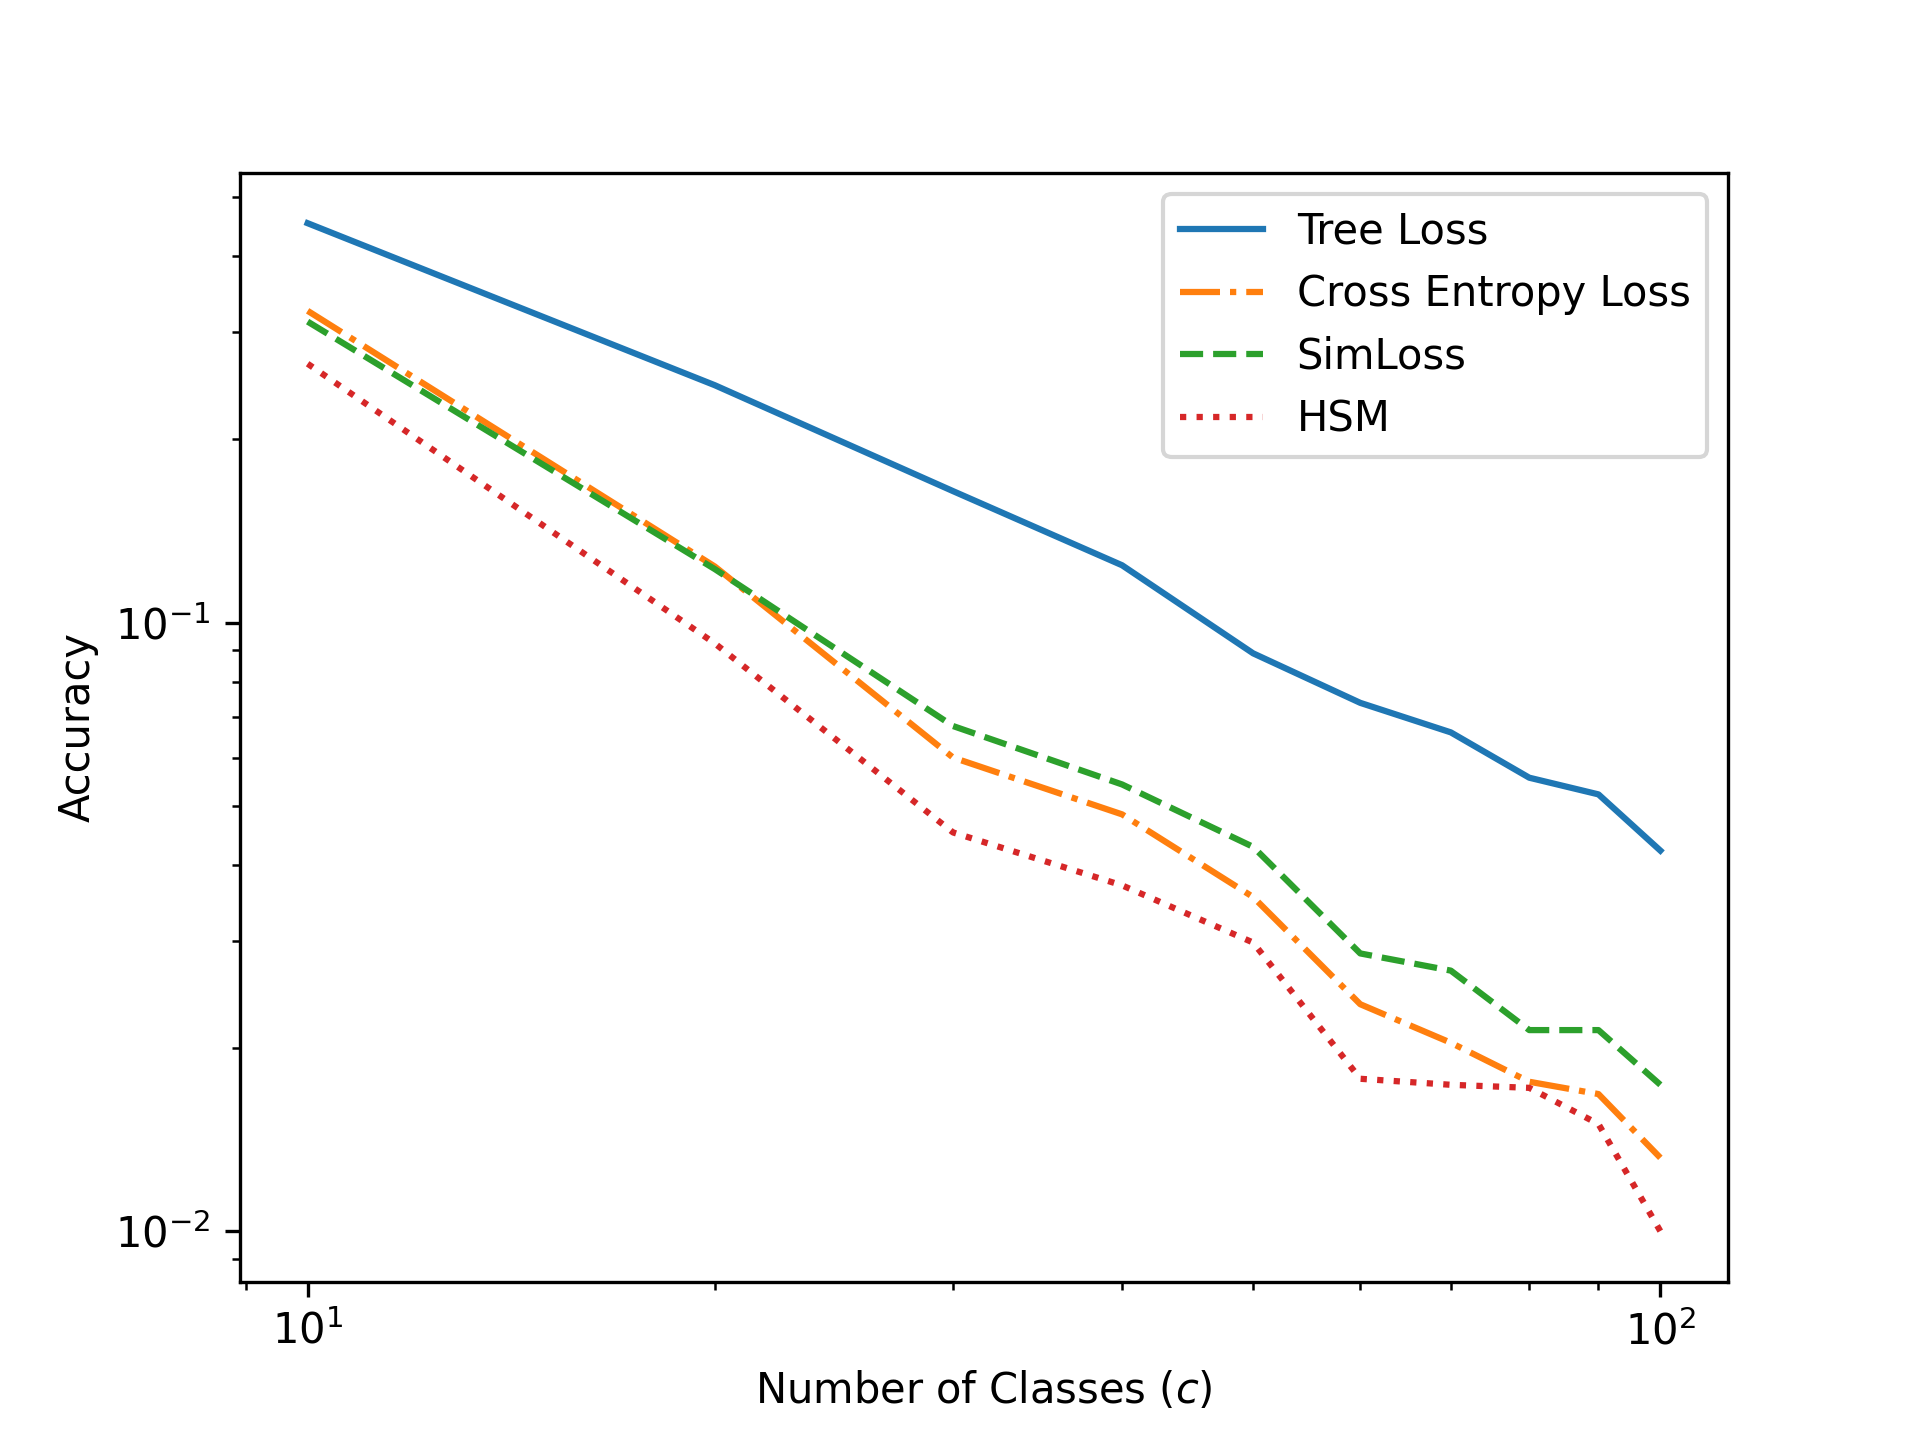
\includegraphics[width=0.48\columnwidth]{fig/images/accuracy_vs_class.png}
%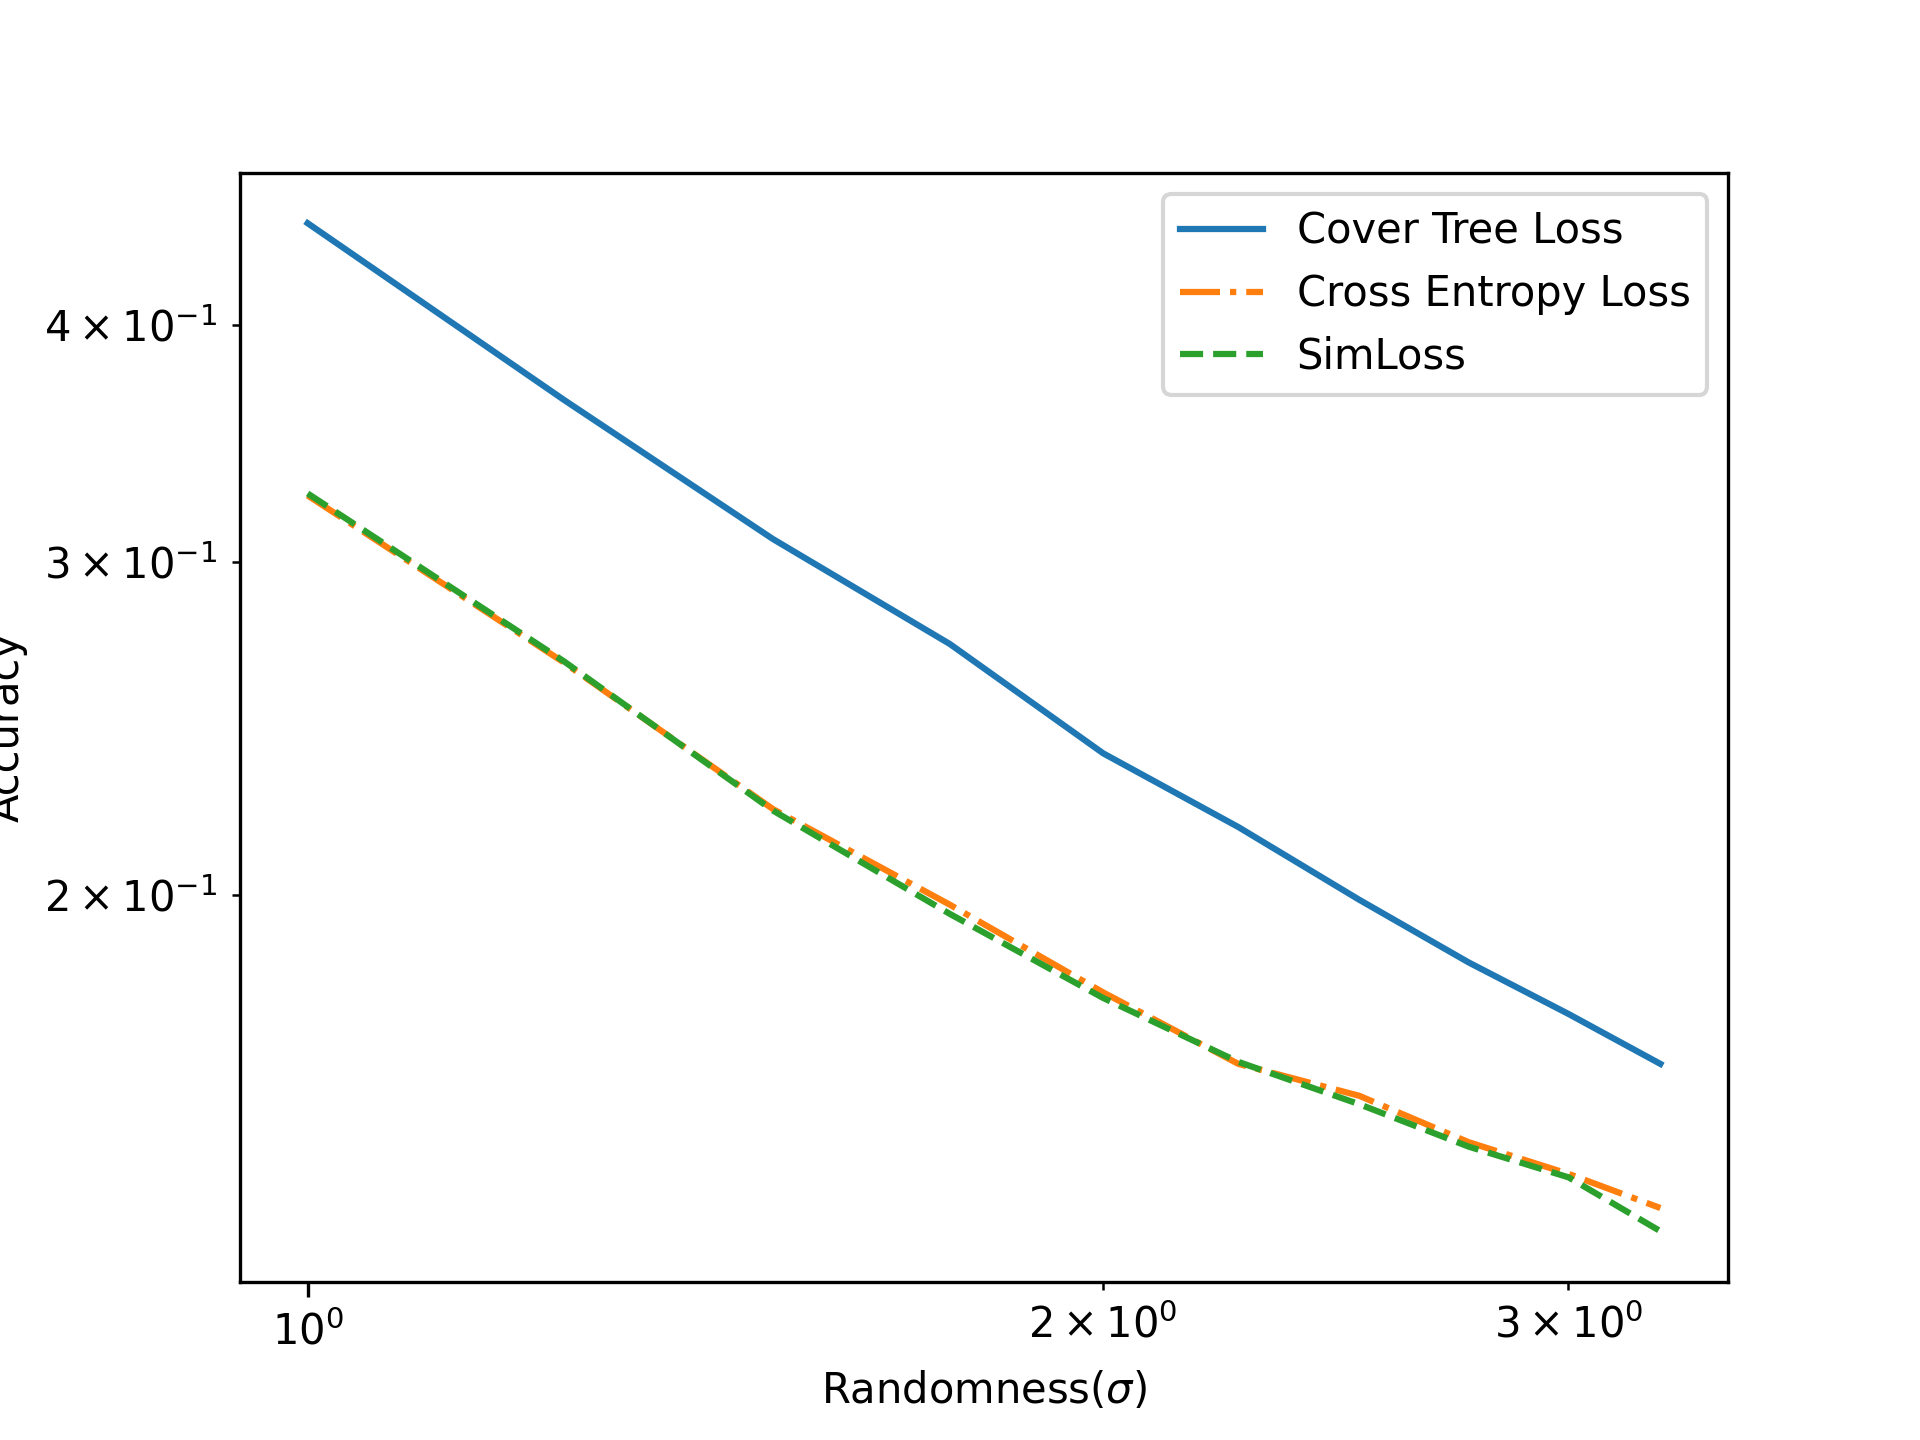
\includegraphics[width=0.48\columnwidth]{fig/images/accuracy_vs_sigma.png}

%%%%%%%%%%%%%%%%%%%%%%%%%%%%%%%%%%%%%%%%%%%%%%%%%%%%%%%%%%%%%%%%%%%%%%%%%%%%%%%%

\begin{frame}{Experiments: Synthetic: Ablation}
\begin{center}
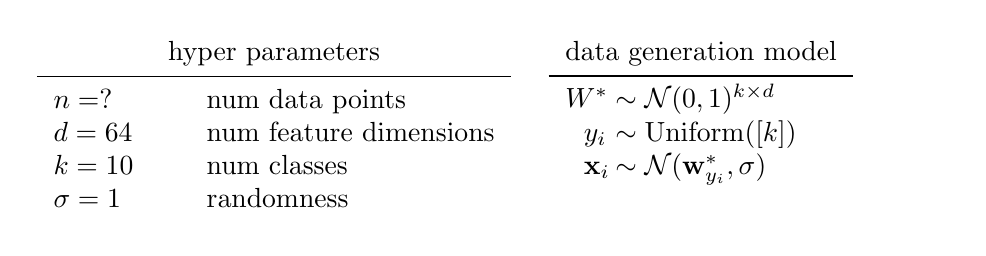
\begin{tikzpicture}
    \node[minimum height=1in]{\parbox{2in}{
        \begin{tabular}{p{0.6in}l}
            \multicolumn{2}{c}{hyper parameters} \\
            \midrule
            $n=?$ & num data points \\
            $d=64$ & num feature dimensions \\
            $k=10$ & num classes \\
            $\sigma=1$ & randomness \\
        \end{tabular}
    }};
    \node[minimum height=1in] at (6.5,0) {\parbox{2in}{
        \begin{tabular}{ll}
            \multicolumn{2}{c}{data generation model} \\
            \midrule
            $W^*$ & \!\!\!\!\!\!$\sim \mathcal N(0,1)^{k\times d}$ \\
            ~~$y_i$ & \!\!\!\!\!\!$\sim \text{Uniform}([k])$ \\
            ~~$\x_i$ & \!\!\!\!\!\!$\sim \mathcal N(\w^*_{y_i}, \sigma)$ \\
            \\
        \end{tabular}
    }};
\end{tikzpicture}
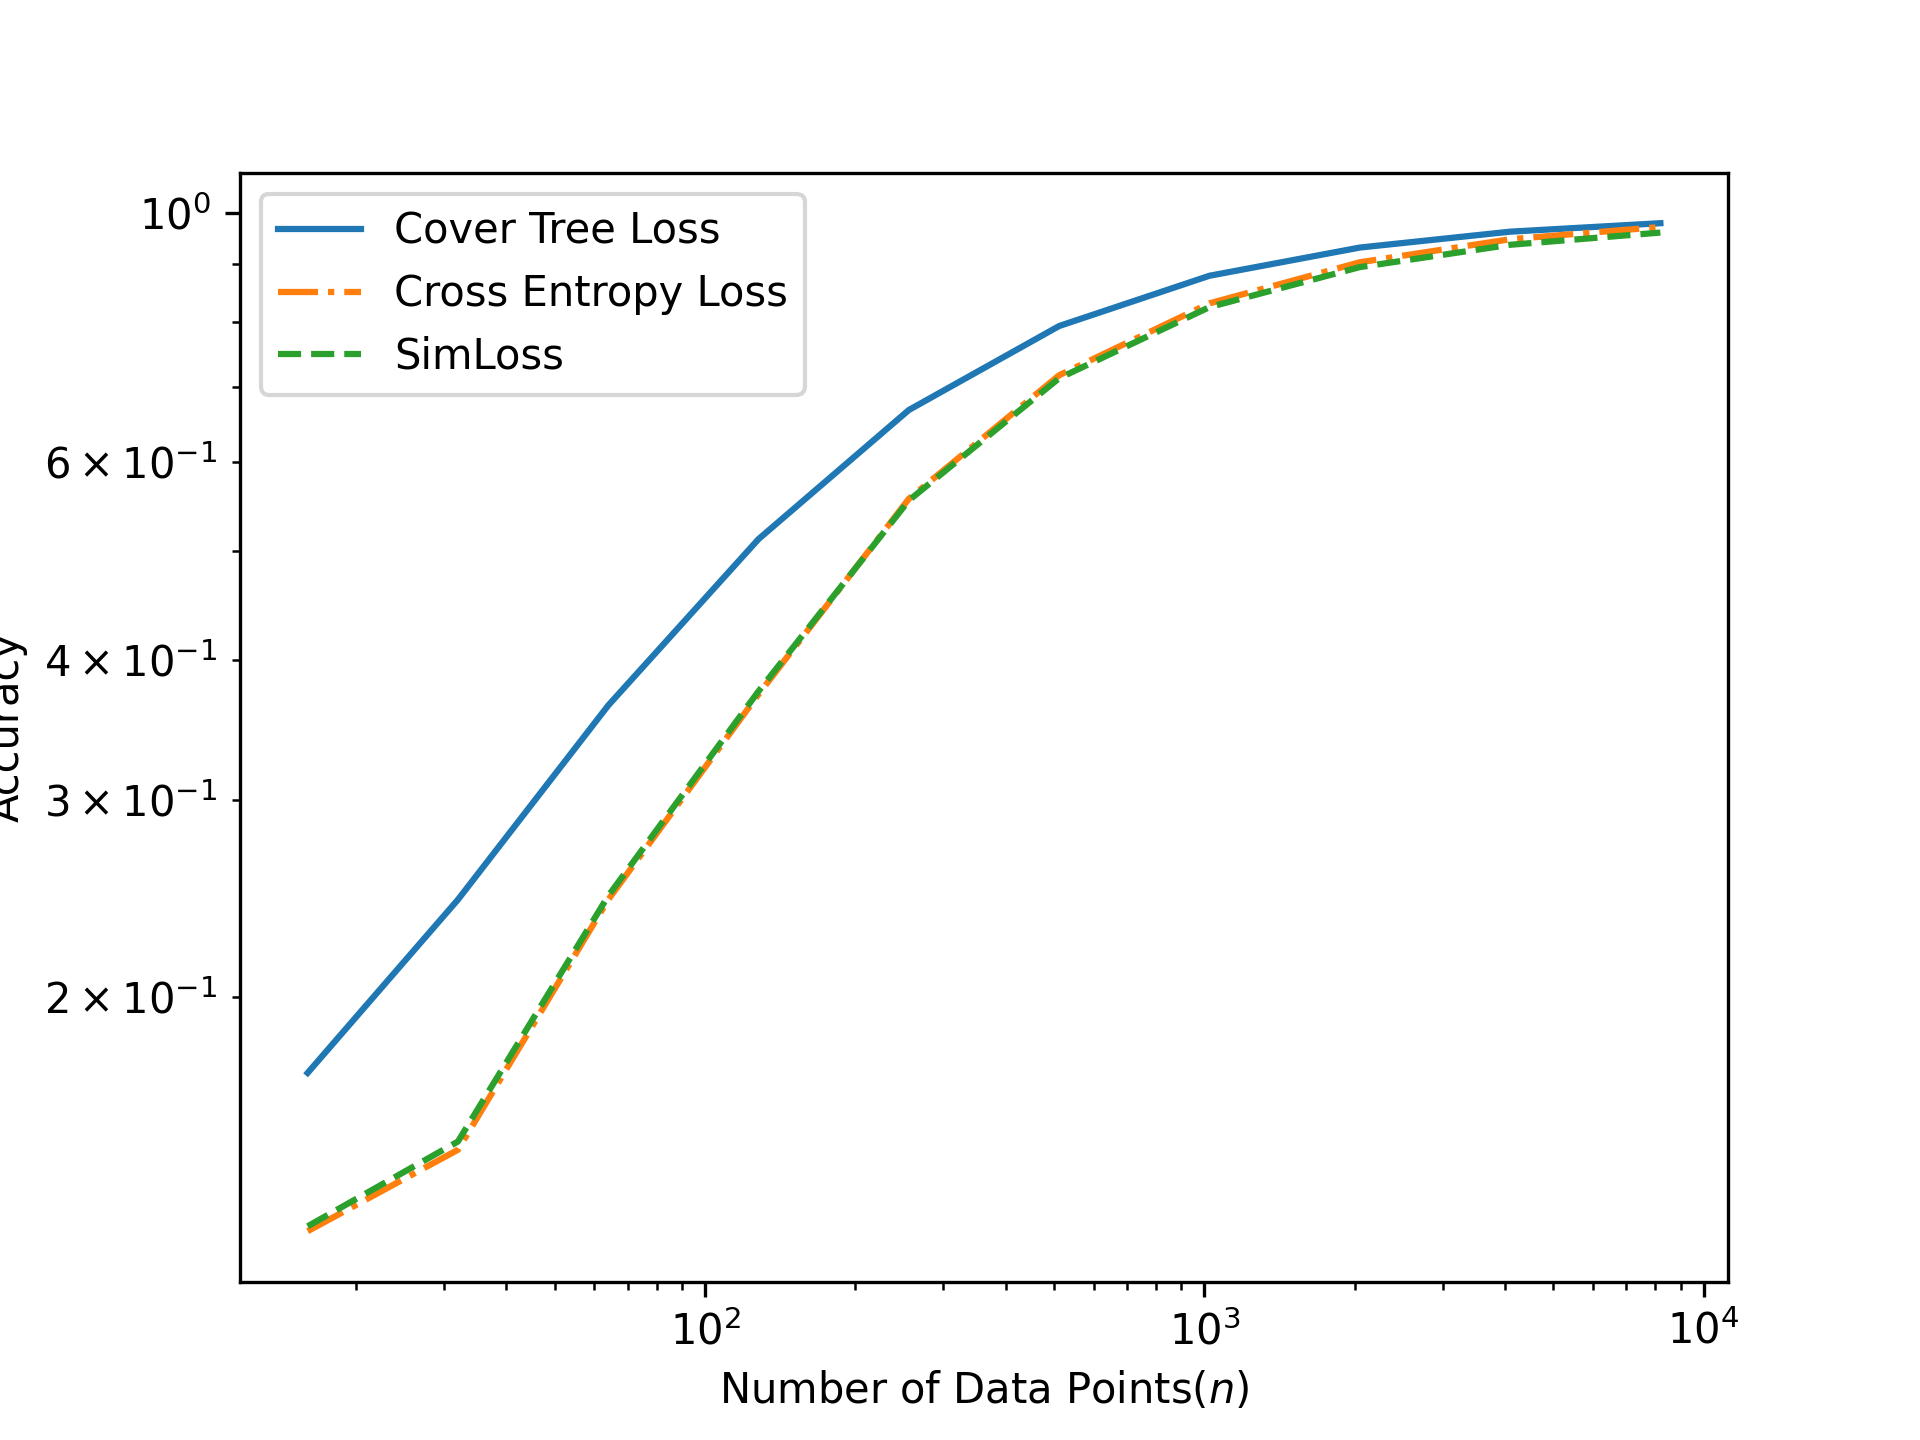
\includegraphics[width=0.8\columnwidth]{fig/images/accuracy_vs_n.png}
\end{center}
\end{frame}

%%%%%%%%%%%%%%%%%%%%

\begin{frame}{Experiments: Synthetic: Ablation}
\begin{center}
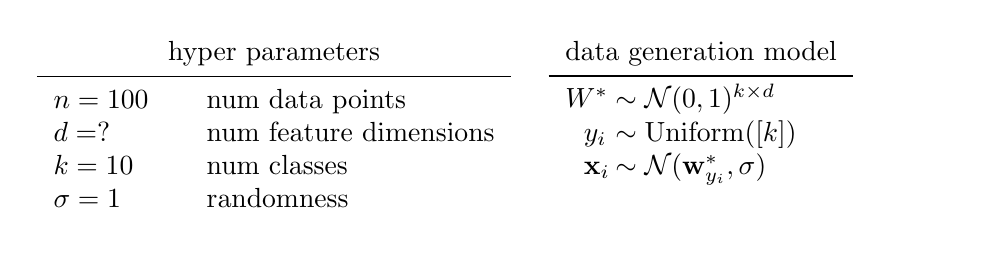
\begin{tikzpicture}
    \node[minimum height=1in]{\parbox{2in}{
        \begin{tabular}{p{0.6in}l}
            \multicolumn{2}{c}{hyper parameters} \\
            \midrule
            $n=100$ & num data points \\
            $d=?$ & num feature dimensions \\
            $k=10$ & num classes \\
            $\sigma=1$ & randomness \\
        \end{tabular}
    }};
    \node[minimum height=1in] at (6.5,0) {\parbox{2in}{
        \begin{tabular}{ll}
            \multicolumn{2}{c}{data generation model} \\
            \midrule
            $W^*$ & \!\!\!\!\!\!$\sim \mathcal N(0,1)^{k\times d}$ \\
            ~~$y_i$ & \!\!\!\!\!\!$\sim \text{Uniform}([k])$ \\
            ~~$\x_i$ & \!\!\!\!\!\!$\sim \mathcal N(\w^*_{y_i}, \sigma)$ \\
            \\
        \end{tabular}
    }};
\end{tikzpicture}
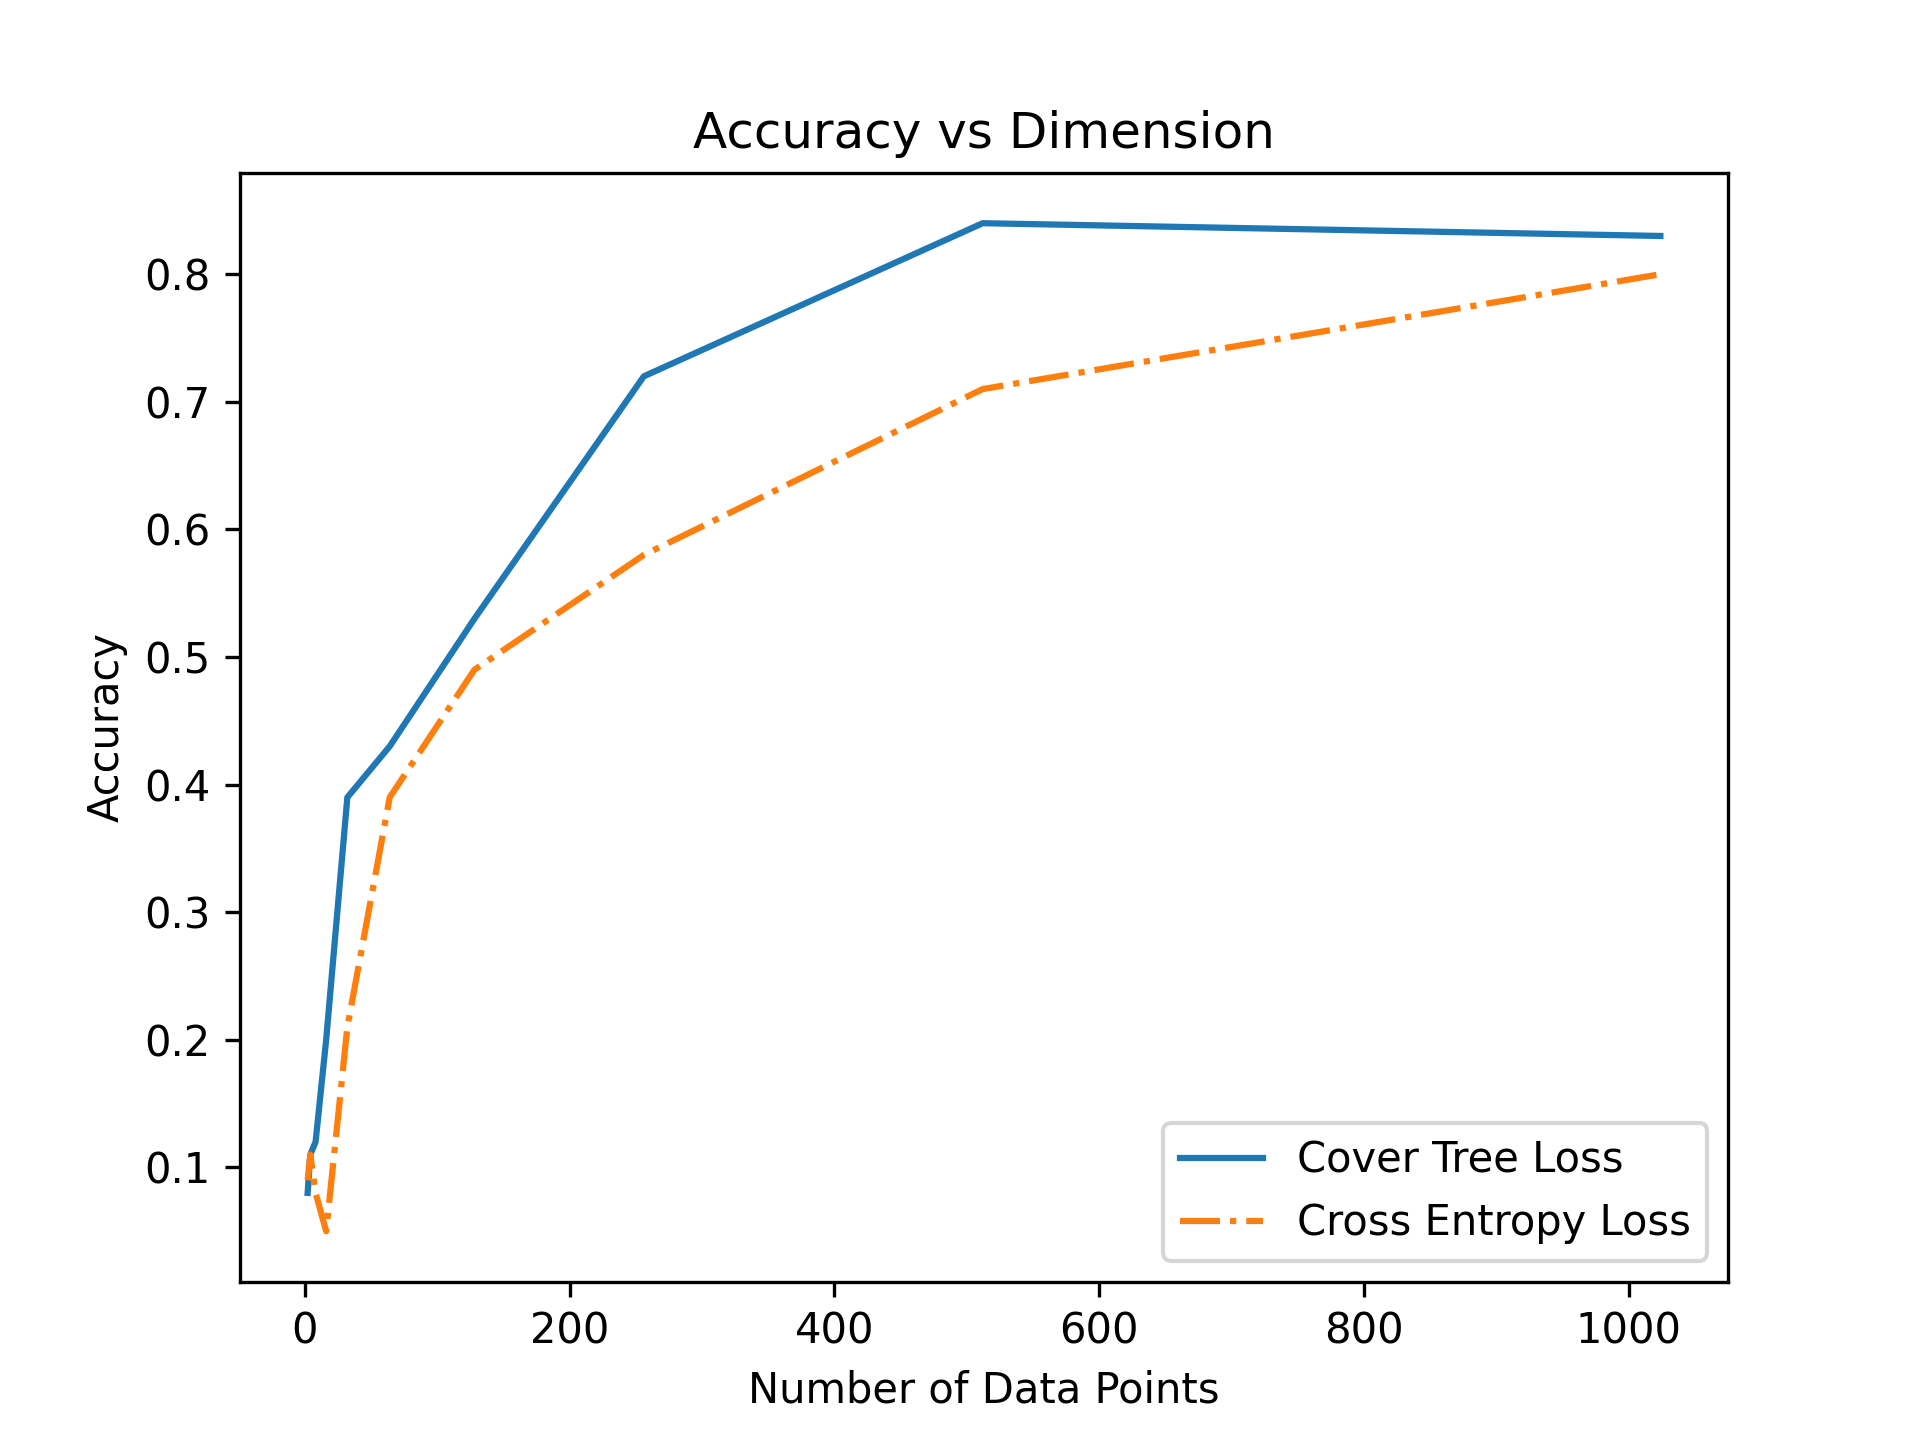
\includegraphics[width=0.8\columnwidth]{fig/images/accuracy_vs_d.png}
\end{center}
\end{frame}

%%%%%%%%%%%%%%%%%%%%

\begin{frame}{Experiments: Synthetic: Ablation}
\begin{center}
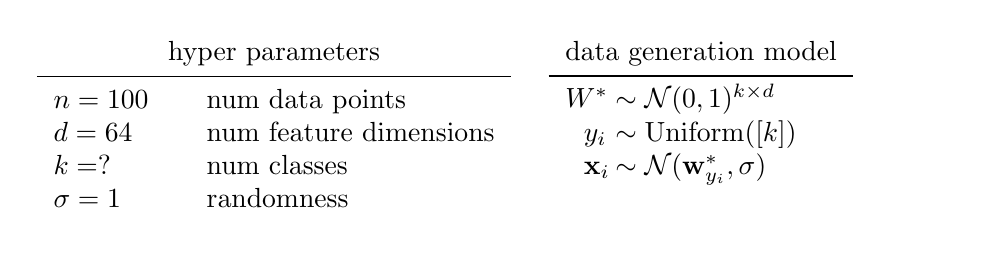
\begin{tikzpicture}
    \node[minimum height=1in]{\parbox{2in}{
        \begin{tabular}{p{0.6in}l}
            \multicolumn{2}{c}{hyper parameters} \\
            \midrule
            $n=100$ & num data points \\
            $d=64$ & num feature dimensions \\
            $k=?$ & num classes \\
            $\sigma=1$ & randomness \\
        \end{tabular}
    }};
    \node[minimum height=1in] at (6.5,0) {\parbox{2in}{
        \begin{tabular}{ll}
            \multicolumn{2}{c}{data generation model} \\
            \midrule
            $W^*$ & \!\!\!\!\!\!$\sim \mathcal N(0,1)^{k\times d}$ \\
            ~~$y_i$ & \!\!\!\!\!\!$\sim \text{Uniform}([k])$ \\
            ~~$\x_i$ & \!\!\!\!\!\!$\sim \mathcal N(\w^*_{y_i}, \sigma)$ \\
            \\
        \end{tabular}
    }};
\end{tikzpicture}
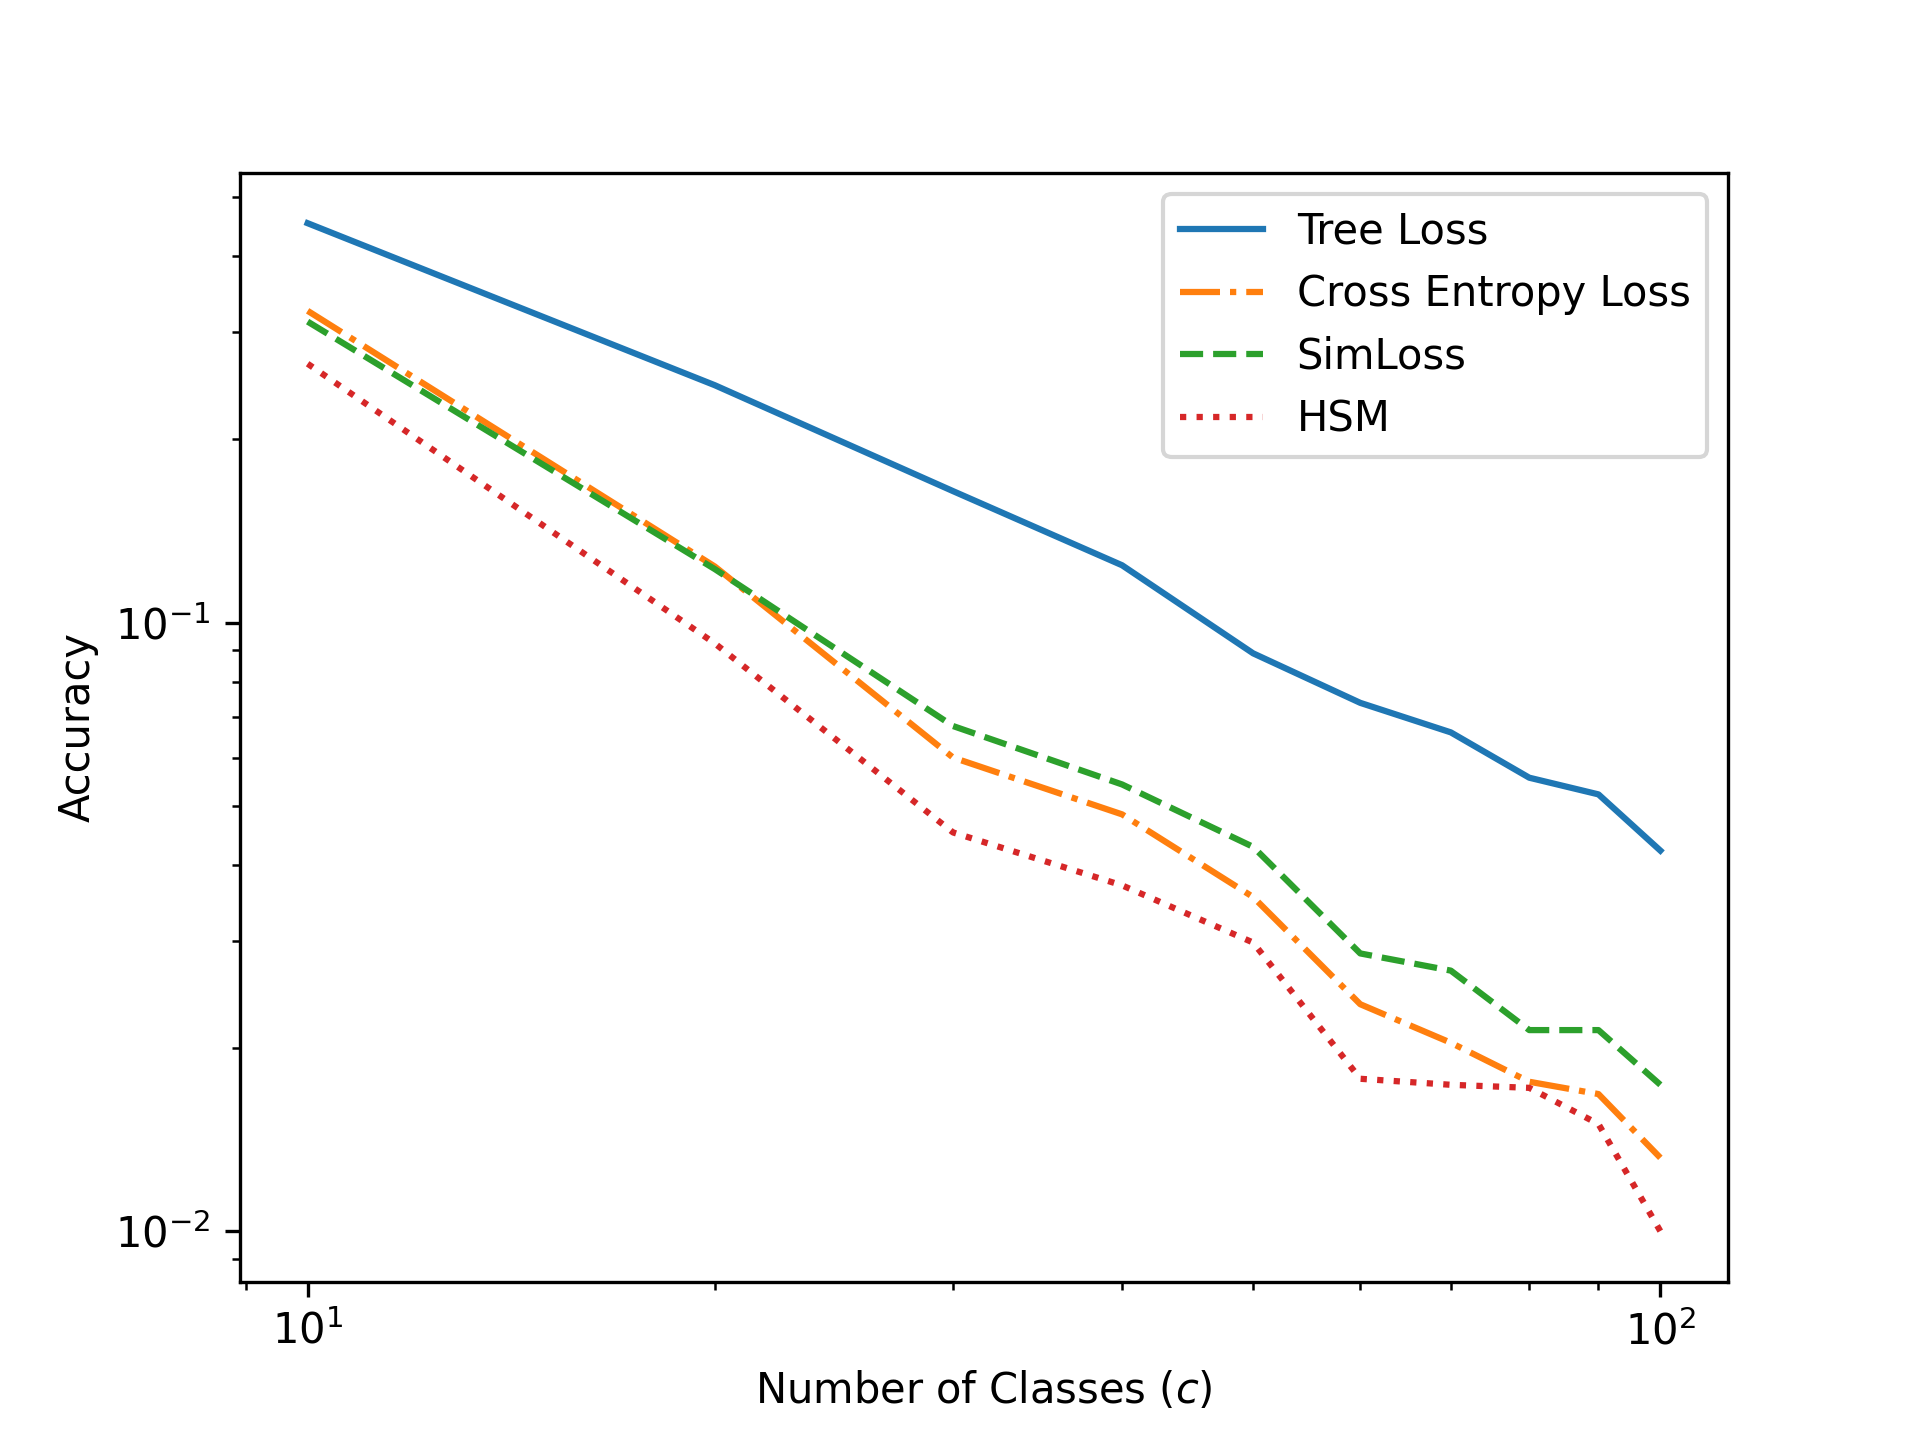
\includegraphics[width=0.8\columnwidth]{fig/images/accuracy_vs_class.png}
\end{center}
\end{frame}

%%%%%%%%%%%%%%%%%%%%

\begin{frame}{Experiments: Synthetic: Ablation}
\begin{center}
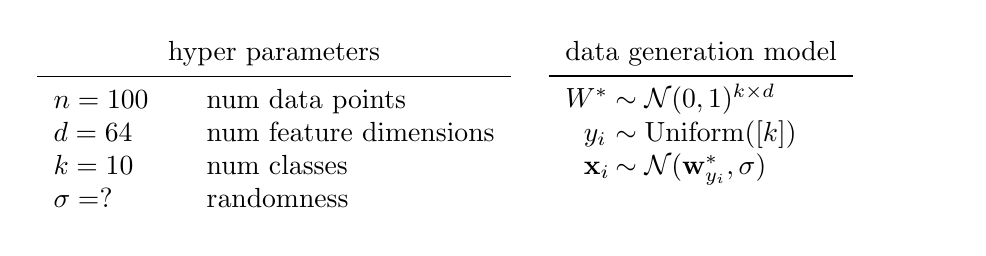
\begin{tikzpicture}
    \node[minimum height=1in]{\parbox{2in}{
        \begin{tabular}{p{0.6in}l}
            \multicolumn{2}{c}{hyper parameters} \\
            \midrule
            $n=100$ & num data points \\
            $d=64$ & num feature dimensions \\
            $k=10$ & num classes \\
            $\sigma=?$ & randomness \\
        \end{tabular}
    }};
    \node[minimum height=1in] at (6.5,0) {\parbox{2in}{
        \begin{tabular}{ll}
            \multicolumn{2}{c}{data generation model} \\
            \midrule
            $W^*$ & \!\!\!\!\!\!$\sim \mathcal N(0,1)^{k\times d}$ \\
            ~~$y_i$ & \!\!\!\!\!\!$\sim \text{Uniform}([k])$ \\
            ~~$\x_i$ & \!\!\!\!\!\!$\sim \mathcal N(\w^*_{y_i}, \sigma)$ \\
            \\
        \end{tabular}
    }};
\end{tikzpicture}
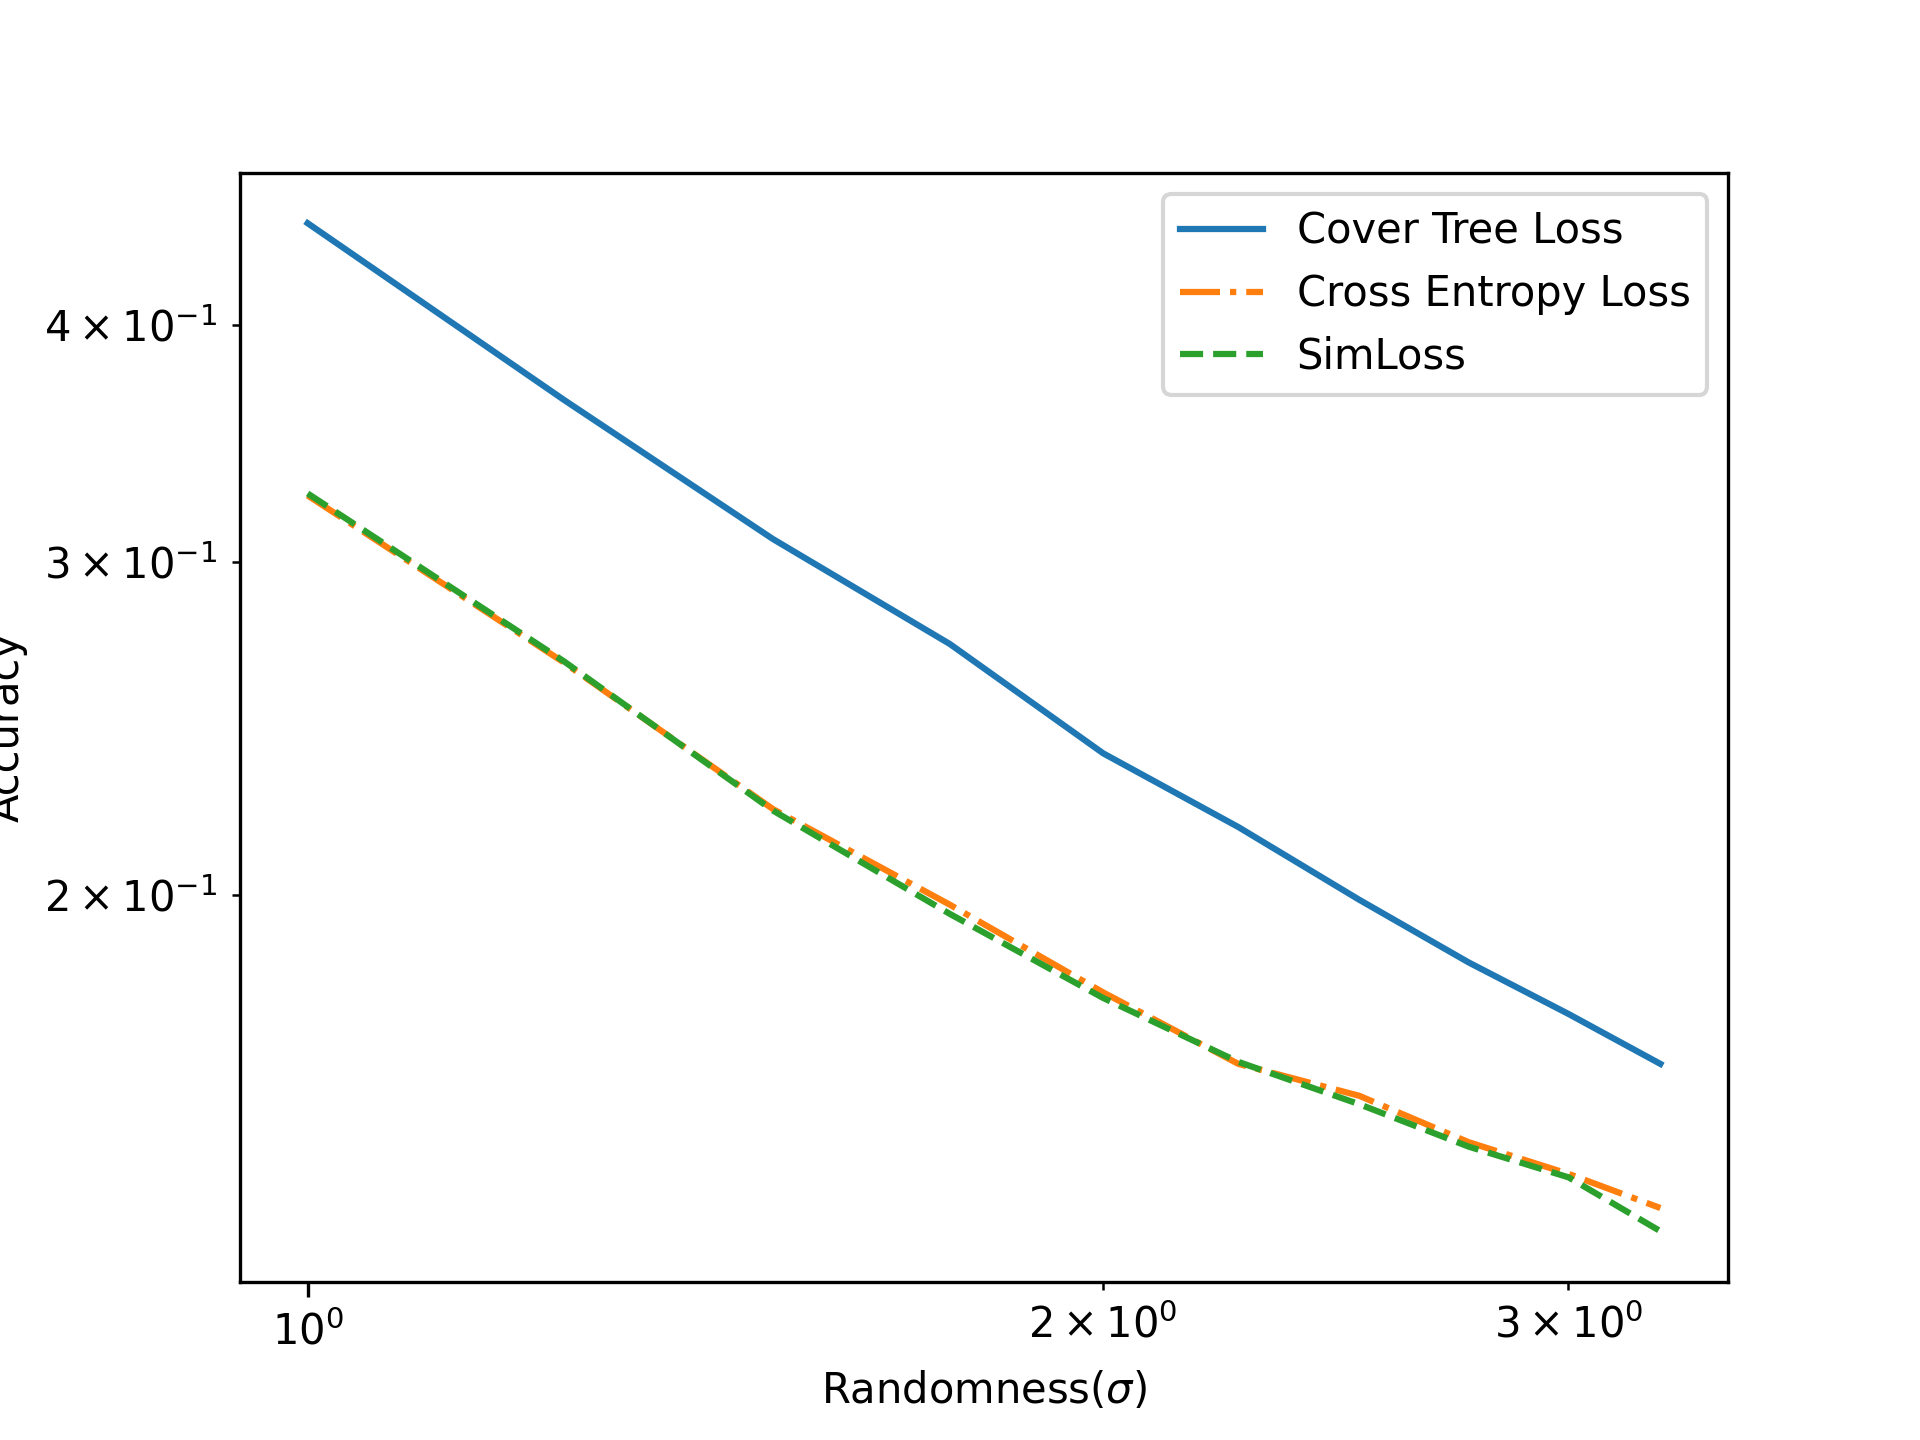
\includegraphics[width=0.8\columnwidth]{fig/images/accuracy_vs_sigma.png}
\end{center}
\end{frame}

%%%%%%%%%%%%%%%%%%%%

\begin{frame}{Experiments: Synthetic: Lemma Verification}
\begin{center}
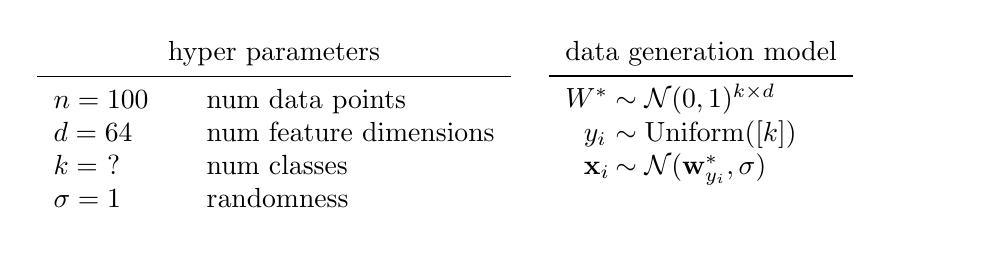
\begin{tikzpicture}
    \node[minimum height=1in]{\parbox{2in}{
        \begin{tabular}{p{0.6in}l}
            \multicolumn{2}{c}{hyper parameters} \\
            \midrule
            $n=100$ & num data points \\
            $d=64$ & num feature dimensions \\
            $k=~?$ & num classes \\
            $\sigma=1$ & randomness \\
        \end{tabular}
    }};
    \node[minimum height=1in] at (6.5,0) {\parbox{2in}{
        \begin{tabular}{ll}
            \multicolumn{2}{c}{data generation model} \\
            \midrule
            $W^*$ & \!\!\!\!\!\!$\sim \mathcal N(0,1)^{k\times d}$ \\
            ~~$y_i$ & \!\!\!\!\!\!$\sim \text{Uniform}([k])$ \\
            ~~$\x_i$ & \!\!\!\!\!\!$\sim \mathcal N(\w^*_{y_i}, \sigma)$ \\
            \\
        \end{tabular}
    }};
\end{tikzpicture}
%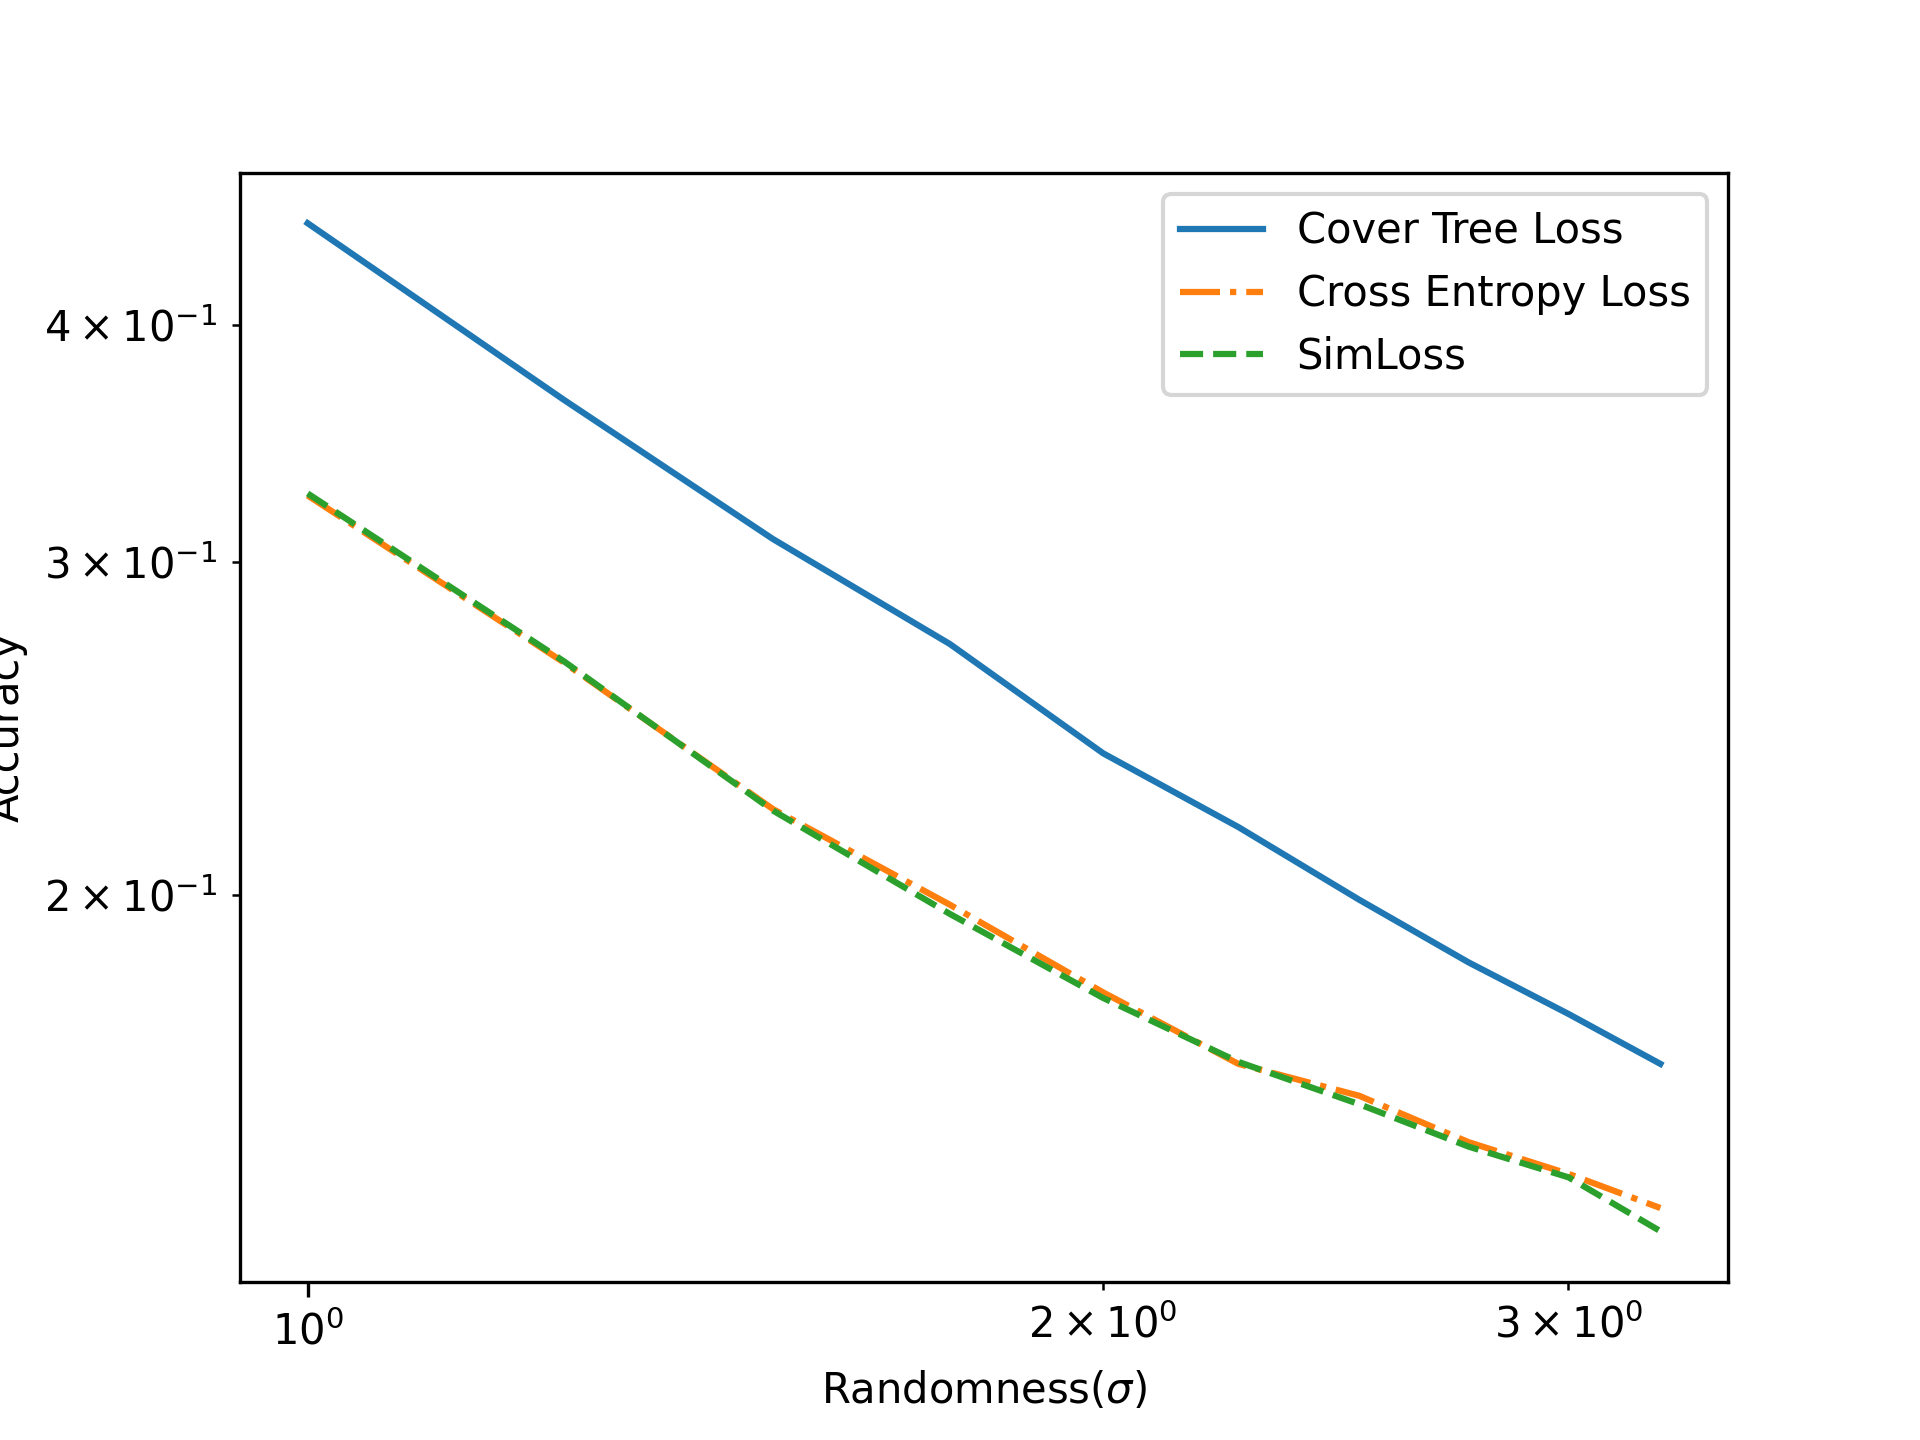
\includegraphics[width=0.8\columnwidth]{fig/images/accuracy_vs_sigma.png}
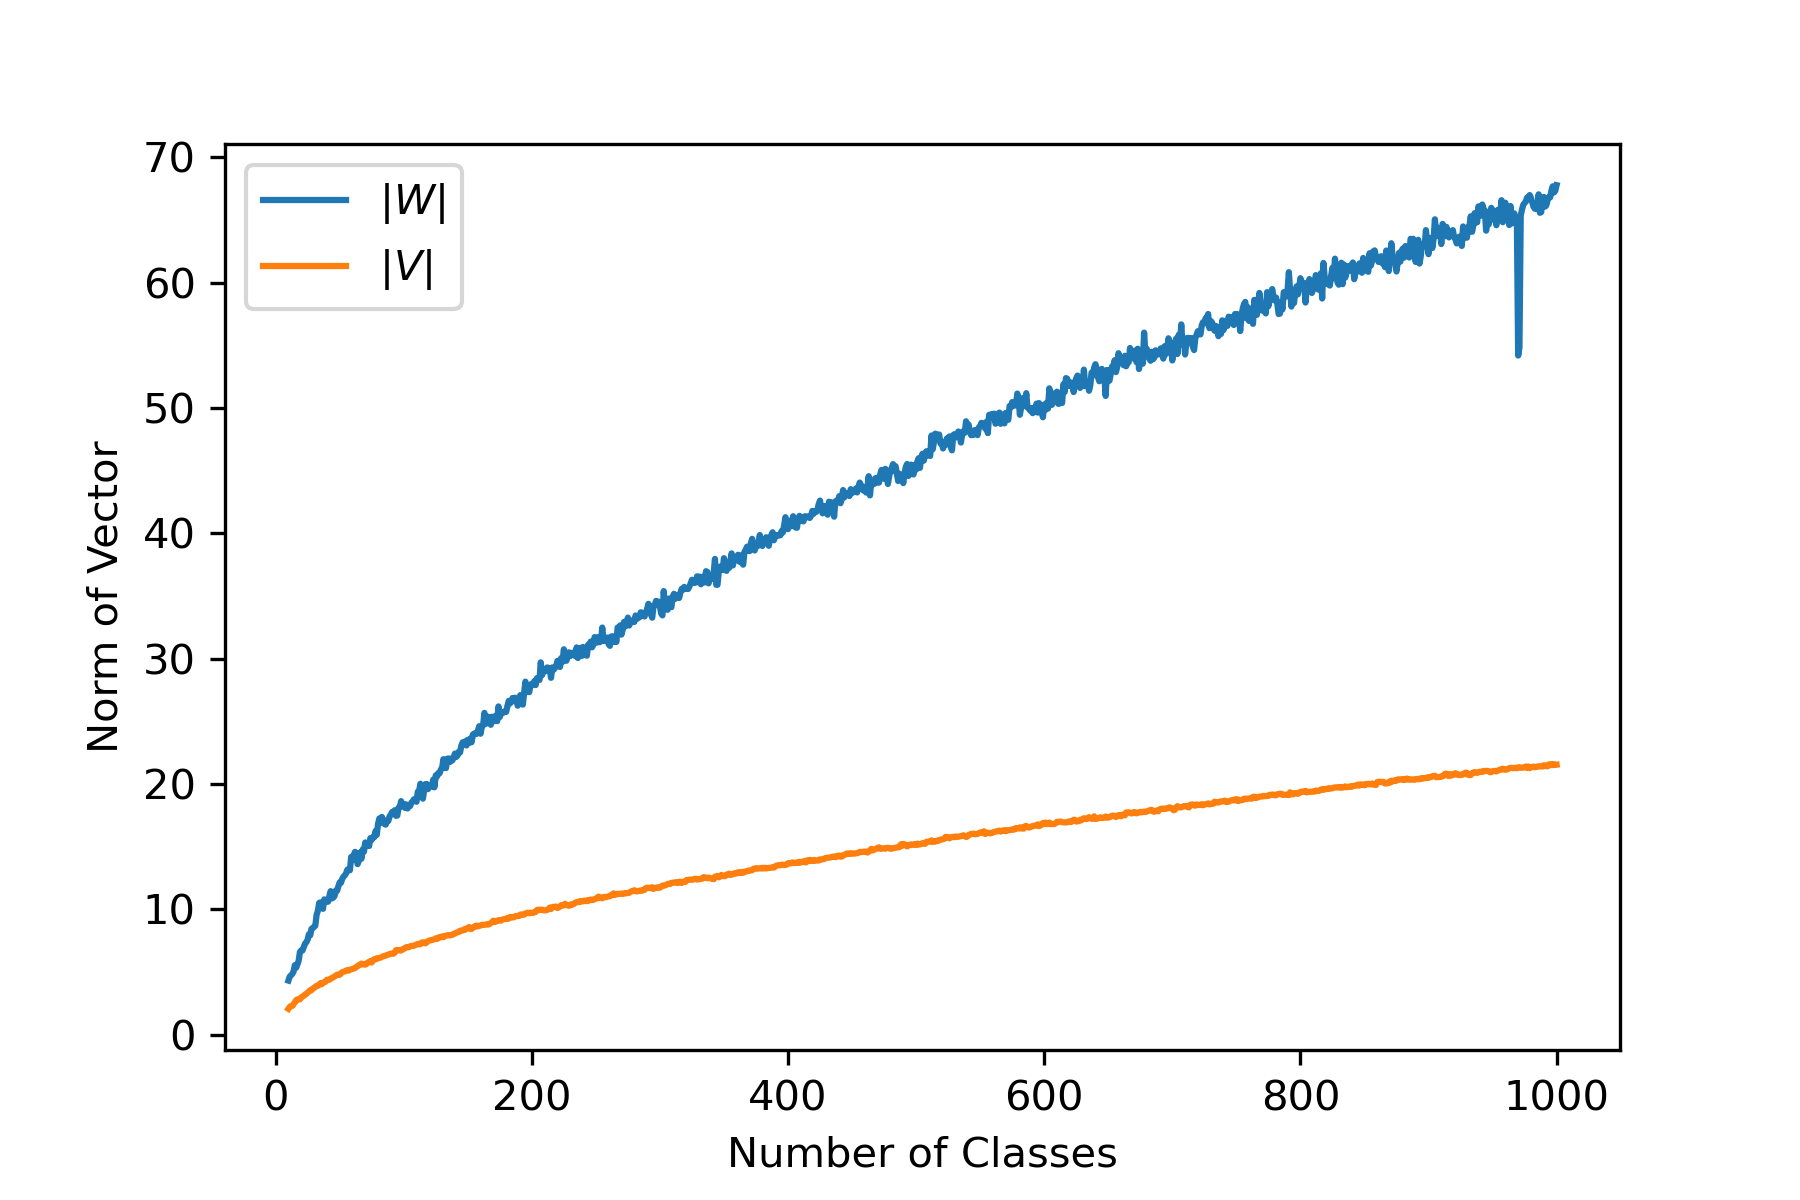
\includegraphics[width=0.8\columnwidth]{fig/images/class_v_norm.png}
\end{center}
\end{frame}


%%%%%%%%%%%%%%%%%%%%%%%%%%%%%%%%%%%%%%%%%%%%%%%%%%%%%%%%%%%%%%%%%%%%%%%%%%%%%%%%

%\begin{frame}{Experiments: Synthetic: Cover Tree}
%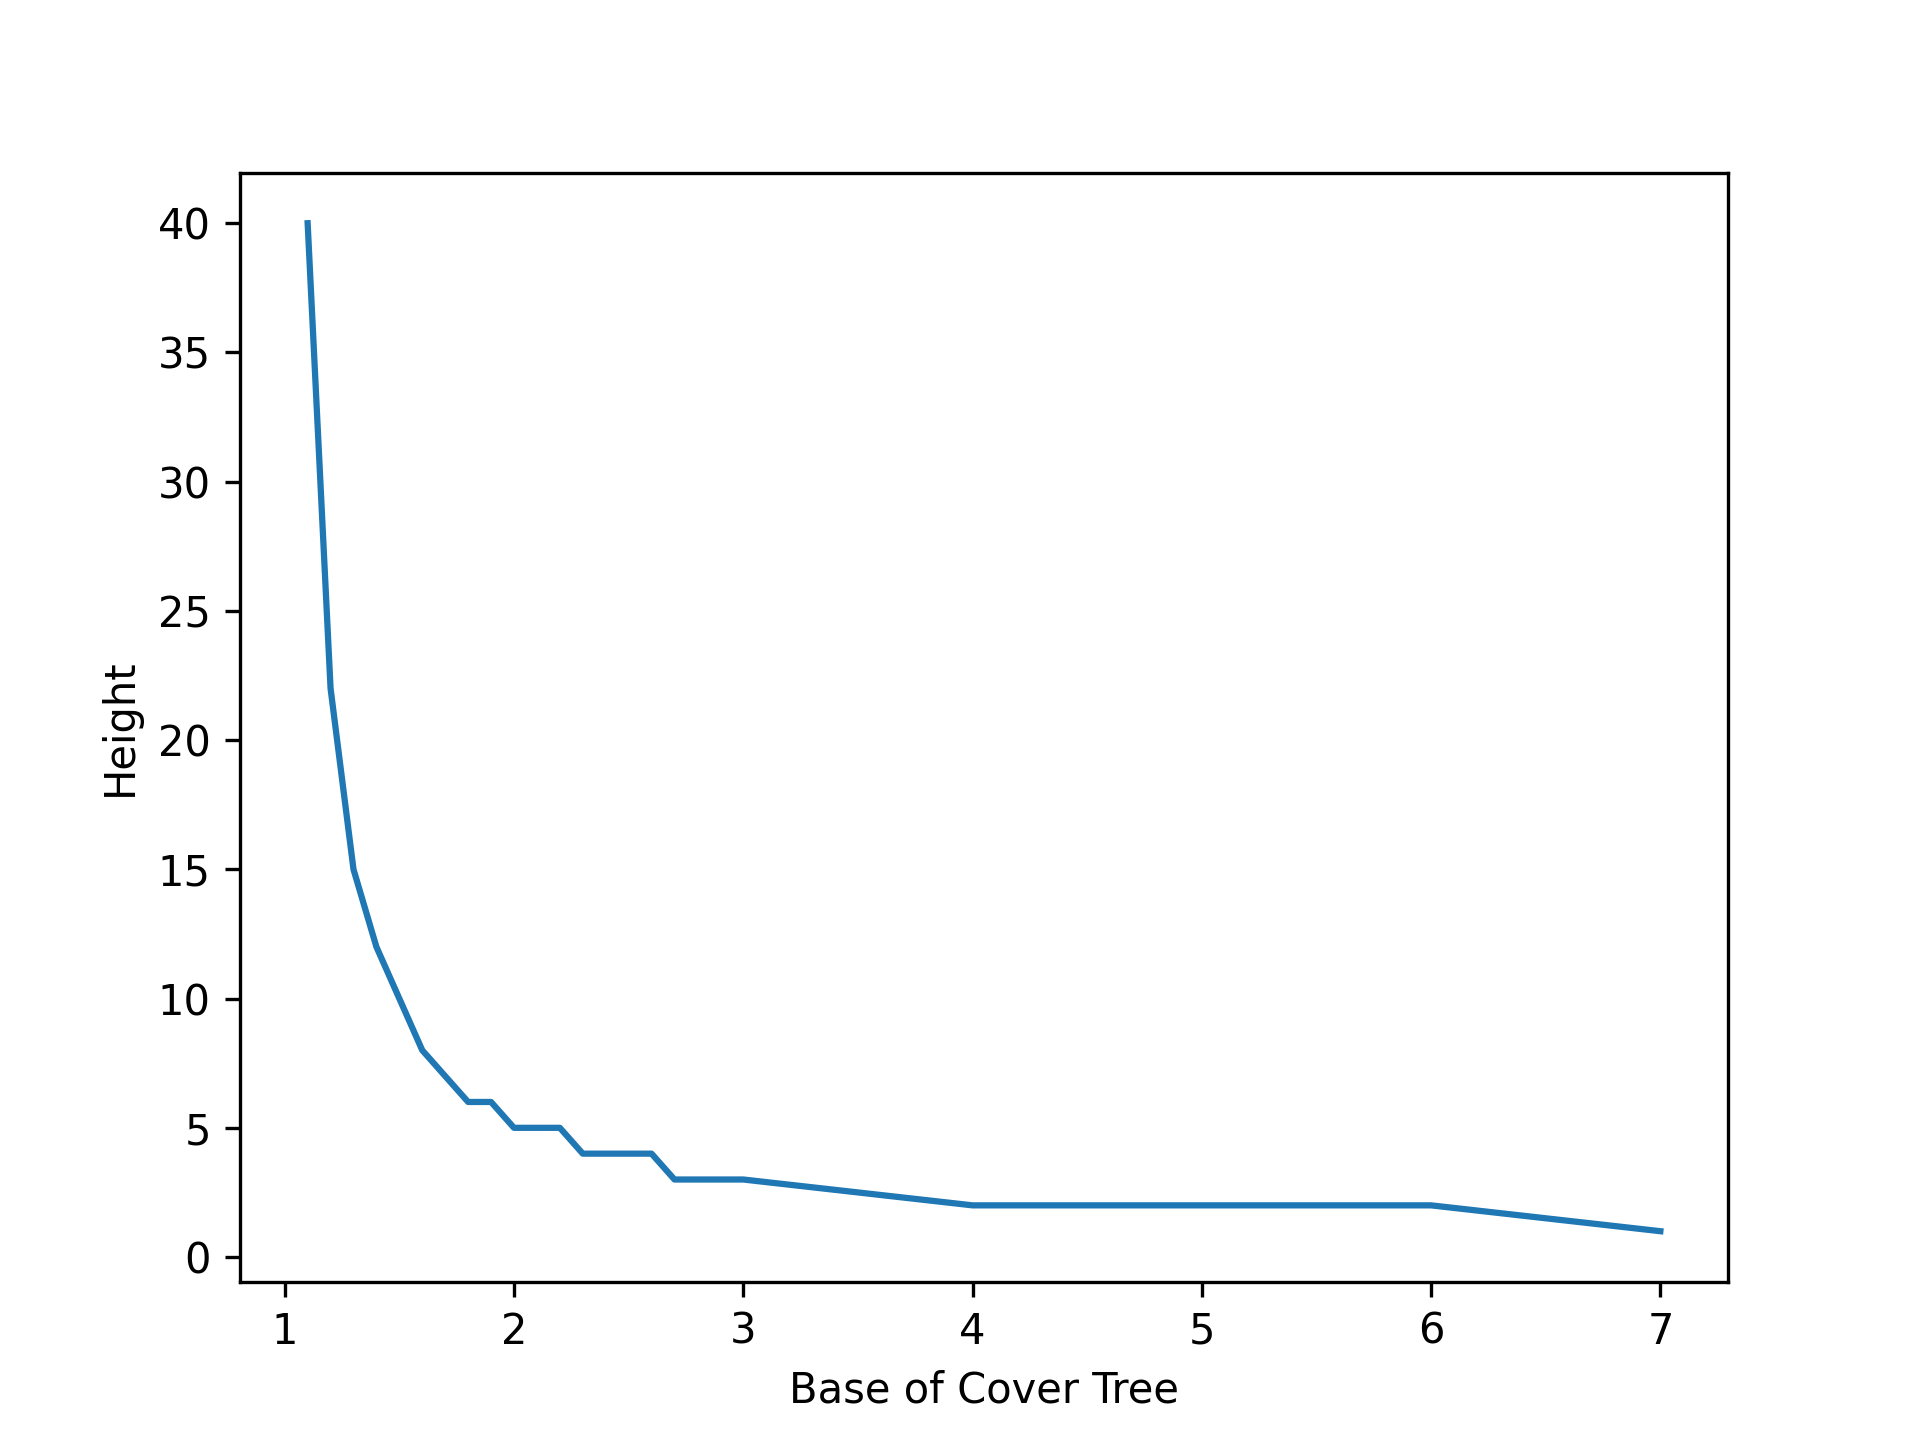
\includegraphics[width=\columnwidth]{fig/new_img/height_vs_base.png}
%\end{frame}

%%%%%%%%%%%%%%%%%%%%%%%%%%%%%%%%%%%%%%%%%%%%%%%%%%%%%%%%%%%%%%%%%%%%%%%%%%%%%%%%

%\begin{frame}{Experiments: Synthetic: Hyperparameters}
%\includegraphics[width=\columnwidth]{fig/new_img/accuracy_vs_base.png}
%\end{frame}

%%%%%%%%%%%%%%%%%%%%%%%%%%%%%%%%%%%%%%%%%%%%%%%%%%%%%%%%%%%%%%%%%%%%%%%%%%%%%%%%

\begin{frame}{Experiments: Synthetic: Bad Tree Structures}

Data generated as before.
Metric generated as:
\begin{align*}
    W^{\text{bad}}  &\sim \mathcal N(0,1)^{k\times d} \\
    d_\epsilon(i,j) &= \ltwo{(1-\epsilon)(\w_i^*-\w_j^*) + \epsilon(\w^{\text{bad}}_i - \w^{\text{bad}}_j)}
%\vspace{-0.1in}
\end{align*}
$\epsilon=0$ $\Rightarrow$ perfectly good metric

$\epsilon=1$ $\Rightarrow$ perfectly bad metric

    \vspace{-0.1in}
\begin{center}
\includegraphics[width=0.8\columnwidth]{fig/new_img/loss_vs_structure.png}
\end{center}
\end{frame}

\begin{frame}{Experiments: Real World}

\resizebox{\columnwidth}{!}{
\begin{tabular}{@{}lR{0.75in}R{0.75in}R{0.75in}R{0.75in}R{0.75in}R{0.75in}@{}}
%\toprule
                      & \multicolumn{2}{c}{CIFAR100}                           & \multicolumn{2}{c}{ImageNet}          & \multicolumn{2}{c}{Twitter} \\
%\cmidrule(r){1-1}
\cmidrule(l){2-3} 
\cmidrule(l){4-5} 
\cmidrule(l){6-7} 
                      & Top1 Acc        & SA                & Top1 Acc          & SA         & Top1 Acc          & SA \\
\midrule
tree loss             & \textbf{52.78}  & \textbf{65.90}    & \textbf{76.52}    & \textbf{88.22}    & \textbf{20.96}    & \textbf{50.54} \\
cross entropy loss    & 51.87           & 65.58             & 75.30             & 87.51             & 19.95             & 48.33 \\
simloss               & 52.43           & 65.82             & 76.24             & 87.98             & 19.96             & 48.32 \\
\bottomrule
\end{tabular}

}

    \vspace{0.2in}
Experimental Details:

\begin{itemize}
    \item CIFAR100/ImageNet: Image data, 100/1000 classes, ResNet features
        
        \citep{He2016DeepRL}

    \item Twitter: Text data, 80 classes, BERT features
        
        \citep{stoikos2020multilingual}

        \begin{itemize}
            \item predict the emoji (detailed sentiment) of a tweet about coronavirus
        \end{itemize}
\end{itemize}

\end{frame}



\begin{frame}{Summary (the end!)}

\begin{itemize}
\item more classes $\Rightarrow$ harder problem
\begin{itemize}
\item $k$: num classes, $d$: num dimensions, $n$: num data points
\end{itemize}
\begin{equation*}
\text{(cross entropy) generalization error}
=
O\left(\sqrt{\frac{kd}{n}}\right)
~~~~~~~~~~
\end{equation*}
\item real world classes are highly structured

\begin{itemize}
\item the doubling dimension $c <\!\!< k$

\end{itemize}
\begin{equation*}
\text{(conjectured optimal) generalization error}
=
O\left(\sqrt{\frac{cd}{n}}\right)
~~~~~~~~~~~~~~~~~~~~~~~~~~~~~~.
\end{equation*}

\item \textbf{contribution:} $U$/$V$-tree loss exploits arbitrary metric structure

\begin{equation*}
\text{(tree loss) generalization error} = 
\begin{cases}
\sqrt{\frac{d\log k}{n}} & c\le 1 \\
\sqrt{\frac{dk^{1-1/c}}{n}} & c>1 \\
\end{cases}
\end{equation*}

\item \textbf{bonus:} best performance on synthetic and real world experiments

\end{itemize}

\vspace{-4in}
\begin{tikzpicture}
    \node at (0,0) {};
    \node at (0,4in) {};

    %\node[anchor=north west,fill=white,minimum width=4.5in,minimum height=0.7in] at (0,2.94in) {};
    %\node[anchor=north west,fill=white,minimum width=4.5in,minimum height=0.74in] at (0,2.04in) {};
    %\node[anchor=north west,fill=white,minimum width=4.5in,minimum height=0.7in] at (0,1.04in) {};
    %\node[anchor=north west,fill=white,minimum width=4.5in,minimum height=0.3in] at (0,0.3in) {};
\end{tikzpicture}
\end{frame}










%\begin{frame}{Summary}

Theory predicts the following generalization errors:
\begin{itemize}
\item cross entropy is $O(\sqrt{k/n})$
\item tree loss is $\begin{cases}O(\sqrt{\log k/n})&c<=1\\O(\sqrt{k^{1-1/c}/n})&c>1\end{cases}$% if $c<=1$ else $O(\sqrt{k^{1-1/c}/n})$
\end{itemize}

\vspace{0.1in}
We hypothesize the optimal is $O(\sqrt{c/n})$

\vspace{0.1in}
Experiments:
\begin{itemize}
\item tree loss outperforms cross entropy loss:
\begin{itemize}
\item in all regimes of ablation study
\item even for bad trees! (lemma proves this is always true)
\end{itemize}
\item good performance on real world problems
\begin{itemize}
\item still working on gettint SOTA on ImageNet...
\end{itemize}
\end{itemize}

\vspace{0.1in}
\textbf{Tree Loss is easy to implement! Code available!}

\url{https://github.com/cora1021/TreeLoss}
\end{frame}

%\begin{frame}{(Informal) Main Result}

Let
\begin{itemize}
%\item $d$ features
\item $k$ be the number of classes, and%\uncover<2>{\textcolor{red}{, doubling dimension $c$}}
\item $n$ be the number of data points.
\end{itemize}

%The generalization error of the standard cross entropy loss decays as
%\begin{equation}
    %O(\sqrt{dk/n}).
%\end{equation}

Then almost all classification problems have
\begin{equation}
    \text{generalization error} = \Theta(\sqrt{k/n})
\end{equation}
in the PAC framework.

\uncover<2>{
    \textcolor{red}{(\emph{new})}
    Let
    \begin{itemize}
        \item $c$ be the doubling dimensionality of the classes.
    \end{itemize}
    Then we probide a simple algorithm with
    \begin{equation}
        \text{generalization error} = 
        \begin{cases}
            O(\sqrt{\log k/n}) & c \le 1 \\
            O(\sqrt{k^{1-c}/n}) & c > 1 \\
        \end{cases}
    \end{equation}
    and we conjecture that $\Theta(\sqrt{c/n})$ is optimal.
        %We provide a simple algorithm with generalization error
    %\begin{equation}
        %O(\sqrt{d\log k}/n)
    %\end{equation}
    }

\end{frame}

%\begin{frame}{Key Ideas}

%That is,
%\begin{equation}
%\end{equation}

\begin{block}{Lemma 1 (informal)}
%Let $W^*$ denote the ``optimal parameter matrix'' with ``infinite data''.
Stochastic Gradient Descent satisfies
\begin{equation}
\text{generalization error} = O\left( \frac{\lF{W^*}}{\sqrt{n}} \right)
    %\E_{\x,y}\ell(W^*, (\x,y)) = O\left( \frac{\lF{W^*}}{\sqrt{n}} \right)
\end{equation}
\end{block}

\uncover<1>{
Immediate corrollary of standard properties of SGD \citep{shalev2014understanding}.
}

\uncover<2>{
\vspace{-0.2in}
Recall that 
\begin{itemize}
\item $\displaystyle \lF{W} = \sqrt{\sum_{i=1}^d\sum_{j=1}^kW_{ij}^2}$ is the Frobenius norm
\item $W : \R^{k\times d}$
\end{itemize}
so under ``reasonable'' assumptions
\begin{equation}
\lF{W^*} = O(\sqrt{kd})
\end{equation}
recovering the known optimal bound.
}

\vspace{-1.3in}
\uncover<3>{
    \textbf{Algorithm Overview}
    \begin{itemize}
    \item introduce a new matrix $U$
    \item rewrite $\ell$ in terms of $U$ instead of $W$
    \item Lemma 1 $\Rightarrow$ generalization error = $O(\lF{U^*}/\sqrt{n})$
    \item show $\lF{U^*} <\!\!< \lF{W^*}$
    \end{itemize}
}
\vspace{1in}
\end{frame}



%\begin{frame}

\begin{block}{Assumption 1}
For each feature vector $\x$ in the data set,
\begin{equation}
\ltwo{\x} \le \rho.
\end{equation}
\end{block}

Most data satisfies this assumption:
\begin{itemize}
\item an image with $d$ pixels has $\rho=\sqrt{d}$
\item a standard Gaussian over $d$ has $\rho=\tilde O(\sqrt d)$ with high probability
\end{itemize}

\end{frame}

%\begin{frame}{SGD: intuition}
\includegraphics[width=\textwidth]{img/sgd}

{\tiny
Image Source: \url{https://sweta-nit.medium.com/batch-mini-batch-and-stochastic-gradient-descent-e9bc4cacd461}
}
\end{frame}

%\begin{frame}{$V$-Tree}
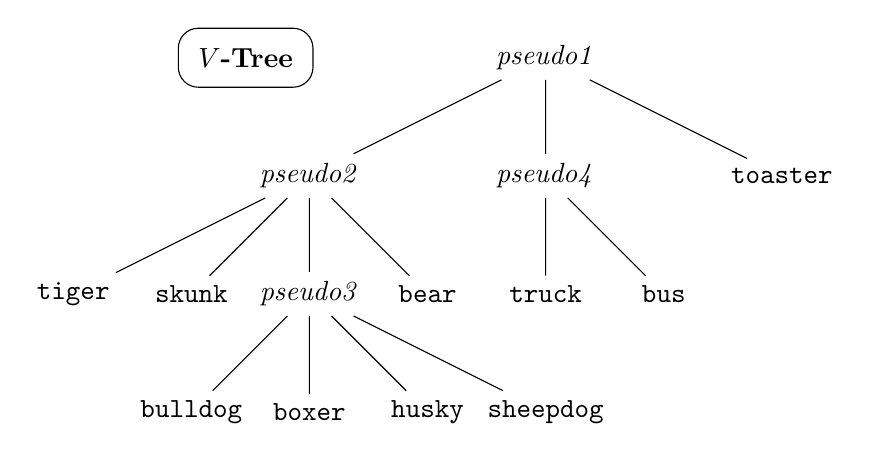
\begin{tikzpicture}
    [ level distance=1.5cm
    , level 1/.style={sibling distance=3cm}
    , level 2/.style={sibling distance=1.5cm}
    ]
\node[draw, rounded corners=0.1in, inner sep=0.1in] at (-1.5in,0){\textbf{$V$-Tree}};
\node {\textit{pseudo1}}
    child {node {\textit{pseudo2}}
      child {node {\texttt{tiger}}}
      child {node {\texttt{skunk}}}
      child {node {\textit{pseudo3}}
        child {edge from parent[draw=none]} % Added
        child {node {\texttt{bulldog}}}
        child {node {\texttt{boxer}}}
        child {node {\texttt{husky}}}
        child {node {\texttt{sheepdog}}}
      }
      child {node {\texttt{bear}}}
      child {edge from parent[draw=none]} % Added
      }
    child {node {\textit{pseudo4}}
      child {edge from parent[draw=none]} % Added
      child {node {\texttt{truck}}}
      child {node {\texttt{bus}}}
    }
    child {node {\texttt{toaster}}}
    ;

\end{tikzpicture}
\end{frame}



%%%%%%%%%%%%%%%%%%%%%%%%%%%%%%%%%%%%%%%%
\newcounter{finalframe}
\setcounter{finalframe}{\value{framenumber}}
%\input{slides/covertree/}

\begin{frame}[allowframebreaks]
\frametitle{Bibliography}
\bibliographystyle{ACM-Reference-Format}
%\bibliography{main}
\bibliography{paper,images}
\end{frame}

\setcounter{framenumber}{\value{finalframe}}

%%%%%%%%%%%%%%%%%%%%%%%%%%%%%%%%%%%%%%%%%%%%%%%%%%%%%%%%%%%%%%%%%%%%%%%%%%%%%%%%

\end{document}
